\documentclass[11pt,letterpaper]{article}
\usepackage[margin=1in]{geometry}
\usepackage{amsmath,amssymb}
\usepackage{graphicx}
\usepackage{booktabs}
\usepackage{xcolor}
\usepackage{framed}
\usepackage{listings}
\usepackage{enumitem}
\usepackage{hyperref}
\hypersetup{colorlinks=true, linkcolor=blue!60!black, urlcolor=blue!60!black}
\graphicspath{{figs/}}
\setlength{\parskip}{5pt}
\setlength{\parindent}{0pt}

\definecolor{boxbg}{RGB}{244,246,250}
\definecolor{exbg}{RGB}{255,244,230}
\definecolor{codebg}{RGB}{247,247,245}
\lstset{language=Python, basicstyle=\ttfamily\footnotesize, backgroundcolor=\color{codebg},
  frame=single, framerule=0pt, breaklines=true, columns=fullflexible, keepspaces=true,
  showstringspaces=false, commentstyle=\color{gray}, keywordstyle=\bfseries}

% boxes
\newenvironment{keybox}{\def\FrameCommand{\fboxsep=8pt\colorbox{boxbg}}\MakeFramed{\advance\hsize-\width\FrameRestore}}{\endMakeFramed}
\newenvironment{exercise}[1]{\def\FrameCommand{\fboxsep=8pt\colorbox{exbg}}\MakeFramed{\advance\hsize-\width\FrameRestore}\textbf{Implement it: #1}\par\smallskip}{\endMakeFramed}
\newcommand{\say}[1]{\begin{keybox}\textbf{How to say it.} #1\end{keybox}}

\newcommand{\LFS}{\mathrm{LFS}}
\newcommand{\SSl}{\mathrm{SS}_{\mathrm{lang}}}
\newcommand{\SSc}{\mathrm{SS}_{\mathrm{con}}}
\newcommand{\SSr}{\mathrm{SS}_{\mathrm{res}}}
\newcommand{\R}{\mathbb{R}}

\title{\textbf{From Zero to Defending LFS}\\[2mm]
\large Machine learning, language models, machine translation, and the statistics of measurement,\\
built around one instrument: the Language-Factor Share}
\author{Study guide for Waiz Khan}
\date{5 September 2026}

\begin{document}
\maketitle

\begin{keybox}
\textbf{What this is.} A self-contained course in everything you need to
explain and defend the LFS work to Professor Koehn, Professor Murray, other
faculty, and students, written for someone who has not yet learned the
fundamentals. It assumes you can program. Every chapter has ``Implement
it'' exercises in plain numpy, because the fastest way to own a formula is to
type it. Every LFS statement is tied to a number you can point to in the
repository.

\textbf{How to use it.} Read Chapter~\ref{ch:lfs} first, once, even if it is
hard; it tells you why everything else matters. Then work Chapters
\ref{ch:ml} to \ref{ch:stats} in order, doing the exercises. Return to
Chapter~\ref{ch:lfs} and it will be easy. Chapter~\ref{ch:defense} is the
question bank; practice it aloud. Chapter~\ref{ch:plan} is the schedule and
reading list.

\textbf{Compute rule.} The numpy exercises use synthetic data and run on your
Mac. Anything that loads a real language model runs on the CLSP cluster, as
always.
\end{keybox}

\begin{keybox}
\textbf{Do you need all of this to defend LFS?} No. Three tiers.

\textbf{Must know cold} (you will be asked, and a wrong answer costs
credibility): all of Chapter~\ref{ch:lfs}; from Chapter~\ref{ch:ml}, vectors,
norms and cosine, least squares and ridge, why held-out data; from
Chapter~\ref{ch:llm}, tokens and fertility, the residual stream and hidden
states per layer, mean pooling, what the logit lens assumes, fp16 versus
fp32; from Chapter~\ref{ch:stats}, two-way ANOVA and degrees of freedom,
Spearman, residualization and fixed effects, the cluster bootstrap and the
unit of generalization, preregistration; from Chapter~\ref{ch:mt}, parallel
corpora, translationese, MEXA's scoring rule, and the ``think in English''
papers.

\textbf{Should know} (this is what makes you credible to Koehn, Murray, and
faculty who work in these areas, and it lets you answer the follow-up
question, not just the first one): the rest of Chapters~\ref{ch:ml} to
\ref{ch:mt}.

\textbf{Later} (the long arc of a researcher, not this month): the measure
list in Chapter~\ref{ch:plan}, Block F.

The checklist in Chapter~\ref{ch:plan} marks the must-know items with a
star.
\end{keybox}

\tableofcontents
\clearpage

\section{Machine learning from zero}
\label{ch:ml}

\subsection{Why learn from data at all}

A program is a set of rules written by a person. For many tasks nobody can
write the rules. Nobody can list the rules that turn a German sentence into
an English one, or that say which word comes next in a paragraph, or that
tell a cat from a dog in pixels. What we do have, in enormous quantity, is
\emph{examples}: sentences with their translations, text with the word that
actually came next, pictures with labels.

Machine learning turns examples into a function by search. You fix a family
of functions with adjustable numbers (the \emph{parameters}), you write down a
score for how wrong a candidate function is on the examples (the
\emph{loss}), and you search for the parameter values that make the score
small (\emph{optimization}). ``Training'' is that search. It is the only
known way to get a translator that handles sentences no one anticipated,
because the rules come from the data, not from a person.

The price is the subject of this whole project. First, the function is only
as good as the data: a corpus that is mostly English produces a model that
is mostly English, whatever its size. Second, you cannot read the rules off
the parameters. A trained model is billions of numbers, and nobody can tell
by inspection what it learned about Persian. That is why measurement
instruments exist. LFS is one: it does not train anything, it measures what
training produced.

\subsection{The kinds of learning}

\begin{figure}[h]\centering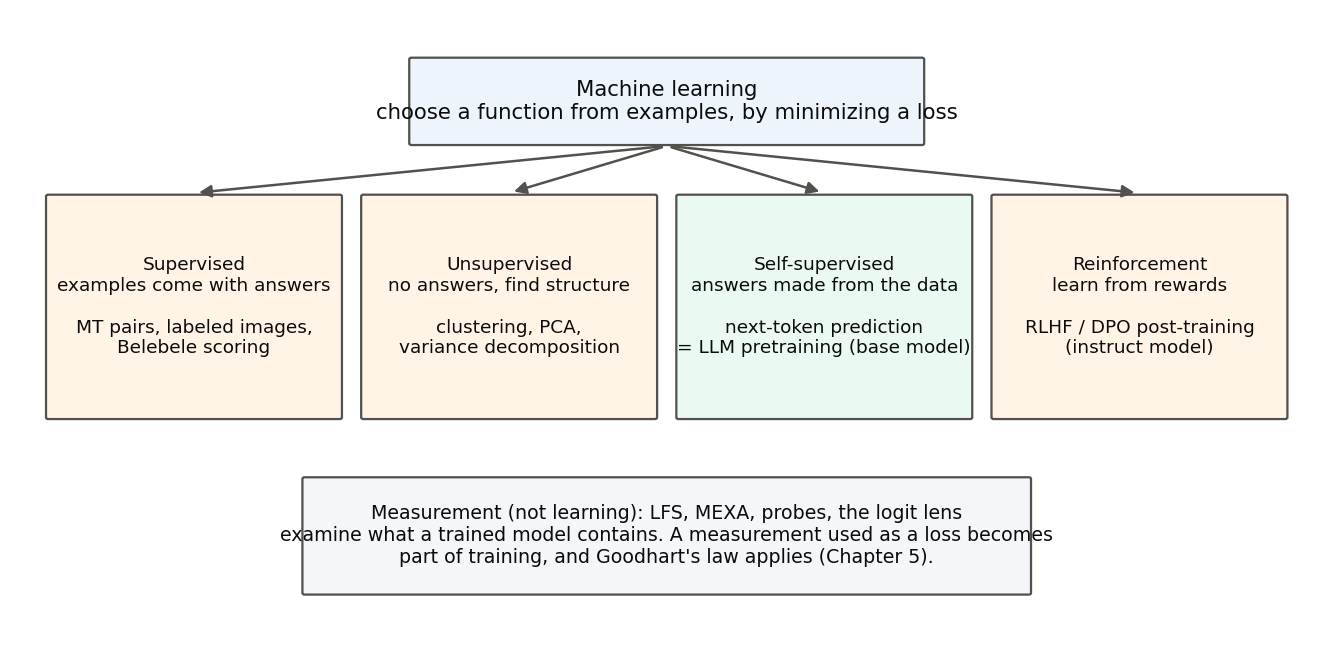
\includegraphics[width=0.95\linewidth]{fig_ml_types.png}
\caption{The kinds of learning, where an LLM's stages sit, and where LFS sits: outside learning, as measurement of what was learned.}\label{fig:types}\end{figure}

\begin{description}[leftmargin=3.2cm, style=nextline, itemsep=3pt]
\item[Supervised learning] Every example comes with the answer: a sentence
and its translation, a question and its correct option, an image and its
label. The model learns a map from input to answer, and the loss compares its
answer to the given one. Classical machine translation and the Belebele
scoring in this project are supervised in form.
\item[Unsupervised learning] No answers, only inputs. The goal is structure:
which examples cluster together, which directions carry the most variation
(PCA), how the data are distributed. The variance decomposition behind LFS
is unsupervised analysis of this kind, applied to a model's hidden states.
\item[Self-supervised learning] The trick that made LLMs possible: manufacture
the answer from the data itself. For text, hide the next word and ask the
model to predict it. Every position in every document becomes a labeled
example for free, so training can use trillions of tokens. LLM pretraining
is self-supervised; the resulting \emph{base model} is a next-token
predictor.
\item[Reinforcement learning] No fixed answers; the model acts, receives a
reward, and adjusts to get more reward. Used in post-training (RLHF, DPO)
to turn a base model into an assistant. The proposal's Aim 2 mentions
preference training of this kind for multilinguality.
\item[Measurement] Not learning. LFS, MEXA, probes, and the logit lens
examine what a trained model contains. The moment a measurement becomes a
training signal it becomes part of the loss, and Goodhart's law applies;
Chapter~\ref{ch:lfs} shows what happened when LFS was tried as one.
\end{description}

Everything below fits one sentence: you decide the \emph{shape} of the
function (a line, a network), the data decides its \emph{parameters}, and a
\emph{loss} says how badly any candidate does. A 70-billion-parameter
language model fits that sentence too.

\subsection{Vectors, matrices, and why a hidden state is a vector}

A vector $\mathbf{x} \in \R^D$ is a list of $D$ numbers. Two operations carry
this whole project.

\textbf{Dot product.} $\mathbf{x}\cdot\mathbf{y} = \sum_d x_d y_d$. It is
large when the vectors point the same way.

\textbf{Norm and cosine.} $\|\mathbf{x}\| = \sqrt{\mathbf{x}\cdot\mathbf{x}}$
is the length. Cosine similarity, $\cos(\mathbf{x},\mathbf{y}) =
\mathbf{x}\cdot\mathbf{y} / (\|\mathbf{x}\|\|\mathbf{y}\|)$, is the dot
product after removing length; it lies in $[-1, 1]$ and is what retrieval
metrics such as MEXA compare.

A matrix $W \in \R^{m\times n}$ turns a vector in $\R^n$ into one in $\R^m$:
$W\mathbf{x}$ is $m$ dot products, one per row. A neural network is a chain
of such multiplications with simple nonlinear functions in between. A
\emph{hidden state} is just the vector that sits between two of those
multiplications; in a language model it has $D$ coordinates (1024 for
Qwen3-0.6B, 4096 for Llama-3.1-8B) and there is one per token per layer.

\begin{exercise}{cosine similarity and a first look at anisotropy}
\begin{lstlisting}
import numpy as np
rng = np.random.default_rng(0)
def cos(a, b): return a @ b / (np.linalg.norm(a) * np.linalg.norm(b))
x, y = rng.normal(size=1024), rng.normal(size=1024)
print(cos(x, y))            # near 0: random high-dimensional vectors are nearly orthogonal
big = np.zeros(1024); big[7] = 40.0   # one huge shared coordinate ("massive activation")
print(cos(x + big, y + big))          # near 1: one coordinate makes everything look similar
\end{lstlisting}
The second print is the whole reason LFS standardizes coordinates before
measuring anything (Chapter~\ref{ch:lfs}).
\end{exercise}

\subsection{Linear regression and least squares}

Predict $y$ from $x$ with a line, $\hat y = w x + b$. The residual for one
point is $y_i - \hat y_i$. The least-squares choice of $(w, b)$ minimizes
$\sum_i (y_i - \hat y_i)^2$, the sum of squared residuals. Figure~\ref{fig:linreg}
shows the fit and the residuals. $R^2$ is the fraction of the variance of
$y$ that the line explains: $1 - \sum_i (y_i-\hat y_i)^2 / \sum_i (y_i - \bar
y)^2$.

\begin{figure}[h]\centering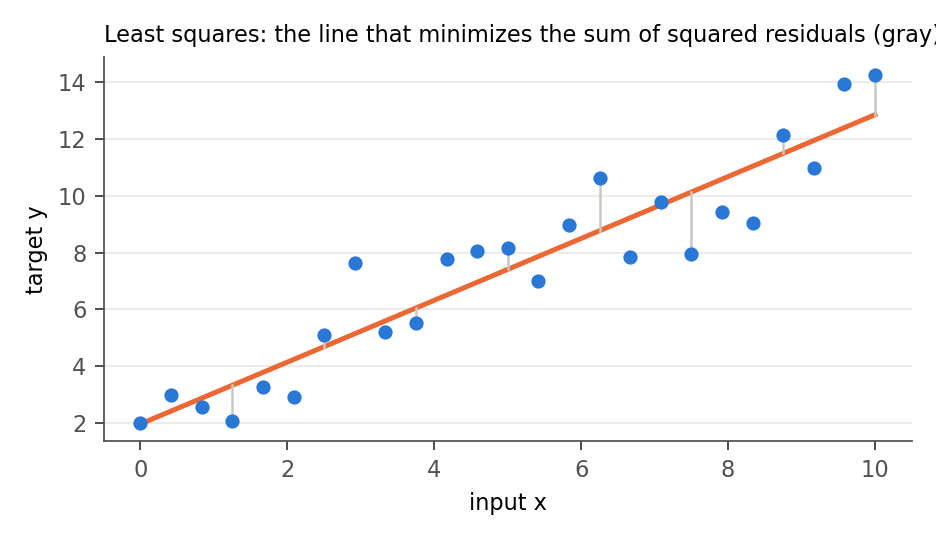
\includegraphics[width=0.7\linewidth]{fig_ml_linreg.png}
\caption{Least squares picks the line that makes the gray residuals as small as possible in the squared sense.}\label{fig:linreg}\end{figure}

With several inputs the same idea is $\hat{\mathbf{y}} = X\mathbf{w}$ and the
closed form is $\mathbf{w} = (X^\top X)^{-1} X^\top \mathbf{y}$. Adding a
penalty $\lambda\|\mathbf{w}\|^2$ gives \emph{ridge regression}, which keeps
weights small when inputs are many or correlated. The English-hub test in the
paper is ridge regression from one language's representations to another's.

\begin{exercise}{least squares two ways}
\begin{lstlisting}
x = np.linspace(0, 10, 50); y = 1.2 * x + 2 + rng.normal(0, 1.5, 50)
X = np.column_stack([x, np.ones_like(x)])
w_closed = np.linalg.lstsq(X, y, rcond=None)[0]
r2 = 1 - ((y - X @ w_closed)**2).sum() / ((y - y.mean())**2).sum()
print(w_closed, r2)
\end{lstlisting}
Keep this; the next exercise recovers the same $\mathbf{w}$ by gradient descent.
\end{exercise}

\subsection{Gradient descent}

For most models there is no closed form, so we descend. The gradient
$\nabla_\theta L$ is the vector of partial derivatives of the loss with
respect to each parameter; it points uphill. Gradient descent repeats
$\theta \leftarrow \theta - \eta\,\nabla_\theta L(\theta)$ with a small
\emph{learning rate} $\eta$ (Figure~\ref{fig:gd}). Too small and it crawls; too
large and it overshoots. Using a random \emph{batch} of examples per step
gives stochastic gradient descent; Adam adapts the step per parameter and is
what language models are trained with.

\begin{figure}[h]\centering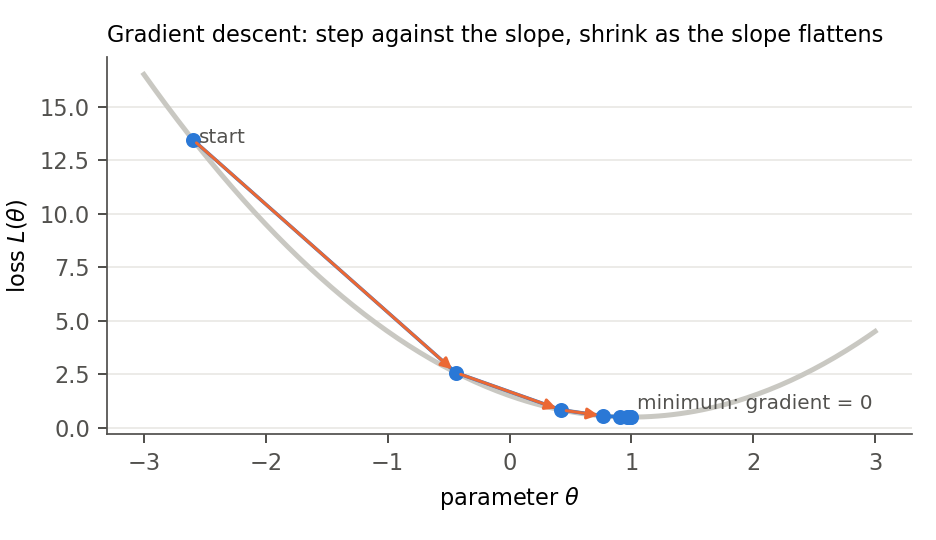
\includegraphics[width=0.66\linewidth]{fig_ml_gd.png}
\caption{Each step moves against the slope; steps shrink automatically as the slope flattens.}\label{fig:gd}\end{figure}

\begin{exercise}{gradient descent for the same line}
\begin{lstlisting}
w = np.zeros(2); eta = 0.01
for step in range(5000):
    pred = X @ w
    grad = 2 * X.T @ (pred - y) / len(y)     # derivative of mean squared error
    w -= eta * grad
print(w, w_closed)                           # should agree to a few decimals
\end{lstlisting}
Change \texttt{eta} to 0.1 and to 0.0001 and watch what happens.
\end{exercise}

\subsection{Classification: sigmoid, softmax, cross-entropy}

To predict a category, turn a score (a \emph{logit}) into a probability. For
two classes the sigmoid $\sigma(z) = 1/(1+e^{-z})$ does it; for $V$ classes
the softmax $p_v = e^{z_v} / \sum_u e^{z_u}$ does (Figure~\ref{fig:softmax}).
The loss is the negative log-probability of the true class, called
cross-entropy or negative log-likelihood (NLL): $-\log p_{\text{true}}$. It is
zero when the model is certain and right, and grows without bound as the
model assigns the truth less probability.

\begin{figure}[h]\centering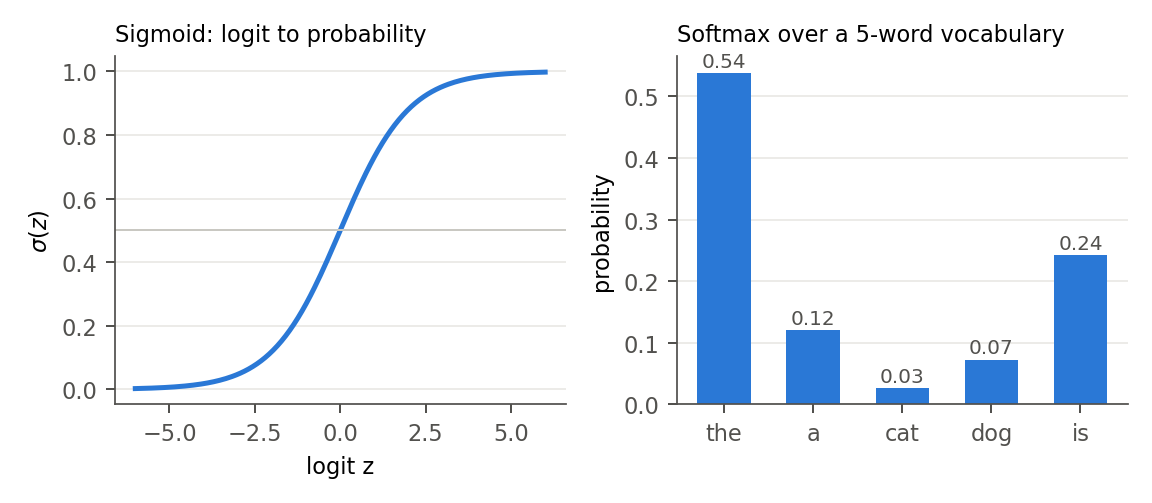
\includegraphics[width=0.85\linewidth]{fig_ml_logistic.png}
\caption{Left: sigmoid. Right: softmax over a tiny vocabulary. A language model does the right-hand thing over 150{,}000 tokens at every position.}\label{fig:softmax}\end{figure}

This is exactly the language-model objective: the classes are vocabulary
tokens, the input is the text so far, and the loss is the NLL of the next
token. Perplexity is $\exp(\text{mean NLL})$; a perplexity of 20 means the
model is, on average, as uncertain as a fair choice among 20 tokens.

\begin{exercise}{softmax, cross-entropy, and a gradient check}
\begin{lstlisting}
def softmax(z): z = z - z.max(); e = np.exp(z); return e / e.sum()
def nll(z, true): return -np.log(softmax(z)[true])
z = rng.normal(size=5); t = 2
# analytic gradient of NLL wrt logits is p - onehot(true)
g = softmax(z).copy(); g[t] -= 1
eps = 1e-5; num = np.array([(nll(z + eps*np.eye(5)[i], t) - nll(z - eps*np.eye(5)[i], t)) / (2*eps) for i in range(5)])
print(np.abs(g - num).max())     # ~1e-10: the analytic gradient is right
\end{lstlisting}
The subtraction of \texttt{z.max()} is numerical hygiene; it prevents overflow,
the same class of problem that made fp16 pooling fail on massive activations.
\end{exercise}

\subsection{Generalization: the only trustworthy score is on held-out data}

A model can fit its training data perfectly and be useless. Split data into
\emph{training} (fit), \emph{validation} (choose settings), and \emph{test}
(report once). Figure~\ref{fig:overfit} shows the classic picture: as
capacity grows, training error keeps falling while held-out error turns
around. Regularization (ridge penalties, early stopping, dropout) trades a
little training fit for better held-out behavior.

\begin{figure}[h]\centering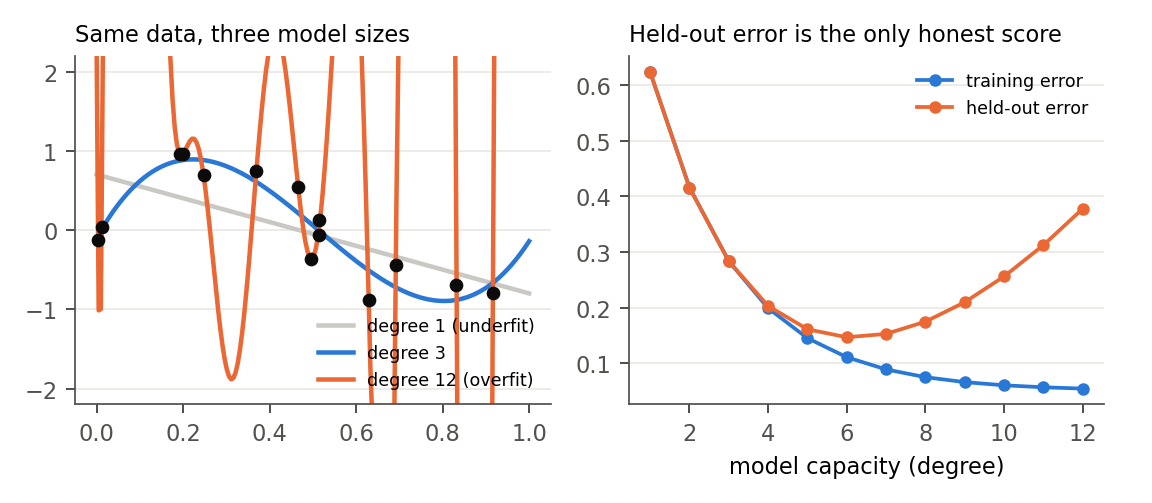
\includegraphics[width=0.9\linewidth]{fig_ml_overfit.png}
\caption{Left: three polynomials on the same points. Right: training versus held-out error as capacity grows.}\label{fig:overfit}\end{figure}

Two project habits are this principle applied to research itself. The
misalignment decomposition scores each map on \emph{held-out} sentences, and it
found that the flexible nonlinear map had been overfitting to same-document
leakage. And preregistration is early stopping for the analyst: decide the
test before you see the data.

\begin{exercise}{watch overfitting happen}
Fit polynomials of degree 1 to 12 to 15 noisy points from $\sin(2\pi x)$ with
\texttt{np.polyfit}; compute training error and error on 200 fresh points;
plot both against degree. Then repeat with 150 training points and note how
the turnaround moves.
\end{exercise}

\subsection{Neural networks in one picture}

A multilayer perceptron (MLP) is $\hat{\mathbf y} = W_2\,\phi(W_1 \mathbf x +
\mathbf b_1) + \mathbf b_2$ where $\phi$ is a nonlinearity applied
elementwise (ReLU $\max(0,z)$, or the smoother GELU). Without $\phi$ the two
matrices would collapse into one; the nonlinearity is what lets the network
represent anything (Figure~\ref{fig:mlp}). Training is gradient descent on
all the weights; \emph{backpropagation} is the chain rule applied
layer by layer to get the gradient efficiently, and libraries do it for you
(autograd).

\begin{figure}[h]\centering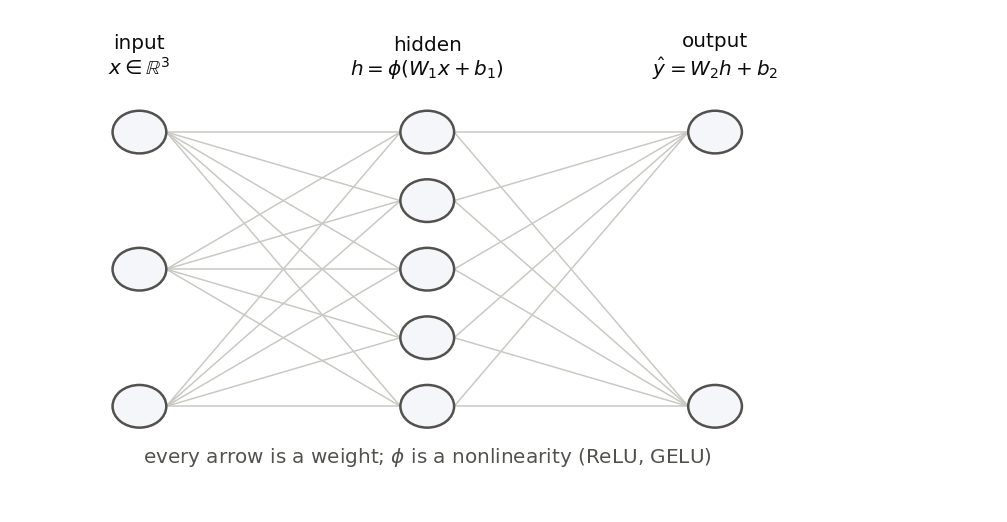
\includegraphics[width=0.72\linewidth]{fig_ml_mlp.png}
\caption{An MLP: two matrix multiplications with a nonlinearity between them. Each transformer block contains one of these, applied to every token position independently.}\label{fig:mlp}\end{figure}

\begin{exercise}{a two-layer network on XOR, gradients by hand}
\begin{lstlisting}
X = np.array([[0,0],[0,1],[1,0],[1,1]], float); y = np.array([0,1,1,0], float)
W1 = rng.normal(0, 1, (2, 8)); b1 = np.zeros(8); W2 = rng.normal(0, 1, 8); b2 = 0.0
for step in range(5000):
    h_pre = X @ W1 + b1; h = np.maximum(0, h_pre)          # ReLU
    z = h @ W2 + b2; p = 1 / (1 + np.exp(-z))               # sigmoid output
    loss = -np.mean(y*np.log(p+1e-9) + (1-y)*np.log(1-p+1e-9))
    dz = (p - y) / 4                                        # dLoss/dz
    dW2 = h.T @ dz; db2 = dz.sum()
    dh = np.outer(dz, W2) * (h_pre > 0)                     # chain rule through ReLU
    dW1 = X.T @ dh; db1 = dh.sum(0)
    for P, g in ((W1, dW1), (W2, dW2)): P -= 0.5 * g
    b1 -= 0.5 * db1; b2 -= 0.5 * db2
print(np.round(p, 2))       # approaches [0, 1, 1, 0]
\end{lstlisting}
Remove the ReLU (\texttt{h = h\_pre}) and confirm the network can no longer
solve XOR: a linear model cannot.
\end{exercise}

\subsection{Embeddings, PCA, and effective rank}

An \emph{embedding} turns a discrete thing (a word, a token, a language) into
a vector so that geometry can carry meaning: similar things get nearby
vectors. Token embeddings are the first layer of a language model.

To look at a cloud of vectors, use principal component analysis (PCA): center
the data, compute the covariance, take its eigenvectors. The top eigenvectors
are the directions of largest variance; the eigenvalues say how much variance
each carries. The singular value decomposition (SVD) computes the same thing
directly from the data matrix. From the spectrum you get the \emph{effective
rank}: how many directions really carry variance (entropy of the normalized
spectrum, exponentiated, or the participation ratio $(\sum\lambda)^2/\sum\lambda^2$).
The paper uses these to show that a collapsed model lost dimensions even when
its LFS ratio looked fine.

\begin{exercise}{PCA and effective rank of a synthetic representation cloud}
\begin{lstlisting}
Z = rng.normal(size=(500, 64)) @ np.diag(np.r_[np.linspace(5, 1, 8), 0.1*np.ones(56)])
Zc = Z - Z.mean(0)
lam = np.linalg.eigvalsh(Zc.T @ Zc / len(Zc))[::-1]
w = lam / lam.sum()
print("participation ratio:", lam.sum()**2 / (lam**2).sum())
print("entropy rank:", np.exp(-(w[w>0] * np.log(w[w>0])).sum()))
\end{lstlisting}
Both should say ``about 8'': the cloud lives in 8 real directions plus noise.
\end{exercise}

\subsection{Vocabulary you will hear in every meeting}

\begin{description}[leftmargin=2.2cm, style=nextline, itemsep=1pt]
\item[parameters / weights] the numbers the data chooses; \emph{hyperparameters} are the ones you choose (learning rate, size).
\item[epoch, batch, step] one pass over the data; a slice of it; one gradient update.
\item[pretraining] training a base model on raw text with the next-token loss; a \emph{checkpoint} is a saved set of weights.
\item[fine-tuning] continuing training on a smaller, targeted dataset; \emph{instruction tuning} is fine-tuning on prompt--response pairs.
\item[inference] running the trained model; \emph{forward pass} is one evaluation of the network.
\item[seed] the random-number starting point; three seeds means three independent training runs.
\item[in-distribution / held-out] data like the training data / data deliberately kept away from every choice you made.
\end{description}

\clearpage
\section{How a large language model works}
\label{ch:llm}

A large language model (LLM) is a function that takes a sequence of tokens
and returns a probability distribution over the next token. Everything
else, chat, translation, reasoning, is that function applied repeatedly.
Figure~\ref{fig:pipeline} is the whole pipeline; the rest of the chapter
walks through each box, and says at each step what LFS reads.

\begin{figure}[h]\centering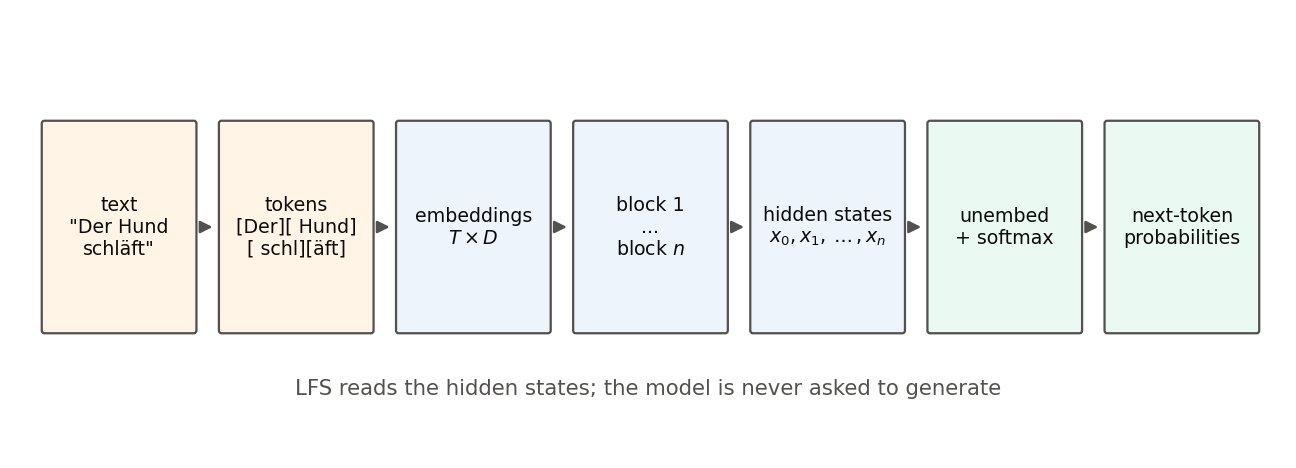
\includegraphics[width=\linewidth]{fig_llm_pipeline.png}
\caption{Text in, next-token probabilities out. LFS is computed from the hidden states in the middle and never asks the model to generate.}\label{fig:pipeline}\end{figure}

\subsection{Tokenization and fertility}

Text is split into \emph{tokens}: pieces of words drawn from a fixed
vocabulary of 30{,}000 to 250{,}000 entries, learned by byte-pair encoding
(BPE) or a similar scheme so that frequent strings become single tokens.
``The'' is one token; ``schläft'' may be two; an Arabic or Persian word may be
five or six because the vocabulary saw little of those scripts.

\emph{Fertility} is the number of tokens per word (or per character),
usually reported relative to English. High fertility means a language pays
more tokens for the same meaning, gets less content into a fixed context
window, and costs more per sentence. Fertility matters for LFS in two ways.
Mean pooling averages a different number of tokens per language, and the
tokenizer itself carries language identity into the embedding layer. That is
why fertility is a control variable in every validity analysis, and why the
paper reports that per-language contributions to the language variance
correlate with fertility at $+0.42$ to $+0.64$.

\subsection{Embeddings and the residual stream}

Each token id selects a row of the embedding matrix $E \in \R^{V\times D}$.
The resulting $D$-dimensional vector is the starting value of the
\emph{residual stream} for that position. Modern models add position
information through rotary embeddings inside attention rather than by adding
a position vector, but the picture is the same: position $t$ has a vector
$\mathbf x^{(0)}_t \in \R^D$.

The residual stream is a running sum. Each of the $n$ blocks reads the
stream, computes an update, and adds it back:
\[
\mathbf x^{(k)} = \mathbf x^{(k-1)} + \mathrm{Attn}_k\!\big(\mathrm{norm}(\mathbf x^{(k-1)})\big) + \mathrm{MLP}_k\!\big(\mathrm{norm}(\cdot)\big).
\]
The \emph{hidden state at layer $k$} is $\mathbf x^{(k)}$. Hugging Face
returns $n+1$ hidden states per token: index 0 is the embedding output and
index $k$ is the stream after block $k$. In the project's results a 28-block
model therefore has 29 ``layers'', and layer 0 is the embedding layer. This
additive structure is why it is meaningful to compare states across layers at
all: they all live in the same $D$-dimensional space and each layer is an
increment.

\begin{figure}[h]\centering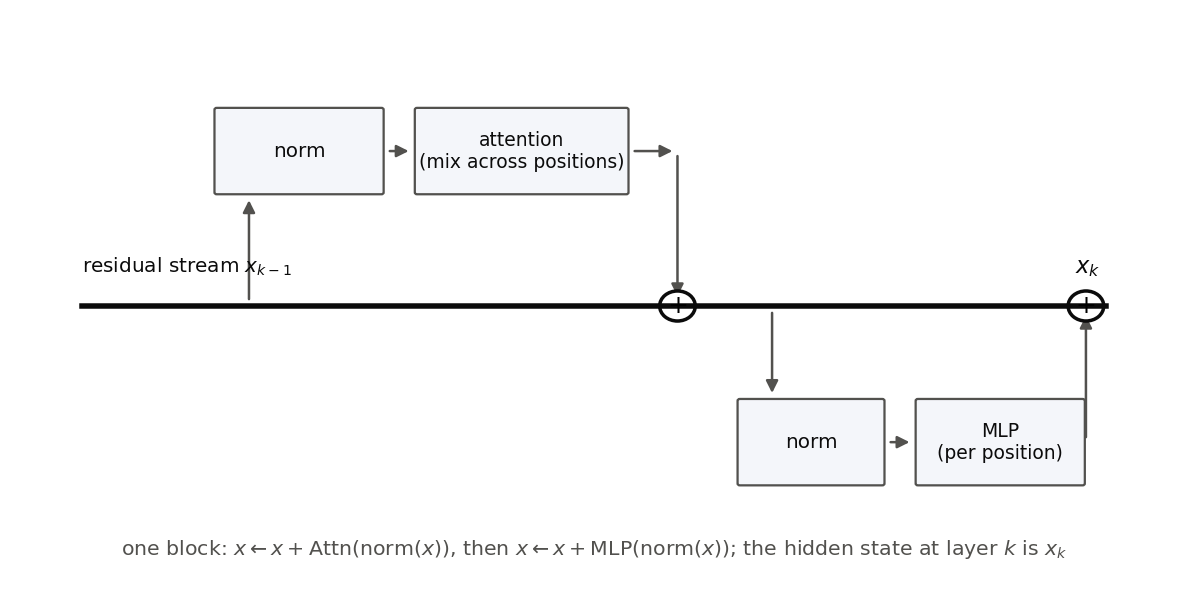
\includegraphics[width=0.9\linewidth]{fig_llm_block.png}
\caption{One transformer block. The horizontal line is the residual stream; the two branches add their outputs back into it.}\label{fig:block}\end{figure}

\subsection{Attention}

Attention is how a position pulls information from earlier positions. For
each position compute a query $\mathbf q$, a key $\mathbf k$, and a value
$\mathbf v$ (three matrix multiplications). The score between position $i$
and an earlier position $j$ is $\mathbf q_i\cdot\mathbf k_j/\sqrt{d}$; a
softmax over $j$ turns the scores into weights (Figure~\ref{fig:attn}); the
output is the weighted sum of the values $\sum_j w_{ij}\mathbf v_j$. A
\emph{causal mask} forbids looking at later positions, which is what makes
the model a left-to-right predictor. Multi-head attention runs this several
times in parallel with smaller $d$ and concatenates.

\begin{figure}[h]\centering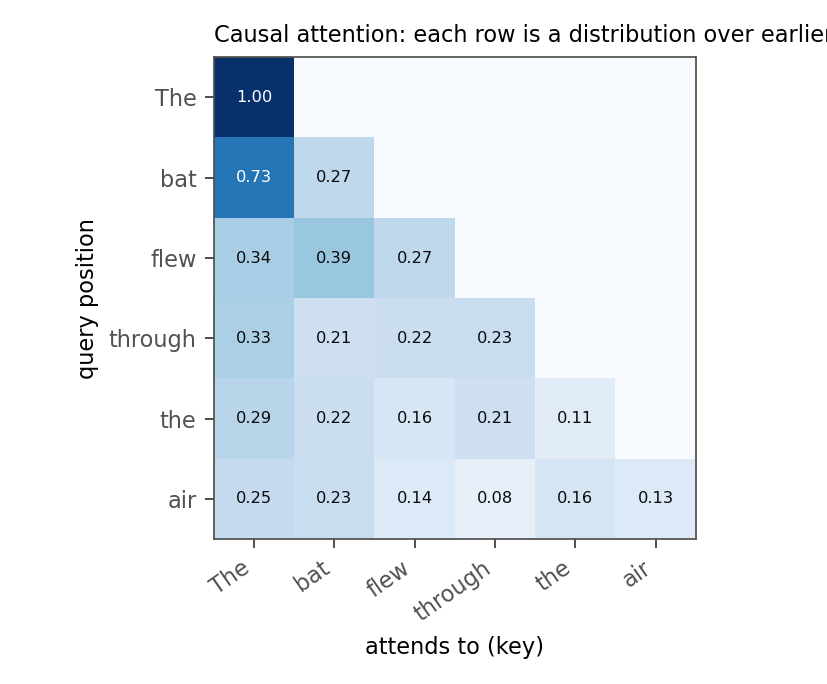
\includegraphics[width=0.62\linewidth]{fig_llm_attention.png}
\caption{Causal attention weights for one head: each row sums to one and only looks left.}\label{fig:attn}\end{figure}

The content-transfer experiment in the paper is attention in action: a
context sentence in Russian lowers the loss on an English target only if
attention at some layer moves information from the Russian tokens into the
English positions. The attention analysis measured exactly that mass, and
found it peaks just below the LFS minimum.

\begin{exercise}{single-head causal attention in numpy}
\begin{lstlisting}
T, D, d = 6, 32, 16
X = rng.normal(size=(T, D))                     # residual stream for 6 positions
Wq, Wk, Wv = (rng.normal(0, D**-0.5, (D, d)) for _ in range(3))
Q, K, V = X @ Wq, X @ Wk, X @ Wv
scores = Q @ K.T / np.sqrt(d)
scores[np.triu_indices(T, 1)] = -np.inf         # causal mask: no looking ahead
W = np.exp(scores - scores.max(1, keepdims=True)); W /= W.sum(1, keepdims=True)
out = W @ V                                     # (T, d): what each position gathered
print(np.round(W, 2))                           # lower-triangular, rows sum to 1
\end{lstlisting}
Now apply the same $W$ to \texttt{V} scaled by 100 and confirm \texttt{W} does
not change: attention weights depend on $Q$ and $K$, not on the scale of $V$.
\end{exercise}

\subsection{The MLP and normalization}

The MLP in each block is the two-matrix network of Chapter~\ref{ch:ml}, applied
to each position separately, with a hidden width of about $4D$ (SwiGLU
variants use a gated form). It is where much of a model's factual knowledge
appears to be stored, and it is the part that does not mix positions.

Normalization (LayerNorm or RMSNorm) rescales each position's vector to a
standard size before each branch. Modern models are \emph{pre-norm}: the
branch sees a normalized copy, but the residual stream itself is not
normalized, which is why a few coordinates of the stream can grow into
\emph{massive activations}, values hundreds of times larger than their
neighbors. Those coordinates dominate any unstandardized distance, overflow
fp16 sums, and are the reason LFS z-scores every coordinate jointly before
decomposing.

\subsection{From the last layer to a probability}

After the last block, a final norm and the \emph{unembedding} matrix $W_U \in
\R^{D\times V}$ turn the $D$-vector at each position into $V$ logits; softmax
gives the next-token distribution. Some models tie $W_U$ to the embedding
matrix. The \emph{logit lens} applies $W_U$ to an intermediate hidden state
and reads off the top token; it is a heuristic that presumes intermediate
states already live near the output space. The project measured that
presumption: mid-stack states reach a maximum cosine of about 0.10 to any
row of $W_U$ (0.20 at the final layer). Logit-lens readouts of middle layers,
including the ``LLMs think in English'' measure, rest on weak geometry.

\subsection{Training, base models, and post-training}

Training (Figure~\ref{fig:training}) is gradient descent on the next-token
cross-entropy over trillions of tokens, in batches, with Adam and a learning
rate that warms up and then decays. The model is always shown the true prefix
(\emph{teacher forcing}), so training is fully parallel across positions. The
output is a \emph{base} checkpoint: a next-token predictor, not a chatbot.
Post-training adds \emph{supervised fine-tuning} on instruction--response
pairs and often \emph{preference optimization} (RLHF, DPO) to produce an
\emph{instruct} model. Every model measured in the paper is a base checkpoint;
whether instruction tuning moves the LFS profile is an open, cheap
experiment.

\begin{figure}[h]\centering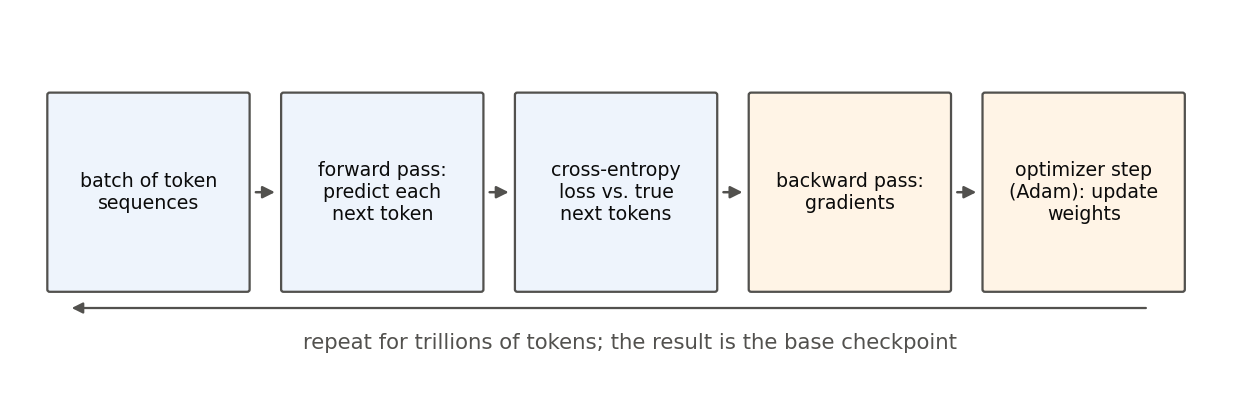
\includegraphics[width=\linewidth]{fig_llm_training.png}
\caption{The training loop. Nothing in it mentions languages; multilinguality is whatever the data induces.}\label{fig:training}\end{figure}

Two consequences for multilinguality. First, the data mix decides what is
learned: models trained mostly on English are English-centric by
construction, and the proposal's Aim 2 is about changing the data or the loss
to fix that. Second, ``scale'' (parameters and tokens) and ``recipe'' (mix,
tokenizer, curriculum) are confounded across labs, which is why the paper
calls the recipe-over-scale finding descriptive.

\subsection{Inference and scoring}

At inference the model produces a distribution at each step; you pick a
token (greedy, or sampling with a temperature) and repeat. For evaluation
you often do not generate at all: you feed a fixed continuation and read off
its probability. The teacher-forced NLL of a target sentence given a context
is exactly what the content-transfer test measures, and Belebele scoring
compares the log-likelihoods of the four answer options.

\subsection{Precision}

fp32 uses 32 bits per number; fp16 uses 16 with a small exponent range (max
about 65{,}000); bf16 uses 16 with fp32's exponent range but fewer digits.
Models are run in bf16 or fp16 for speed. Sums of squares of massive
activations overflow fp16, so pooling and every statistic in the project are
accumulated in fp32, and BLOOM, which was trained in bf16, is never run in
fp16. Two documented errors in the discrepancy ledger came from exactly
this; be ready to tell them.

\subsection{Interpretability handles you will use}

\begin{description}[leftmargin=2.6cm, style=nextline, itemsep=1pt]
\item[hidden states] the residual stream per layer, via \texttt{output\_hidden\_states=True}. The raw material of LFS.
\item[pooling] collapsing a sentence's token states into one vector: mean over tokens (used here), last token, or unit-normalized mean. Pooling is part of the measurement definition; absolute LFS values change with it, rankings much less.
\item[linear probe] a logistic regression trained on hidden states to predict a label (here: which language). High accuracy means the information is linearly present. Language stays decodable at 0.875 to 0.886 at every layer even where LFS is lowest.
\item[logit lens] unembed an intermediate state; see above for its limits.
\item[activation patching] copy a hidden state from one run into another and measure what changes; the causal tool Dumas et al.\ use to separate language from concept.
\item[CKA] a similarity index between two sets of representations, invariant to rotation and scale; used as a comparator in the fault test suite.
\end{description}

\begin{exercise}{hidden states for one sentence in three languages (run on CLSP)}
\begin{lstlisting}
# sbatch to a 2080Ti node; ~/venvs/mlm has transformers
import torch, numpy as np
from transformers import AutoTokenizer, AutoModel
name = "Qwen/Qwen3-0.6B-Base"
tok = AutoTokenizer.from_pretrained(name); model = AutoModel.from_pretrained(name, output_hidden_states=True).eval()
sents = {"eng": "The bat flew through the air.", "deu": "Die Fledermaus flog durch die Luft.", "fra": "La chauve-souris a volé dans les airs.", "spa": "El murciélago voló por el aire.", "rus": "<paste the Russian NTREX translation here>", "arb": "<paste the Arabic NTREX translation here>", "fas": "<paste the Persian NTREX translation here>"}
pooled = {}
for lang, s in sents.items():
    enc = tok(s, return_tensors="pt")
    with torch.no_grad(): hs = model(**enc).hidden_states       # tuple of (1, T, D), length n_layers+1
    pooled[lang] = np.stack([h[0].float().mean(0).numpy() for h in hs])  # (n_layers+1, D)
def cos(a, b): return a @ b / (np.linalg.norm(a) * np.linalg.norm(b))
for k in range(pooled["eng"].shape[0]):
    print(k, *[round(cos(pooled["eng"][k], pooled[l][k]), 3) for l in ("deu", "fra", "spa", "rus", "arb", "fas")])
\end{lstlisting}
You will see cosines that are high everywhere (anisotropy), which is why raw
cosine is a poor instrument and why the project standardizes and uses a
balanced grid instead of one sentence.
\end{exercise}

\subsection{The models in the paper, in one table}

\begin{center}\small
\begin{tabular}{llll}
\toprule
Family & Sizes measured & Training emphasis & Why it is in the grid \\
\midrule
Qwen3 & 0.6B, 1.7B, 4B, 8B & 119 languages, about 36T tokens & the within-family scaling series \\
OLMo-2 & 1B, 7B, 13B & mostly English, fully open data & English-centric control with known data \\
Mistral & 7B, Nemo 12B & English and European web & independent English-centric recipe \\
Llama-3.1 & 8B & English-heavy generalist & deepest dip in the grid \\
BLOOM & 1.7B, 7.1B & 46 languages, balanced, 2022 & the flat profile: coverage without convergence \\
Salamandra & 2B, 7B & 35 European languages, balanced, 2024 & modern balanced model; shallows with scale \\
EuroLLM & 1.7B & 35 European languages & targeted multilinguality \\
SmolLM2, Falcon3 & 360M, 1.7B; 3B, 7B & English-centric & the frozen held-out prospective test \\
granite, Yi & 8B; 9B & mixed & added under frozen predictions \\
Qwen2.5, XGLM, Sailor, Tower, Occiglot, mGPT & various & various & the 19-model expansion set \\
\bottomrule
\end{tabular}
\end{center}

\clearpage
\section{Machine translation and multilingual NLP}
\label{ch:mt}

This is Professor Koehn's field. The goal of this chapter is that you can
speak it correctly: know the data, the evaluation problems, the history of
cross-lingual alignment, and where the ``think in English'' debate stands.

\subsection{A short history, so the vocabulary makes sense}

Statistical machine translation (SMT, 1990s to about 2015) learned
phrase-to-phrase translation probabilities from parallel text and combined
them with a language model; Koehn's 2010 textbook is the reference. Neural MT
(2014 onward) replaced this with a single encoder--decoder network trained
end to end; attention was invented for it (Bahdanau et al.\ 2015), and the
transformer (Vaswani et al.\ 2017) was first a translation model. Koehn's 2020
book covers this era. LLMs are decoder-only transformers trained on raw text
that translate as a side effect of scale; whether they are ``truly
multilingual'' is the question the proposal opens with.

\subsection{Parallel data}

A \emph{parallel corpus} pairs sentences with their translations (Europarl,
UN, OPUS). An \emph{n-way parallel} test set has the same source sentences
in many languages, so any pair of languages is aligned through the source.
Two matter here:

\begin{description}[leftmargin=2.2cm, style=nextline, itemsep=1pt]
\item[NTREX-128] the WMT19 English news test set (1{,}997 sentences, 123 documents) professionally translated into 128 languages. The project's representation grid: first 300 sentences per language for profiles, 1{,}500 for the saved 1,500-sentence study.
\item[FLORES-200] 3{,}001 Wikipedia-derived sentences in 200 languages (dev and devtest). The corpus MEXA reports on; the natural replication set.
\end{description}

Document structure matters: NTREX sentences come in documents, so adjacent
sentences share context. The content-transfer test uses that (the
previous sentence of the same document is the matched context), and any
train/test split must be purged by document, a lesson the misalignment decomposition
taught the project the hard way.

\subsection{Translationese and direction}

Translated text carries the shadow of its source: more literal word order,
source-like lexical choices, simplified style. NTREX is translated
\emph{from} English, so every non-English cell is translationese, and the
proposal itself criticizes benchmarks built by translation. WMT test sets
since 2019 include both directions, which made the project's direct test
possible: measured on native versus translated text for seven languages,
translated text shows a slightly higher language share ($+0.02$ to $+0.06$)
and slightly lower retrieval alignment, while model ordering is preserved at
Spearman 0.99. Say the numbers.

\subsection{Evaluation in MT}

BLEU counts n-gram overlap with a reference; chrF does it over characters
(better for morphologically rich languages); COMET is a learned metric. Human
evaluation is the gold standard and expensive. Three problems carry over to
our benchmarks: translated test sets (translationese and content bias), test
set contamination (text seen in pretraining), and chance floors on
multiple-choice tasks. The project's Belebele protocol is zero-shot
log-likelihood scoring, after discovering that five-shot prompts silently
truncate on models with 2k to 4k contexts.

\subsection{Multilinguality in LLMs}

\begin{description}[leftmargin=3.0cm, style=nextline, itemsep=1pt]
\item[resource tiers] high, mid, low, proxied by web-corpus size (CulturaX, CC-100). Low-resource languages have worse tokenization, worse alignment, and worse task scores, all at once, which is why data size is the confound to remove first.
\item[families and scripts] Indo-European, Sino-Tibetan, Afro-Asiatic, Niger-Congo; Latin, Cyrillic, Devanagari, Arabic, Han. Both predict alignment and performance; both are controls.
\item[curse of multilinguality] at fixed capacity, adding languages dilutes each; deliberately multilingual models (BLOOM, Salamandra, EuroLLM) trade English strength for coverage.
\item[cross-lingual transfer] ability learned in one language showing up in another; parallel data in pretraining is a strong driver (Briakou et al.\ 2023).
\item[tokenizer fairness] Ahia et al.\ (2023), Petrov et al.\ (2023): some languages pay several times more tokens for the same content.
\end{description}

\subsection{Aligning representation spaces across languages}

The classic result (Mikolov et al.\ 2013) is that word-embedding spaces of two
languages are related by a nearly linear map; Conneau et al.\ (2018, MUSE) and
Artetxe et al.\ learned that map without parallel data, and Koehn's group
(Marchisio et al.\ 2020 to 2022) studied when it works. The map is usually
constrained to be orthogonal (a rotation), found by \emph{Procrustes}
analysis. \emph{Hubness} is the high-dimensional nuisance where a few points
are the nearest neighbor of everything; frequent English words are hubs, and
retrieval methods use corrections (CSLS) for it.

The proposal asks whether this still holds inside deep LLM layers. The
project's misalignment decomposition answers with a nested sequence of maps scored on
held-out sentences: cross-language differences are mostly an additive offset
plus a scale (63 to 97 percent), rotation is under one percent, and the
nonlinear remainder is small. The linear-mapping picture survives, in a
degenerate form: mostly a shift.

For sentences rather than words, the standard tools are mean-pooled
representations and retrieval. \textbf{MEXA} (Kargaran et al.\ 2025) asks, for
each non-English sentence, whether its English translation is its nearest
neighbor among $N$ candidates, requiring the true pair to beat both its row
and its column; the score is the fraction of sentences that pass. It depends
on $N$ (harder with more candidates) and uses English as the pivot.
\textbf{Alignment-at-Risk} (AaR@10, this project) takes each sentence's
margin, true-pair cosine minus the best wrong-pair cosine, and averages the
worst decile: a tail measure. \textbf{Information Parity} compares how well a
model compresses a text in language $L$ relative to English. Know how each is
computed so your comparisons are fair.

\subsection{The ``LLMs think in English'' debate}

\begin{description}[leftmargin=3.6cm, style=nextline, itemsep=1pt]
\item[Wendler et al.\ 2024] logit lens on Llama shows English tokens at middle layers for non-English input: ``Llamas work in English''.
\item[Shani and Basirat 2025] middle layers are better described as language-specific plus shared spaces than as internal translation into English.
\item[Tezuka and Inoue 2025] ``transfer neurons'' move representations between shared and language-specific spaces.
\item[Zhao et al.\ 2024; Xu et al.\ 2025] language-specific neurons concentrate in final layers.
\item[Bafna et al.\ 2025 (Murray's group)] intermediate layers are multilingual, dominated by all high-resource languages with English foremost.
\item[Dumas et al.\ 2025] activation patching separates the language of a representation from its concept.
\end{description}

Where LFS sits: it quantifies the language component per layer as a variance
share; the hub test finds a multilingual latent factor beats English as a
predictor for 113 to 124 of 127 languages in every model; and the lens
validity measurement shows why lens-based readouts of the middle are weak.
This supports the Shani/Bafna measure over the ``English'' measure, with
numbers.

\subsection{Improving multilinguality: the Aim 2 options}

The proposal's second aim lists four routes: more parallel and code-switched
data; word- and segment-level alignment losses; an adversarial language
discriminator; multilingual preference training. Prior work: Liu and Niehues
(2025) and Bu et al.\ (2025) align mean-pooled sentence representations in
middle layers and report small gains. The project tested naive forms of the
first three on a 0.6B model: code-switched data gave no detectable benefit
and cost perplexity outside the replay set; the word-level squared-difference
loss collapsed representations by a factor of twenty while retrieval scores
improved; direct LFS minimization deepened the dip through a shortcut. The
lesson for Aim 2: alignment objectives need the raw components as
constraints and independent capability checks. None of this is in the ICLR
paper beyond the stress-test section.

\subsection{Downstream benchmarks you will be asked about}

\begin{description}[leftmargin=2.6cm, style=nextline, itemsep=1pt]
\item[Belebele] 4-choice reading comprehension, 122 languages, translated from FLORES; chance 0.25; 300 questions per language here.
\item[INCLUDE] natively authored benchmark questions in 44 languages (30 overlap the panel); used to test whether the benchmark null was a translation artifact (it was not).
\item[Global-MMLU, MGSM, XNLI] other translated multilingual benchmarks; know they exist and share the translation problem.
\end{description}

\clearpage
\section{Statistics for measurement}
\label{ch:stats}

LFS is a statistic, its validation is statistics, and most objections you will
face are statistical. This chapter covers exactly what the paper uses.

\subsection{Variance, sums of squares, and decomposition}

The variance of numbers $x_1,\dots,x_n$ is the mean squared distance from
their mean; the \emph{sum of squares} is the same without dividing. The key
fact of analysis of variance (ANOVA) is that on a balanced design the total
sum of squares splits exactly into parts attributable to each factor plus a
residual, because the parts are orthogonal.

For two crossed factors (language $l$, sentence $c$) with one observation per
cell and one coordinate, write the cell value as
\[
x_{lc} = \mu + a_l + b_c + r_{lc},\qquad
a_l = \bar x_{l\cdot} - \bar x,\quad b_c = \bar x_{\cdot c} - \bar x,\quad
r_{lc} = x_{lc} - \bar x_{l\cdot} - \bar x_{\cdot c} + \bar x .
\]
Then $\sum_{lc}(x_{lc}-\bar x)^2 = N\sum_l a_l^2 + L\sum_c b_c^2 +
\sum_{lc} r_{lc}^2$, exactly, because $\sum_l a_l = 0$, $\sum_c b_c = 0$, and
the residuals sum to zero along every row and column, so every cross term
vanishes. Figure~\ref{fig:anova} shows the picture on one coordinate. LFS is
this decomposition with vectors instead of numbers (sum over coordinates)
and with the residual left out of the ratio.

\begin{figure}[h]\centering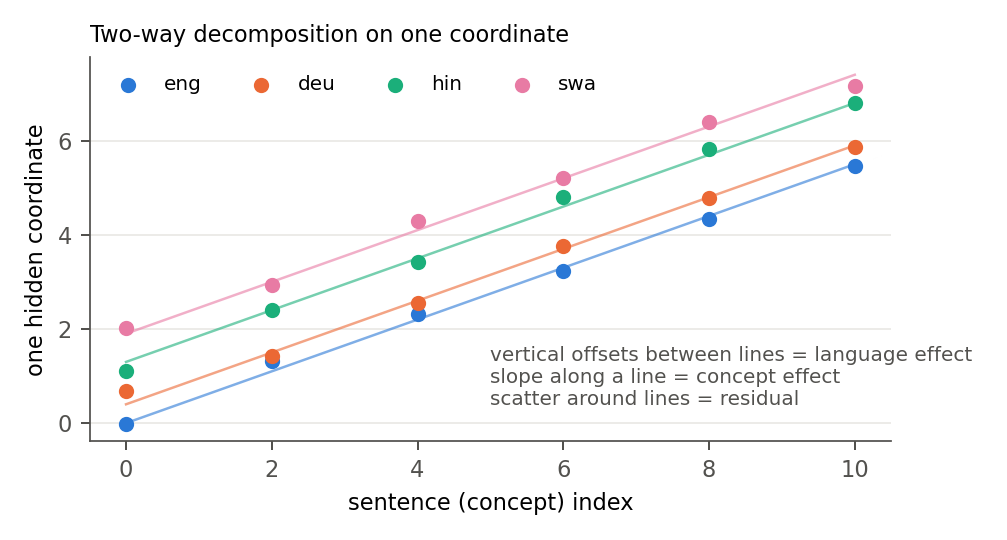
\includegraphics[width=0.8\linewidth]{fig_stats_anova.png}
\caption{One hidden coordinate on a small grid: language offsets, concept slope, residual scatter.}\label{fig:anova}\end{figure}

\textbf{Degrees of freedom} count independent pieces of information:
$L-1$ for languages, $N-1$ for sentences, $(L-1)(N-1)$ for the residual. A
\emph{mean square} is a sum of squares divided by its degrees of freedom.

\textbf{Expected mean squares and variance components.} If the effects are
random with variances $\sigma^2_L$, $\sigma^2_C$ and noise $\sigma^2_E$, then
$\mathbb E[\mathrm{MS}_L] = \sigma^2_E + N\sigma^2_L$,
$\mathbb E[\mathrm{MS}_C] = \sigma^2_E + L\sigma^2_C$,
$\mathbb E[\mathrm{MS}_E] = \sigma^2_E$. Solving gives noise-corrected
estimates of each component (the method of moments); restricted maximum
likelihood (REML) does the same with a non-negativity constraint. This is
the LFS-VC variant in the paper. The pure-noise value of the direct LFS
estimator follows from the same expectations with $\sigma^2_L =
\sigma^2_C = 0$: $(L-1)/(L+N-2)$.

\begin{exercise}{verify the decomposition and the null by simulation}
\begin{lstlisting}
def two_way(X):                       # X: (L, N, D)
    L, N, D = X.shape; mu = X.mean((0, 1)); ml = X.mean(1); mc = X.mean(0)
    ss_l = N * ((ml - mu)**2).sum(); ss_c = L * ((mc - mu)**2).sum()
    ss_r = ((X - ml[:, None] - mc[None] + mu)**2).sum(); tot = ((X - mu)**2).sum()
    return ss_l, ss_c, ss_r, tot
X = rng.normal(size=(12, 120, 64))
ss_l, ss_c, ss_r, tot = two_way(X)
print(abs(ss_l + ss_c + ss_r - tot))                    # ~1e-9: exact identity
lfs = [two_way(rng.normal(size=(12, 120, 64)))[0] for _ in range(50)]
sim = np.mean([a / (a + two_way(rng.normal(size=(12,120,64)))[1]) for a in lfs])
print(sim, 11 / (11 + 119))                              # both ~0.0846
\end{lstlisting}
Then add a language effect (\texttt{X += rng.normal(0, 0.5, (12,1,64))}) and
watch the share rise; add a concept effect and watch it fall.
\end{exercise}

\subsection{Standardization and invariances}

Z-scoring a coordinate subtracts its mean and divides by its standard
deviation, an affine map. Done jointly over all cells, it equalizes
coordinate variances without touching the language or sentence structure
within a coordinate. LFS is then invariant to uniform rescaling of all
vectors, to any positive rescaling of individual coordinates, and to
rotations of the coordinate basis; it is \emph{not} invariant to the choice
of basis before standardization (whitening changes it), to pooling, or to
the grid size. Every one of those was measured, and each dictates a
reporting rule.

\subsection{Correlation}

Pearson's $r$ measures linear association; Spearman's $\rho$ is Pearson on
ranks, so it ignores monotone transformations and is robust to outliers. The
paper reports Spearman. A correlation of 0.5 explains a quarter of the
variance; 0.9 explains 81 percent. Correlation is symmetric and says nothing
about cause.

\subsection{Confounding, residualization, and the confounder adjustment regression}

If languages with more training data have both higher alignment and higher
accuracy, then the raw correlation between alignment and accuracy is partly
``data size predicting data size''. The remedy is to remove the observables
from both variables and correlate what is left (Figure~\ref{fig:deflation}).

\begin{figure}[h]\centering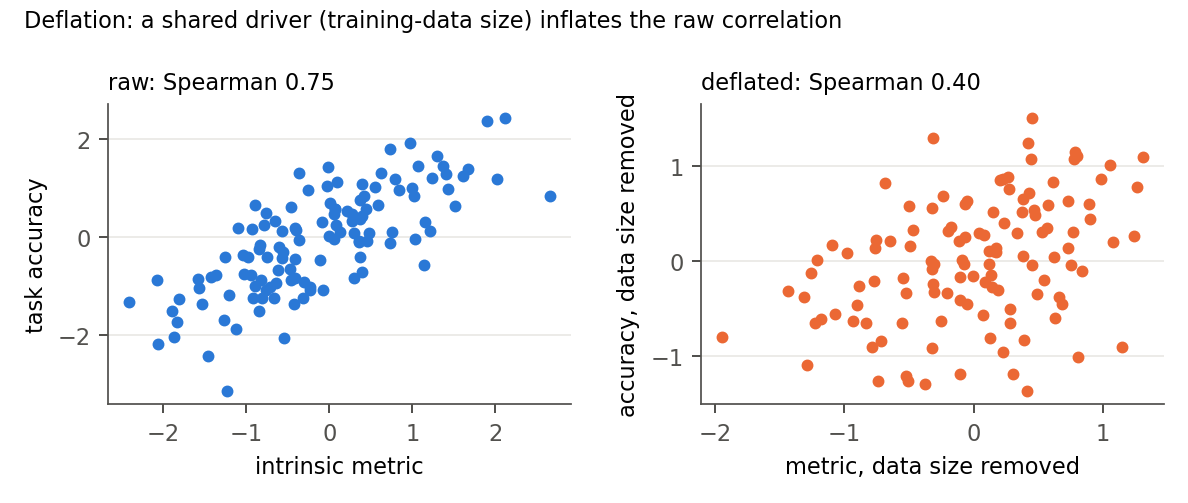
\includegraphics[width=0.9\linewidth]{fig_stats_deflation.png}
\caption{Synthetic illustration: a shared driver inflates the raw correlation; residualizing on it leaves the genuine incremental relationship.}\label{fig:deflation}\end{figure}

The paper's regression, for each (model, language) cell:
\[
\mathrm{logit}\!\Big(\tfrac{\mathrm{acc}-0.25}{0.75}\Big) = \text{model FE} + \beta_1 \log_{10}(\text{tokens}) + \beta_2\,\text{macro-family} + \beta_3\,\text{script} + \beta_4\,\text{fertility} + \alpha .
\]
Three details to be able to explain. The \emph{logit transform above the
chance floor} maps accuracies in $(0.25, 1)$ onto the real line so that
differences near the floor and near the ceiling are comparable.
\emph{Model fixed effects} (one dummy per model) absorb each model's overall
level, so the comparison is across languages within a model. \emph{Cluster-robust
standard errors by language} account for the fact that the same language
appears once per model. The residual $\alpha$ is the ``transfer residual'';
metric validity is the Spearman correlation between the residualized metric
and $\alpha$. A validity check precedes everything: the token coefficient must be
positive and significant, or the proxy is broken.

\begin{exercise}{residualize and correlate}
Generate \texttt{tokens}, a \texttt{metric} that depends on tokens plus noise,
and an \texttt{acc} that depends on tokens and a little on the metric.
Compute Spearman raw; then regress both on tokens, take residuals, and
compute Spearman again. Vary the ``little'' and watch when the confounder-adjusted
correlation vanishes. This is Figure~\ref{fig:deflation}.
\end{exercise}

\subsection{Uncertainty: bootstrap, clusters, and the unit of generalization}

A confidence interval says how much the estimate would move if you redrew
the sample. The bootstrap estimates that by resampling your own data with
replacement many times and recomputing the statistic. The key choice is
\emph{what to resample}. If you want to generalize to new languages,
resample languages; to new models, resample models; to both, resample both
(crossed). Rows within a model are correlated, so resampling rows overstates
certainty about models (Figure~\ref{fig:bootstrap}). Four models cannot
support a model-level claim because a four-model bootstrap has only a handful
of distinct resamples; nineteen can. This single point is why the R1
expansion was run and why every interval in the paper is reported by unit.

\begin{figure}[h]\centering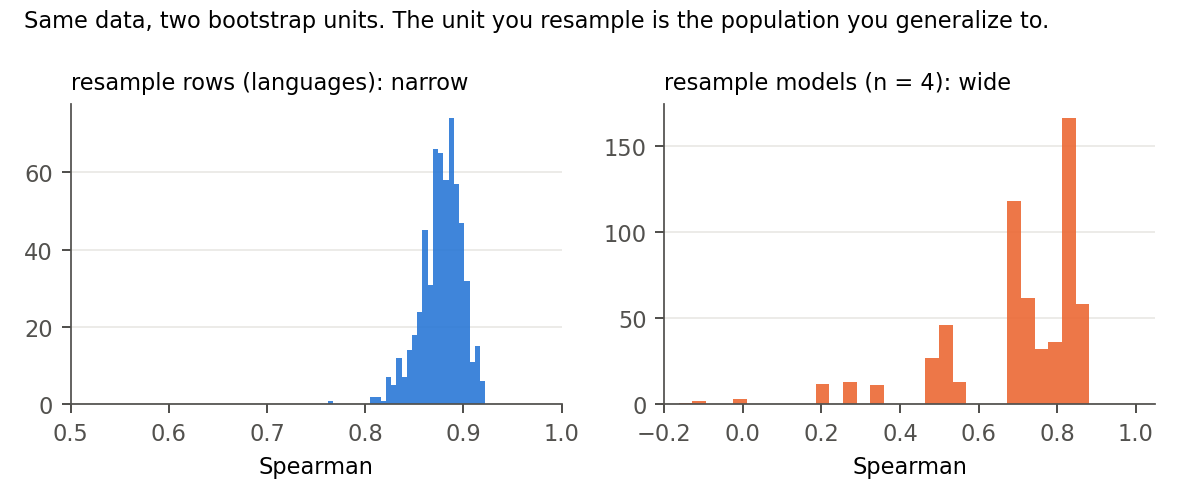
\includegraphics[width=0.9\linewidth]{fig_stats_bootstrap.png}
\caption{Same synthetic data: resampling rows gives a narrow interval; resampling the four models gives a wide one. The second is the right one for a claim about models.}\label{fig:bootstrap}\end{figure}

\emph{Effective sample size.} When 40 languages are highly correlated within
a model, they carry the information of far fewer independent languages
(about 1.2 to 2 in the project's panels). Nominal $n$ overstates evidence;
cluster bootstraps do not.

\emph{Leave-one-out.} Recompute the statistic dropping one family (or model)
at a time. If every estimate stays positive, no single family drives the
result. The content-transfer result stays between 0.44 and 0.60 under
leave-one-family-out.

\begin{exercise}{cluster bootstrap for Spearman}
\begin{lstlisting}
from scipy.stats import spearmanr
def boot_ci(x, y, groups, B=2000):
    ids = np.unique(groups); out = []
    for _ in range(B):
        pick = rng.choice(ids, len(ids), replace=True)
        idx = np.concatenate([np.where(groups == g)[0] for g in pick])
        out.append(spearmanr(x[idx], y[idx]).statistic)
    return np.nanpercentile(out, [2.5, 97.5])
\end{lstlisting}
Build 4 models $\times$ 34 languages with a model-level effect; compare
\texttt{groups = model} against \texttt{groups = language}.
\end{exercise}

\subsection{Multiple comparisons}

Test twenty hypotheses at $p < 0.05$ and one will ``pass'' by chance.
Benjamini--Hochberg adjusts a family of $p$-values to control the false
discovery rate; the paper applies it over its preregistered comparison set.
The deeper protection is preregistration: fewer, named tests.

\subsection{Measurement theory: validity, reliability, Goodhart}

\begin{description}[leftmargin=3.4cm, style=nextline, itemsep=1pt]
\item[construct validity] does the number measure what it claims? Evidence: the exact decomposition, the null, the invariances, the probe contrast, the fault test suite.
\item[predictive validity] does it relate to behavior it should relate to? Evidence: content transfer yes; pooled benchmarks no, with a measured reason.
\item[reliability and ceilings] two independent measurements of the same thing agree at 0.315 on their residuals, so no predictor of one can exceed about $\sqrt{0.315} = 0.56$. Spearman--Brown: averaging parallel forms raises reliability.
\item[Goodhart's law] a measure that becomes a target stops measuring. The Aim 2 reversal is a textbook case; BLEU as a training objective is the MT analogue.
\item[preregistration] write the prediction, criterion, and analysis in a dated file before seeing the outcome, and report every failure. It is why the collapse blind spot can be called ``predicted before observed''.
\item[minimum detectable effect] the smallest effect a design can find; a criterion without one returns verdicts it has no power to support (discrepancy ledger D7).
\end{description}

\subsection{Linear algebra tools, in one paragraph each}

\textbf{PCA and SVD.} Directions of largest variance; the spectrum tells how
many directions matter. \textbf{Effective rank and participation ratio.}
Scalar summaries of that spectrum; they fell by 80 to 90 percent when concept
rank collapsed while LFS moved little. \textbf{Whitening (ZCA).} Rotate
and rescale so the covariance is the identity; it equalizes the spectrum and,
in the paper, collapsed the measured language share for 13 of 14 models,
which is how we know language identity lives in high-variance directions.
\textbf{Procrustes.} The best rotation aligning one point set to another;
the map M3 of the sequence. \textbf{Ridge regression.} Least squares with a
penalty; the hub test and map M4. \textbf{Gini coefficient.} A
concentration measure from 0 (spread evenly) to 1 (all in one place); the
coordinate-energy Gini fell from 0.855 to 0.542 under random rotations,
which is why no ``language neuron'' claim is made.

\clearpage
\section{The Language-Factor Share, end to end}
\label{ch:lfs}

\subsection{The question}

When the same sentence is written in many languages and run through a model,
how much of the model's internal representation at a given layer is organized
by \emph{which language} it is, and how much by \emph{what it means}? LFS
answers with one number in $[0,1]$ per layer: near 1, the vectors cluster by
language whatever the sentence says; near 0, they cluster by meaning whatever
the language. Across layers the numbers form a depth profile.

\subsection{The grid}

Take $N$ sentences that exist in all $L$ languages with the same meaning.
NTREX-128 gives the WMT19 news test set in 128 languages; the profiles use
$N = 300$ and $L = 128$. Every cell (language $l$, sentence $c$) is one
string, and the grid is \emph{balanced}: every language has every sentence.
Balance is what makes the decomposition exact.

\subsection{From strings to vectors}

Run each string through the model with hidden states enabled. At one layer,
average the token vectors over the sentence's real tokens (not padding) in
fp32. That gives one vector $\mathbf h_{lc} \in \R^D$ per cell, and an
$L\times N\times D$ tensor per layer. Layer 0 is the embedding output; layer
$k$ is the residual stream after block $k$ (Chapter~\ref{ch:llm}).

\subsection{Standardize each coordinate, jointly}

For each coordinate $d$, subtract its mean and divide by its standard
deviation, both taken over all $L\times N$ cells together:
\[
z_{lcd} = \frac{h_{lcd} - \overline{h}_{\cdot\cdot d}}{s_d}.
\]
Why: a few coordinates carry values hundreds of times larger than the rest
and would decide the answer alone. Why jointly: standardizing each language
separately would subtract each language's mean, which is the quantity being
measured. After standardization every coordinate has the same total
variance, so LFS becomes a weighted average of per-coordinate language shares
in which no coordinate can dominate by scale.

\subsection{Three averages and two sums of squares}

\begin{figure}[h]\centering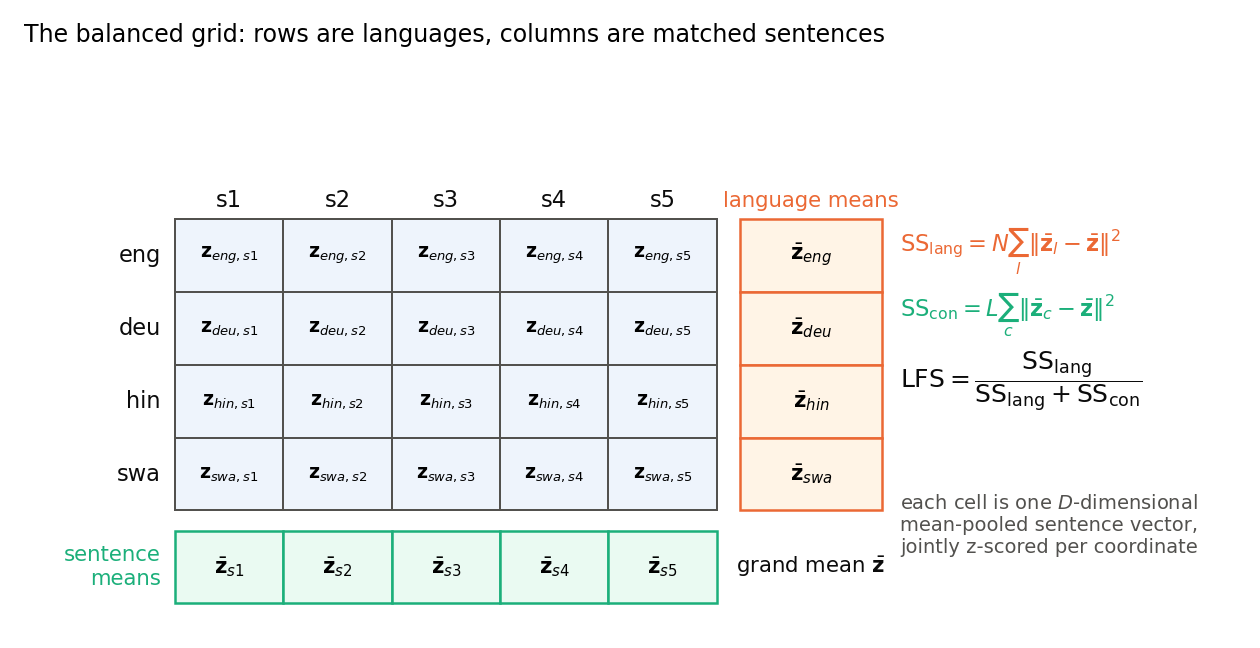
\includegraphics[width=\linewidth]{fig_lfs_grid.png}
\caption{Row means isolate language (they average over meaning); column means isolate meaning (they average over language).}\label{fig:grid}\end{figure}

Compute the grand mean $\bar{\mathbf z}$, the language means $\bar{\mathbf
z}_l$ (average over the $N$ sentences of language $l$), and the sentence means
$\bar{\mathbf z}_c$ (average over the $L$ translations of sentence $c$).
Averaging over sentences within a language cancels meaning and leaves
language identity; averaging over languages within a sentence cancels
language and leaves meaning. Then
\[
\SSl = N\sum_{l}\|\bar{\mathbf z}_l - \bar{\mathbf z}\|^2,\qquad
\SSc = L\sum_{c}\|\bar{\mathbf z}_c - \bar{\mathbf z}\|^2,\qquad
\SSr = \sum_{l,c}\|\mathbf z_{lc} - \bar{\mathbf z}_l - \bar{\mathbf z}_c + \bar{\mathbf z}\|^2,
\]
\[
\LFS = \frac{\SSl}{\SSl + \SSc}.
\]
The multipliers $N$ and $L$ are bookkeeping: each language mean stands for
$N$ cells and each sentence mean for $L$, so with those weights the three
terms add up exactly to the total spread of the grid. The residual is left out
of the ratio because LFS asks how the two \emph{systematic} effects divide; a
noisy model must not look language-agnostic by being noisy. The residual is
reported next to the ratio.

\subsection{A worked example for the whiteboard}

One coordinate, two languages, three sentences:
\begin{center}
\begin{tabular}{lrrr|r}
 & $s_1$ & $s_2$ & $s_3$ & language mean \\ \hline
English & 1.0 & 3.0 & 5.0 & 3.0 \\
German  & 2.0 & 4.0 & 6.0 & 4.0 \\ \hline
sentence mean & 1.5 & 3.5 & 5.5 & grand mean 3.5
\end{tabular}
\end{center}
$\SSl = 3\,[(3.0-3.5)^2 + (4.0-3.5)^2] = 1.5$;\quad
$\SSc = 2\,[(1.5-3.5)^2 + 0 + (5.5-3.5)^2] = 16$;\quad
every residual is zero (check: $1.0 - 3.0 - 1.5 + 3.5 = 0$);\quad
$\LFS = 1.5/17.5 = 0.086$.

Meaning dominates: sentences differ by a lot, languages by a constant
offset of one. Multiply every number by ten: every sum of squares is
multiplied by 100 and the ratio does not move. That is the scale invariance
that later becomes the collapse blind spot. (The REML variant in
\texttt{reports/lfs\_math.pdf} gives 0.11 on the same table because it
subtracts a noise estimate and divides by degrees of freedom; same data,
different estimator. On 14 real models the two rank models identically.)

\begin{exercise}{LFS from scratch, matching the repository code}
\begin{lstlisting}
def lfs(X):                                   # X: (L, N, D), already z-scored per coordinate
    L, N, D = X.shape
    mu = X.mean((0, 1)); mu_l = X.mean(1); mu_c = X.mean(0)
    ss_lang = N * ((mu_l - mu)**2).sum(); ss_con = L * ((mu_c - mu)**2).sum()
    ss_res = ((X - mu_l[:, None] - mu_c[None] + mu)**2).sum()
    return ss_lang / (ss_lang + ss_con), ss_lang, ss_con, ss_res
def zscore(H):                                # H: (L, N, D) raw pooled vectors
    flat = H.reshape(-1, H.shape[-1]); return (H - flat.mean(0)) / (flat.std(0) + 1e-9)
# illustration: language offsets G, concept vectors C, noise E
L, N, D = 12, 300, 128
G = rng.normal(0, 1.0, (L, 1, D)); C = rng.normal(0, 1.5, (1, N, D)); E = rng.normal(0, 0.5, (L, N, D))
H = G + C + E
print(lfs(zscore(H))[0])                       # a share between 0 and 1
print(lfs(zscore(3.7 * H))[0])                 # identical: uniform scale cancels
print(lfs(zscore(C + E))[0], (L-1)/(L+N-2))    # no language effect: near the null
\end{lstlisting}
Compare your function line by line with \texttt{code/pilot\_metrics.py:lfs}
and \texttt{src/analysis/rmfs\_profile.py:factor\_decomposition}. They are
the same estimator.
\end{exercise}

\subsection{What the profile looks like}

\begin{figure}[h]\centering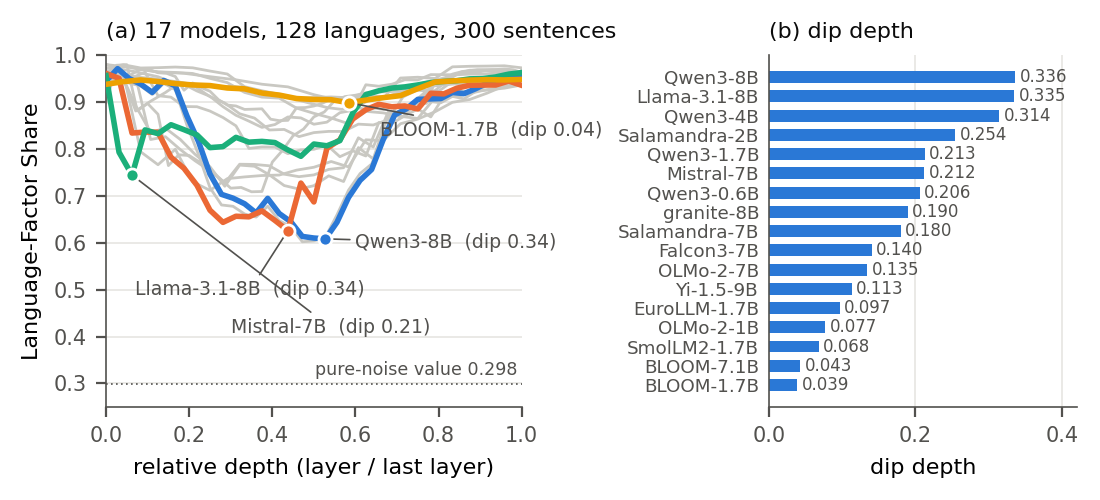
\includegraphics[width=\linewidth]{fig_lfs_profiles_17.png}
\caption{Seventeen models on the 128-language, 300-sentence grid. Left: LFS by relative depth, four models highlighted. Right: dip depth, first-layer value minus minimum.}\label{fig:profiles}\end{figure}

Every one of the 17 primary models and the 19 expansion models has an
interior minimum with both endpoints higher (Figure~\ref{fig:profiles}).
Read it as three stages. Layer 0 is high because the embedding layer knows
the token identity and tokens are language-specific. The interior minimum is
where the model represents the same meaning most similarly across languages;
its depth runs from 0.039 (BLOOM-1.7B) to 0.336 (Qwen3-8B). The rise toward
the output is the model preparing to predict the next token, which is in a
specific language.

Two facts to state before anyone else does. The minimum is above 0.5 for
every model on this grid: even at the most shared layer, language main
effects exceed meaning main effects. Say ``more meaning-weighted relative to
its own endpoints'', never ``concept-dominated''. And the minimum's location
varies: most models place it between 35 and 60 percent depth, but Mistral-7B
(and two continued-pretraining models in the expansion) put a sharp minimum
at layer 2 followed by a plateau.

\begin{figure}[h]\centering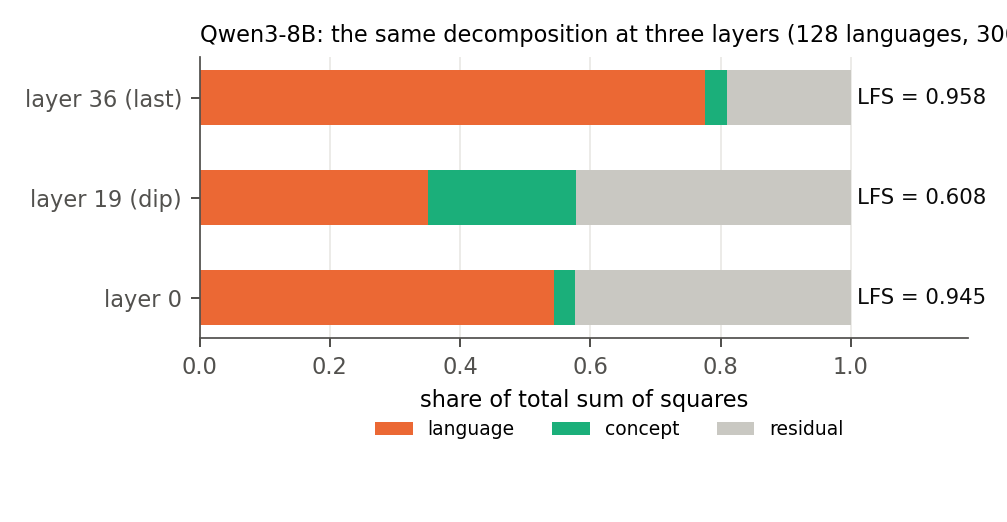
\includegraphics[width=0.8\linewidth]{fig_lfs_decomp.png}
\caption{The same decomposition at three layers of Qwen3-8B. The residual (gray) is never in the ratio but always reported.}\label{fig:decomp}\end{figure}

\subsection{Properties, each with a short proof}

\textbf{Bounded.} Both sums of squares are non-negative, so $\LFS\in[0,1]$.

\textbf{Exact decomposition.} With $a_l = \bar{\mathbf z}_l - \bar{\mathbf
z}$, $b_c = \bar{\mathbf z}_c - \bar{\mathbf z}$, $r_{lc}$ the residual,
$\mathbf z_{lc} - \bar{\mathbf z} = a_l + b_c + r_{lc}$. On a balanced grid
$\sum_l a_l = 0$, $\sum_c b_c = 0$, and residuals sum to zero along every
row and column; expanding the squared norm and summing over the grid, every
cross term contains one of those zero sums. Hence total $=\SSl+\SSc+\SSr$.

\textbf{Uniform-scale invariance.} Multiply every vector by $k$: every sum of
squares is multiplied by $k^2$; the ratio is unchanged. After standardization
LFS is also invariant to any positive rescaling of individual coordinates.
Consequence: LFS cannot see all representations shrinking together
(Figure~\ref{fig:collapse}).

\textbf{Rotation invariance.} A rotation of the coordinate basis preserves
every norm in the sums, so the global LFS is unchanged. Which coordinates
carry the language energy is not invariant; hence no ``language neuron''
claims.

\textbf{The finite-grid null.} With no structure and isotropic noise of
variance $\sigma^2$ in $D$ coordinates, $\mathbb E[\SSl] = (L-1)D\sigma^2$
(language means average $N$ cells; $L-1$ degrees of freedom) and $\mathbb
E[\SSc] = (N-1)D\sigma^2$. Their ratio is
\[
\LFS_{\text{null}} = \frac{L-1}{L+N-2},
\]
independent of $D$: 0.298 at $(128, 300)$, 0.078 at $(128, 1500)$
(Figure~\ref{fig:null}). Three consequences: absolute values are not
comparable across grids, pooling schemes, or granularities; differences at a
fixed grid are fine because the noise term is common; and the null is not a
floor, since strong meaning structure with weak language structure drives
LFS below it. Verified on synthetic noise and on pseudo-language splits of
real representations to three decimals.

\begin{figure}[h]\centering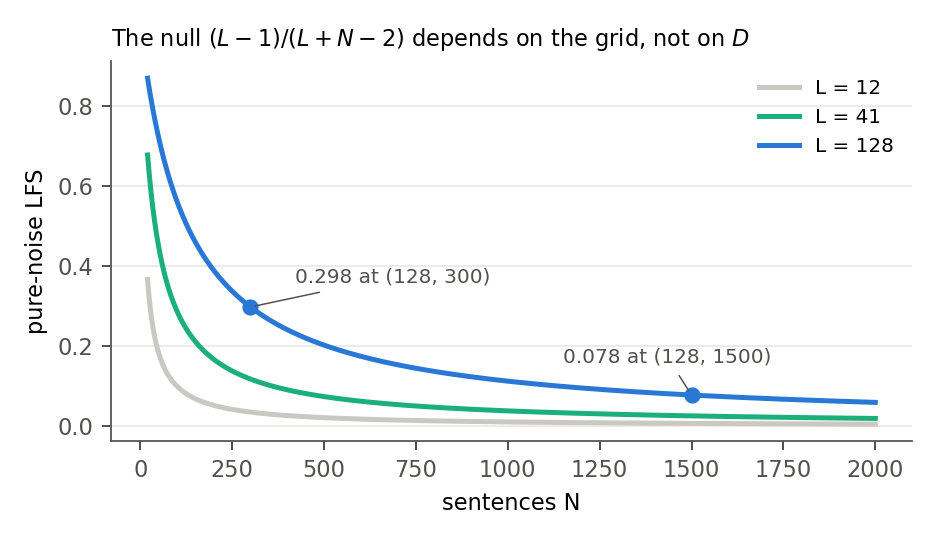
\includegraphics[width=0.7\linewidth]{fig_lfs_null.png}
\caption{The pure-noise value depends on the grid. Compare LFS values only at a fixed grid.}\label{fig:null}\end{figure}

\textbf{Near-independence of evaluation size.} The noise term shrinks as a
share of the numerator as $N$ grows, so LFS drifts by $-0.006$ to $-0.010$
from $N=100$ to $N=1000$; a retrieval score moves $-0.065$ to $-0.125$ on the
same draws. This is the practical argument for LFS over retrieval scores when
comparing across studies.

\textbf{Differentiable.} LFS is a smooth function of the vectors, so it can
be a loss. That made the Aim 2 test possible; the test showed it should not be
one.

\subsection{The boundary and the failure mode}

LFS measures the \emph{additive} language component: how far each language's
mean sits from the center. Rotations, warps, and language-by-meaning
interactions land in the residual. The misalignment decomposition measured how much
that matters: offset plus scale explain 63 to 97 percent of held-out
cross-language misalignment, rotation under one percent, with the instrument
recovering injected rotations exactly. Language identity nonetheless stays
linearly decodable at every layer (probe accuracy 0.875 to 0.886, chance
0.042): variance share and separability are different quantities.

\begin{figure}[h]\centering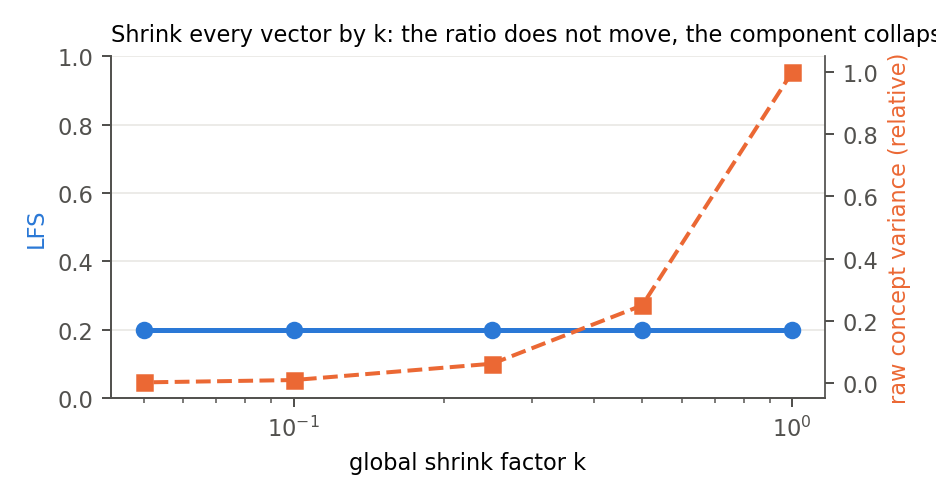
\includegraphics[width=0.7\linewidth]{fig_lfs_collapse_synthetic.png}
\caption{Synthetic collapse: shrink every vector and the ratio is flat while the raw concept component vanishes.}\label{fig:collapse}\end{figure}

\begin{figure}[h]\centering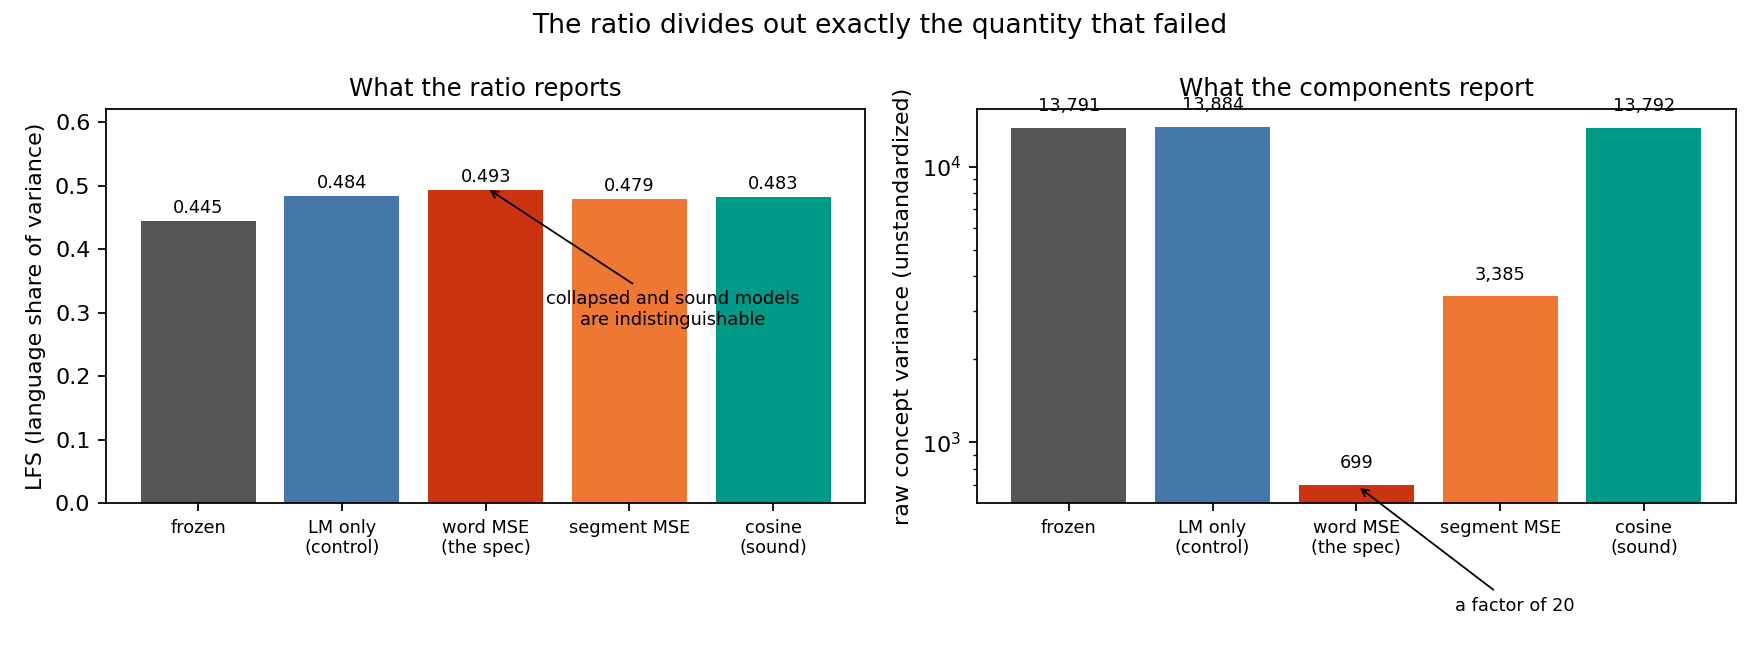
\includegraphics[width=\linewidth]{fig_lfs_collapse_trained.png}
\caption{The same thing in a trained model. The word-MSE condition lost 95 percent of raw concept variance; LFS moved by 0.05 and MEXA ranked it first.}\label{fig:collapse_trained}\end{figure}

Own this before anyone raises it: in the Aim 2 word-alignment condition the
representation norm fell from 451 to 42 and raw concept variance from 13{,}791
to 699 while LFS moved from 0.445 to 0.493 and the retrieval metric ranked the
collapsed model first (Figure~\ref{fig:collapse_trained}). Every
scale-invariant measure shares this blind spot, by theorem. The fix is to
report the ratio with its raw components ($\SSl$, $\SSc$, residual, norm), so
that collapse shows up where it lives.

\subsection{What LFS relates to, and what it does not}

\begin{figure}[h]\centering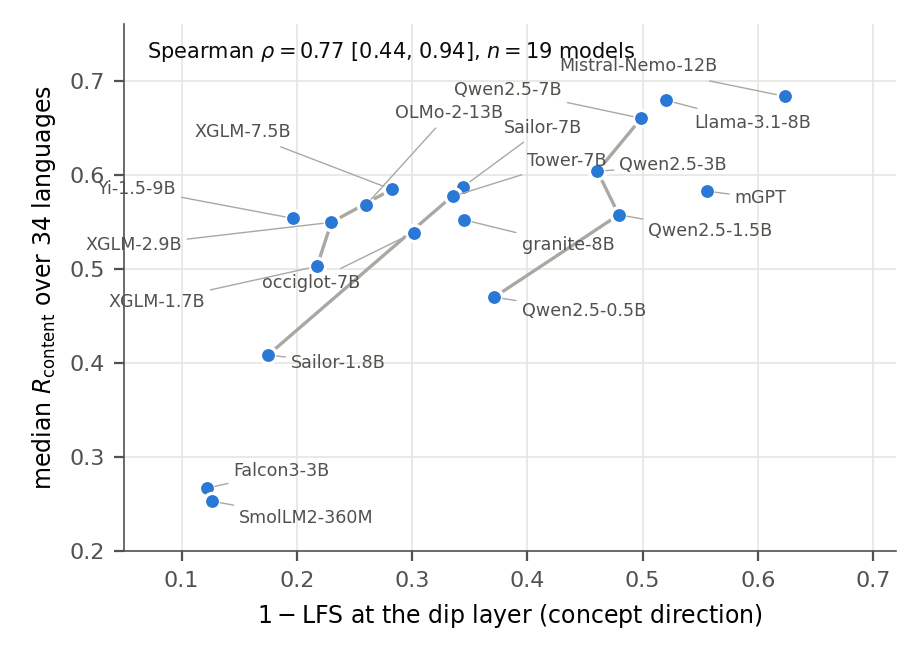
\includegraphics[width=0.66\linewidth]{fig_r1_model_level.png}
\caption{Nineteen models: sentence-component share ($1-$LFS-VC) at the dip against median content transfer. Spearman 0.77 at the model level; 0.51 [0.19, 0.71] on the full confounder-adjusted panel.}\label{fig:r1}\end{figure}

\textbf{Content transfer (positive).} Give a model an English sentence to
predict, preceded by the previous sentence of the same document in another
language, versus a wrong-document sentence in that language; the improvement
from the right context is the content benefit. Across 19 models and 13
families, models with a more meaning-weighted dip layer show more content
transfer after controlling for data exposure, family, script, and fertility
(Figure~\ref{fig:r1}).

\textbf{Benchmark accuracy (null).} Against pooled multiple-choice accuracy on 33
models, LFS has no association once exposure is removed (0.04, interval
crossing zero); MEXA reaches 0.24. Two independent benchmarks agree on only about a
third of their per-language residual variation, which caps what any intrinsic
metric can predict there.

\textbf{Training objective (negative).} Minimizing LFS deepens the dip
quickly but through a shortcut that damages alignment and capability; across
18 trained condition-seed points lower LFS went with worse tail alignment. LFS is a
measurement, not a target.

\subsection{The family}

LFS answers one question. The other questions a multilingual representation
raises are answered by accompanying measures on the same grid, each validated on
its own question and never averaged into a single score:

\begin{center}\small
\begin{tabular}{p{4.6cm}p{5.2cm}p{4.6cm}}
\toprule
Question & Measure & Exposes \\
\midrule
Language vs.\ meaning share, per layer & LFS profile; dip depth & structure; recipe differences \\
Did scale or concept variance collapse? & raw $\SSl$, $\SSc$, residual, norm vs.\ a frozen reference & collapse a ratio hides \\
Is the cross-language map simple? & nested maps M0--M5, held-out error reduction & additive vs.\ rotational vs.\ nonlinear \\
Is the shared factor English? & latent-factor vs.\ English donor $R^2$ & English-centricity \\
Do the hardest sentences align? & AaR@10, worst-decile margin & tail failures that means hide \\
\bottomrule
\end{tabular}
\end{center}

MEXA is the published reference measure, not a family member. The proposal's own list
of candidate metric types (raw distances; mapping complexity; ``anything else
that emerges'') maps onto this table.

\subsection{How to say it}

\say{\textbf{Ten seconds.} LFS measures, at each layer, how much of the
systematic variation in a model's hidden states follows the language of a
sentence rather than its meaning, on a grid of matched translations.}

\say{\textbf{Thirty seconds.} Take the same 300 sentences in 128 languages,
run them through the model, and average token states into one vector per
sentence per language. Standardize coordinates jointly. The spread of the
language means measures language; the spread of the sentence means measures
meaning; LFS is the first divided by the sum. Across 33 models it falls to an
interior minimum and recovers, and how far it falls varies nine-fold and
tracks training recipe more than size. It must be reported with its raw
components, because the ratio cannot see everything shrinking at once.}

\say{\textbf{Two minutes.} Add: the exact two-way decomposition and why the
residual is excluded; the null $(L-1)/(L+N-2)$ and fixed-grid comparison;
values above 0.5 read relatively; the additive boundary measured at under one
percent rotation; the multilingual latent factor beating English in 113 to
124 of 127 languages; content transfer on 19 models at 0.51 [0.19, 0.71];
pooled benchmarks null with a measured ceiling; the collapse case; the family of
measures and the rule against averaging them.}

\clearpage
\section{What the numbers actually look like}
\label{ch:numbers}

The two-language, three-sentence table in Chapter~\ref{ch:lfs} is made up. It
is the smallest object on which the arithmetic can be shown. This chapter
shows the real object, taken from the saved hidden states of Qwen3-8B-Base on
7 September 2026 with the same function the paper's bootstrap uses
(\texttt{lfs\_components} in \texttt{src/analysis/dip\_bootstrap.py}; the
extraction script is \texttt{hidden\_slice.py}, run on the CLSP cpu partition).

\begin{figure}[h]\centering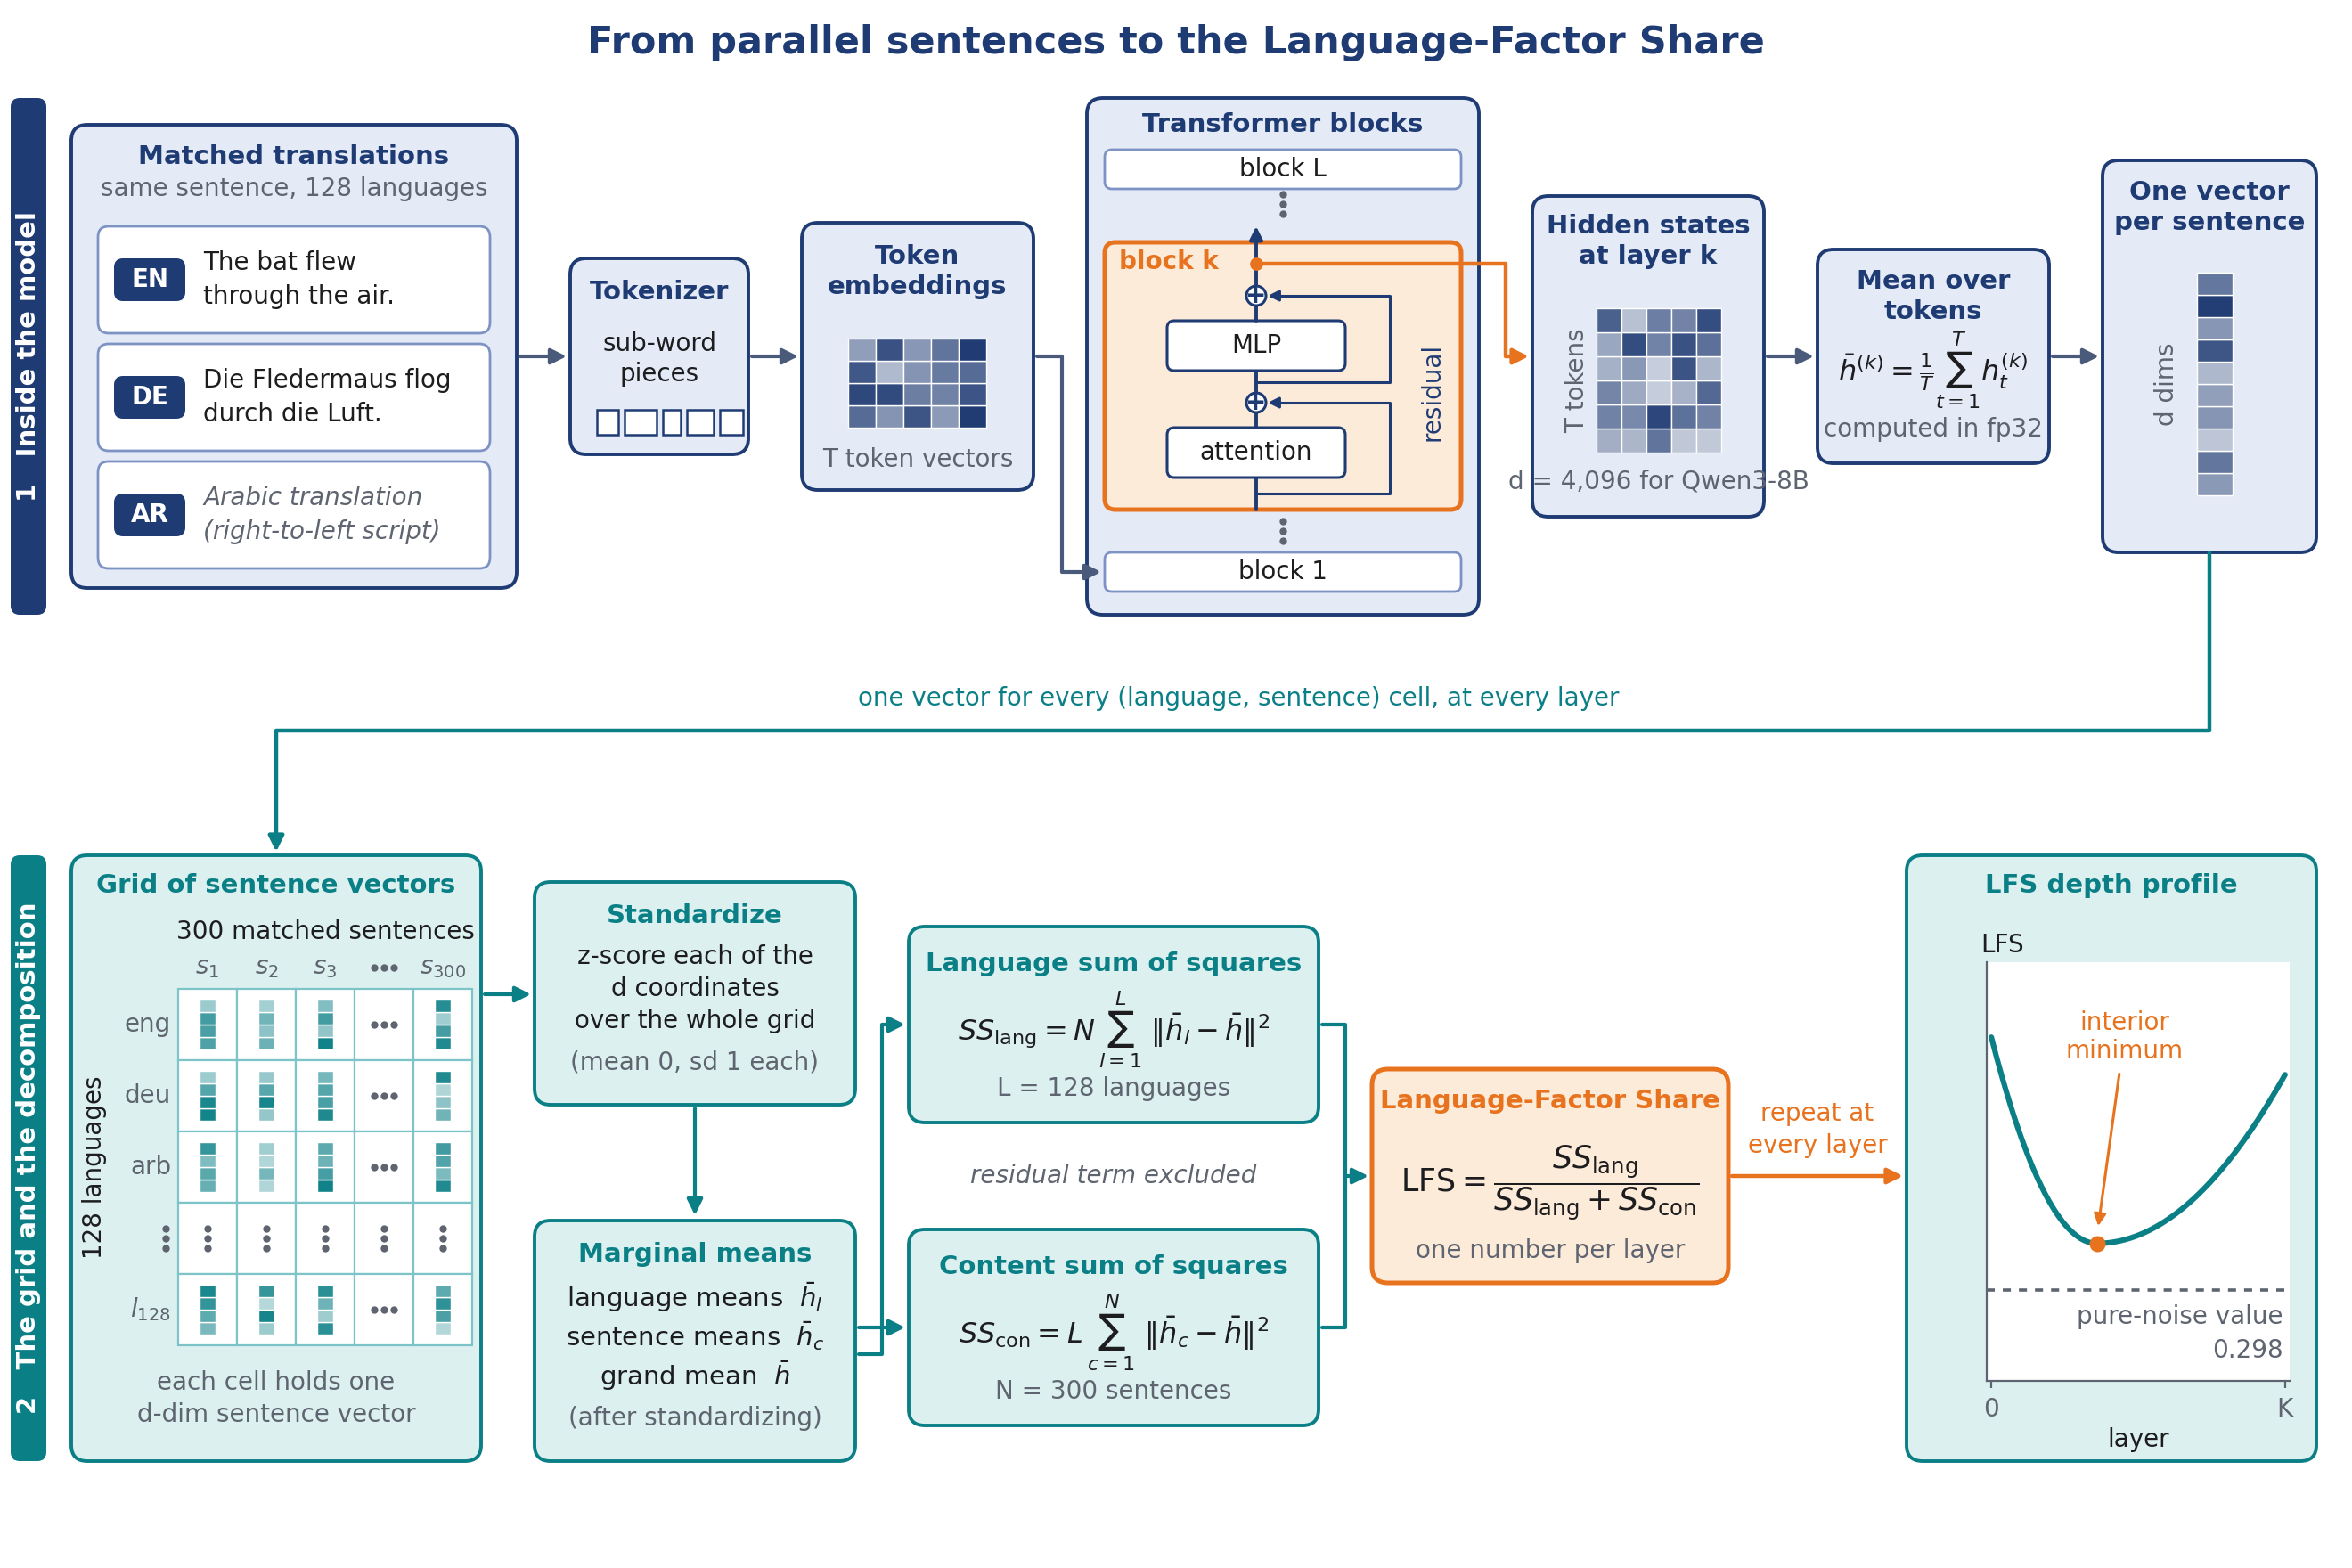
\includegraphics[width=\linewidth]{figs/report/fig22_pipeline_diagram.png}
\caption{The whole measurement on one page: inside the model (top) and the grid with its decomposition (bottom).}\label{fig:pipeline-guide}\end{figure}

\subsection{The table is a three-dimensional array}

Nothing is ever typed into a table. After the forward pass, mean pooling over
tokens gives one vector per (language, sentence) pair. Stacked, they form an
array
\[
X[\ell, c, d], \qquad \ell = 1..128 \text{ languages},\; c = 1..300 \text{ sentences},\; d = 1..4096 \text{ coordinates},
\]
one such array per layer. The example in Chapter~\ref{ch:lfs} is this array
with $L=2$, $N=3$, $D=1$. Everything below is the same array with the real
sizes. Stored on the cluster as \texttt{layer000.npz}, \texttt{layer019.npz},
and so on; the first 300 of the 1,500 stored sentences are the main grid.

\subsection{Raw values at the dip layer}

Table~\ref{tab:rawvals} shows the first five of the 4,096 coordinates for
three sentences in seven languages at layer 19, the dip layer of Qwen3-8B.
These are the numbers the model produced, mean-pooled, before any
standardization. Two things to notice. They are ordinary floating-point
numbers, mostly between $-1$ and $1$. And a language does not announce
itself: nothing in the Arabic rows looks obviously different from the English
rows on these five coordinates. The language effect is spread thinly over
thousands of coordinates and only becomes visible when you average.

\begin{table}[h]\centering\small
\caption{Qwen3-8B-Base, layer 19, mean-pooled hidden states, coordinates 0 to 4.}
\label{tab:rawvals}
\begin{tabular}{llrrrrr}
\toprule
Language & Sentence & $d_0$ & $d_1$ & $d_2$ & $d_3$ & $d_4$ \\
\midrule
eng & 0 & 0.159 & 0.191 & $-0.902$ & 0.012 & 0.651 \\
eng & 1 & $-0.085$ & $-0.811$ & $-0.418$ & $-0.140$ & 0.448 \\
eng & 2 & $-0.928$ & 0.185 & $-0.486$ & $-0.369$ & 0.076 \\
deu & 0 & $-0.236$ & 0.287 & $-0.567$ & $-0.213$ & 0.385 \\
deu & 1 & $-0.453$ & $-0.218$ & $-0.384$ & 0.205 & 0.245 \\
deu & 2 & $-0.439$ & $-0.165$ & $-0.909$ & $-0.071$ & 0.292 \\
fra & 0 & $-0.311$ & $-0.036$ & $-1.171$ & $-0.149$ & 0.051 \\
fra & 1 & $-0.667$ & $-0.311$ & $-0.713$ & $-0.038$ & $-0.171$ \\
fra & 2 & $-0.325$ & $-0.646$ & $-1.328$ & $-0.203$ & $-0.028$ \\
spa & 0 & 0.185 & $-0.504$ & $-0.142$ & 0.032 & 0.064 \\
spa & 1 & $-0.060$ & $-0.774$ & $-0.538$ & 0.124 & 0.112 \\
spa & 2 & $-0.662$ & $-0.279$ & $-1.328$ & 0.145 & $-0.014$ \\
rus & 0 & $-0.207$ & $-0.119$ & $-0.102$ & $-0.014$ & 0.190 \\
rus & 1 & $-0.406$ & $-0.288$ & $-0.161$ & 0.134 & 0.202 \\
rus & 2 & $-0.472$ & $-0.686$ & $-0.541$ & $-0.232$ & 0.210 \\
arb & 0 & $-0.308$ & 0.533 & $-0.108$ & 0.359 & $-0.130$ \\
arb & 1 & $-0.255$ & $-0.182$ & $-0.117$ & 0.415 & 0.001 \\
arb & 2 & $-0.026$ & $-0.048$ & $-0.706$ & 0.257 & $-0.164$ \\
fas & 0 & 0.067 & 0.434 & $-0.257$ & 0.434 & 0.382 \\
fas & 1 & $-0.469$ & 0.403 & $-0.400$ & 0.860 & 0.151 \\
fas & 2 & $-0.259$ & 0.778 & $-0.703$ & 0.540 & $-0.094$ \\
\bottomrule
\end{tabular}
\end{table}

\subsection{The table on one coordinate, with real means}

Fix one coordinate and the array becomes exactly the Chapter~\ref{ch:lfs}
table, 128 rows by 300 columns. Table~\ref{tab:onecoord} shows coordinate
1082 at layer 19, a coordinate of typical spread, for the seven languages and
three sentences, together with the three kinds of mean:

\begin{itemize}[leftmargin=1.6cm]
\item[language mean] the mean of that language's row over all 300 sentences
(the ``column mean'' of the small example, where languages were columns);
\item[sentence mean] the mean of that sentence's column over all 128
languages;
\item[grand mean] the mean of all $128 \times 300 = 38{,}400$ cells.
\end{itemize}

\begin{table}[h]\centering\small
\caption{Coordinate 1082, layer 19. Values for three sentences, then each language's mean over all 300 sentences. The sentence means are over all 128 languages.}
\label{tab:onecoord}
\begin{tabular}{lrrrr}
\toprule
Language & sentence 0 & sentence 1 & sentence 2 & language mean (300 sentences) \\
\midrule
eng & 0.209 & 0.315 & 0.759 & 0.155 \\
deu & 0.369 & 0.413 & 0.841 & 0.207 \\
fra & 0.406 & 0.483 & 0.587 & 0.220 \\
spa & 0.142 & 0.186 & 0.657 & 0.240 \\
rus & 0.554 & 0.120 & 0.346 & 0.121 \\
arb & 0.210 & 0.453 & 0.401 & 0.321 \\
fas & 0.445 & 0.528 & 0.606 & 0.274 \\
\midrule
sentence mean (128 languages) & 0.148 & 0.244 & 0.323 & grand mean 0.181 \\
\bottomrule
\end{tabular}
\end{table}

On this single coordinate the language sum of squares is
$300 \sum_\ell (\bar x_\ell - \bar x)^2 = 637.9$ and the sentence sum of
squares is $128 \sum_c (\bar x_c - \bar x)^2 = 634.5$, so the language share
of this coordinate is $0.501$. That is one coordinate's vote.

\subsection{``Coordinate by coordinate'' means 4,096 such tables}

LFS does not pick one coordinate. It computes the two sums of squares on
every coordinate and adds them up. In vector form that is what
$\|\bar{\mathbf z}_\ell - \bar{\mathbf z}\|^2$ does: a squared norm is a sum
over coordinates of squared differences, so the language sum of squares of
the whole grid is the sum of the 4,096 per-coordinate language sums of
squares. The code never builds 4,096 tables; it takes means along the axes of
the array (\texttt{X.mean(1)} for language means, \texttt{X.mean(0)} for
sentence means, \texttt{X.mean((0,1))} for the grand mean) and sums the
squared differences over the coordinate axis.

\subsection{Why standardizing first is not optional}

Here is what the raw array looks like at layer 19 before standardization.
The median coordinate has a standard deviation of $0.26$ across the 38,400
cells. Coordinate 2276 has a mean of $224$ and a standard deviation of
$162$. It is a massive activation, a single coordinate the model uses as an
internal bias that is hundreds of times larger than everything else. Its
values for the same seven languages are in Table~\ref{tab:massive}.

\begin{table}[h]\centering\small
\caption{Coordinate 2276, layer 19, the largest-spread coordinate. Same layout as Table~\ref{tab:onecoord}.}
\label{tab:massive}
\begin{tabular}{lrrrr}
\toprule
Language & sentence 0 & sentence 1 & sentence 2 & language mean \\
\midrule
eng & 718.0 & 315.8 & 450.3 & 454.9 \\
deu & 407.0 & 203.8 & 263.5 & 298.8 \\
fra & 308.8 & 221.8 & 337.5 & 299.1 \\
spa & 237.8 & 208.5 & 398.3 & 309.4 \\
rus & 339.3 & 134.4 & 285.3 & 249.5 \\
arb & 287.3 & 215.1 & 355.5 & 288.8 \\
fas & 265.3 & 200.0 & 235.9 & 200.8 \\
\midrule
sentence mean & 304.0 & 174.3 & 249.0 & grand mean 224.4 \\
\bottomrule
\end{tabular}
\end{table}

Because sums of squares grow with the square of the scale, this one
coordinate carries $92.8$ percent of the total sum of squares of the whole
layer; the top ten coordinates carry $96.5$ percent; the other 4,086
coordinates share the remaining few percent. If LFS were computed on the raw
array, the language sum of squares would be $89.7$ percent coordinate 2276
and the sentence sum of squares $94.9$ percent coordinate 2276, and the
result, $0.347$, would be the language share of one neuron (on its own that
coordinate's share is $0.334$). The other 4,095 coordinates would be
outvoted. That is what ``a single huge dimension dominates'' means: the
metric silently becomes a measurement of whatever that coordinate does,
which here is mostly a bias term with some content in it.

Standardization divides each coordinate by its own standard deviation across
the grid. After that, coordinate 2276 carries $0.02$ percent of the language
sum of squares and $0.06$ percent of the sentence sum of squares, in line
with the $0.024$ percent a coordinate would carry if all were equal, and the
layer-19 LFS is $0.608$. The standardized values are unit-scale numbers: the
English sentence 0 becomes $[1.32, 0.08, -2.41, -0.39, 2.07]$ on the first
five coordinates.

At layer 0 the same check shows why the effect is layer-dependent. There, the
largest coordinate carries $0.8$ percent of the total, the raw and
standardized LFS are $0.929$ and $0.945$, and the mean vector norm is $0.5$.
By layer 19 the mean norm is $240$, a five-hundred-fold growth through the
network, almost all of it in a handful of coordinates. This is the same fact
behind the collapse blind spot in the paper: the raw scale of a
representation is information, and a ratio throws it away, so the components
and the norm are reported beside the ratio.

\begin{exercise}{watch one coordinate take over}
\begin{lstlisting}
import numpy as np
rng = np.random.default_rng(0)
L, N, D = 8, 50, 64
lang = rng.normal(0, 1.0, (L, 1, D)); sent = rng.normal(0, 1.5, (1, N, D))
X = lang + sent + rng.normal(0, 0.5, (L, N, D))    # additive grid, language weaker than content
def lfs(X):
    mu = X.mean((0, 1)); ml = X.mean(1); mc = X.mean(0)
    ssl = X.shape[1] * ((ml - mu)**2).sum(); ssc = X.shape[0] * ((mc - mu)**2).sum()
    return ssl / (ssl + ssc)
def z(X):
    f = X.reshape(-1, X.shape[-1]); return (X - f.mean(0)) / (f.std(0) + 1e-9)
print(round(lfs(X), 3), round(lfs(z(X)), 3))          # similar: no dominant coordinate yet
X[..., 7] += 200 + 160 * rng.normal(size=(L, N))      # one massive coordinate: a per-cell bias, no language structure
print(round(lfs(X), 3), round(lfs(z(X)), 3))          # raw LFS collapses toward that coordinate's own share; standardized LFS barely moves
\end{lstlisting}
Then compute the fraction of the total sum of squares that coordinate 7
carries before and after \texttt{z}. You have reproduced the layer-19
situation of Table~\ref{tab:massive}.
\end{exercise}

\subsection{So, is a table always built?}

Yes, in the only sense that matters: every LFS number in the paper and the
report comes from an array of exactly this shape, languages by sentences by
coordinates, at one layer, standardized coordinate by coordinate, decomposed
into a language part, a sentence part, and a remainder. The grids differ in
size (128 by 300 for the main profiles, 128 by 1,500 for the study
dumps, 116 by 300 for FLORES-200) and in the model, layer, and pooling, but
never in shape or in the arithmetic.

\clearpage
\section{The defense: questions and answers}
\label{ch:defense}

Answers you can give without notes. Every number is the audited one; the
source is \texttt{docs/AIM1\_ASSESSMENT\_FOR\_ICLR\_2026-09-04.md} and the
claims ledger in \texttt{paper/iclr2027/claims\_ledger.csv}.

\subsection*{On the construct}

\textbf{Isn't this just two-way ANOVA on embeddings?}
Yes, the decomposition is standard. The contribution is what is done with it:
a balanced translation grid that makes it exact, a closed-form null that
makes values interpretable, 33 models showing the shape is universal and the
depth nine-fold variable, confounder-adjusted behavioral validation, and stress tests
that show exactly when the ratio misleads. Nobody had done the last three for
any intrinsic multilinguality metric.

\textbf{The U-shape is known.}
Qualitatively, and the paper cites that work. New is the number: a comparable
depth from 0.04 to 0.34 that tracks recipe over scale; the dip is not a
scaling proxy (Salamandra shallows from 2B to 7B while alignment improves);
script and meaning leave on different schedules; and three models put the
minimum at layer 2, which no ``middle layers are shared'' summary predicts.

\textbf{Why is LFS above 0.5 even at the dip?}
With 128 languages the language offsets (script, tokenizer, high-variance
directions) are large relative to the spread of 300 sentence means, and the
numerator carries a noise term that never vanishes. The measure is relative:
the dip layer is more meaning-weighted than the model's own endpoints, and
0.6 is far above the 0.298 null.

\textbf{Why standardize, and why jointly?}
A few coordinates carry values hundreds of times larger than the rest and
would decide the answer alone. Jointly, because per-language standardization
subtracts the language means we are measuring. The whitened variant is also
reported, so the basis choice is disclosed.

\textbf{Why is the residual outside the denominator?}
LFS asks how the two systematic main effects divide. With the residual in
the denominator a noisy model would look language-agnostic. The residual is
reported beside the ratio, and it is where rotations and interactions would
show.

\textbf{Does low LFS mean a universal interlingua?}
No. It means less language-associated variance relative to matched-sentence
variance under this estimator. Language stays decodable by a probe at every
layer.

\subsection*{On comparisons}

\textbf{Why not just use MEXA?}
Different question. MEXA asks whether a sentence's translation is its nearest
neighbor among candidates, against an English pivot. LFS asks how the
variance splits between language and meaning, with no pivot, a closed-form
null, evaluation-size stability where retrieval moves ten times more, and
components that catch a collapse MEXA scored higher on. On pooled benchmark accuracy
neither does well after removing exposure and MEXA is somewhat better; that
is reported. The paper measures structure; it does not compete on a
leaderboard.

\textbf{Then what is LFS for?}
Three uses, all demonstrated: describing where in a model meaning is shared
and comparing models on it; predicting a specific behavior, cross-lingual
content use, across 19 models after controls; and monitoring training, where
its components expose failures that alignment scores miss. Its role in
training is design, monitoring, and evaluation, not the loss.

\subsection*{On the data}

\textbf{Mean pooling injects length and tokenizer effects.}
Measured. Absolute depth moves 0.13 to 0.20 across four pooling schemes;
ordering changes by at most one adjacent swap; the within-family result holds
for two Qwen3 sizes sharing a tokenizer; fertility correlates with each
language's contribution at $+0.42$ to $+0.64$ and is said so.

\textbf{Your data is translated from English on both sides.}
Tested on WMT19 in both directions: level shifts small ($+0.02$ to $+0.06$
language share), ordering preserved at 0.99. The natively authored benchmark gave
the same null as the translated benchmark restricted to the same languages, so the
null is about the narrow resource range of benchmark languages, not translation.

\textbf{Only 300 sentences?}
Profiles use 300 per language and 128 languages; the null is stated for that
grid. The 1,500-sentence study gives the same picture, and LFS drifts by
under 0.01 between 100 and 1,000 sentences.

\textbf{Only Qwen drives this.}
Leave-one-family-out estimates stay between 0.44 and 0.60 for content
transfer; the family bootstrap excludes zero; 13 families are on the panel.

\subsection*{On what it means}

\textbf{Is the dip causal? Does a deeper dip make a model better?}
No causal claim. Across pretrained models a deeper dip goes with more
cross-lingual content use after controls, on 19 models; under intervention
the association reversed. Observation and intervention are different
questions and both are reported.

\textbf{Can I train with it?}
Not by itself. Minimizing LFS finds a shortcut; the proposal's word-level
alignment loss collapsed representations by a factor of twenty while LFS
barely moved and MEXA rose for the collapsed model. Training use needs
the raw components as constraints and independent capability checks.

\textbf{Why not one number per model?}
Because the measures disagree in exactly the cases that matter: a collapsed
model has a fine ratio and a collapsed raw component. A composite was
preregistered and failed its own crash test. The deliverable is a profile
plus a behavioral check chosen for the question.

\textbf{What about instruction-tuned models, other corpora, larger models?}
Open and cheap: FLORES-200 replication, instruct-versus-base pairs, and a
bootstrap on dip depth are forward-pass or CPU experiments listed in
\texttt{docs/AIM1\_NEXT\_EXPERIMENTS\_2026-09-05.md}.

\textbf{What would change your mind?}
A model with a deep dip and poor content transfer after controls at scale; a
corpus on which the profile shape fails; a pooling scheme that breaks the
cross-model ordering. All three were looked for.

\textbf{The one-sentence claim.}
LFS is a reproducible layerwise decomposition of language and concept
structure in multilingual representations whose profile generalizes across 33
models and carries target-specific behavioral signal, and whose measured
limits show why it must be reported with its raw components rather than used
as a score or a loss.

\clearpage
\section{How to read every graph}
\label{ch:figures}

Every figure in the ICLR draft and the technical report, with the same four
questions asked of each: what is on the axes, what one mark is, what to look
for, and the sentence you should be able to say about it. Figures are shown
small here; the full-size versions are in the documents. Read a graph in this
order: axes first, then one mark, then the pattern, then the caption's claim,
and check that the pattern supports the claim.

\subsection{The two figures in the ICLR paper}

\begin{figure}[h]\centering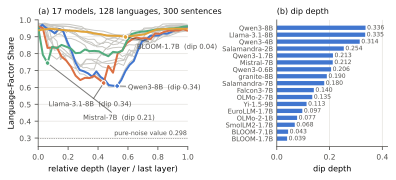
\includegraphics[width=0.95\linewidth]{figs/report/paper_fig1.png}
\caption{Paper Figure 1. (a) LFS against relative depth for 17 models; (b) dip depth per model.}\label{fig:g-p1}\end{figure}

\paragraph{Paper Figure 1(a).} Horizontal axis: relative depth, layer index
divided by the last layer, so that a 25-layer model and a 49-layer model can
share one axis (0 is the embedding output, 1 is the last block). Vertical
axis: LFS at that layer, computed on the 128 by 300 grid. One line is one
model; 17 lines, four named. The dashed horizontal line at $0.298$ is the
pure-noise value $(L-1)/(L+N-2)$ for this grid size: a grid of random noise
with no language or content structure would sit there. What to look for:
every line starts high, near $0.93$ to $0.98$, drops to a minimum somewhere
in the interior, and rises again toward the output; the depth of the drop
differs enormously (Qwen3-8B and Llama-3.1-8B fall to about $0.61$, BLOOM
barely moves); every line stays above the noise value at every layer, so the
language component is real everywhere, and the question is only how large it
is relative to content. Sentence to say: ``Representations start
language-organized, become most meaning-weighted in the middle, and
re-separate by language toward the output, in every model, by amounts that
vary nine-fold.''

\paragraph{Paper Figure 1(b).} Horizontal bars, one per model, sorted:
dip depth, which is the first-layer LFS minus the minimum LFS. Read it as a
ranking with the caveat from the bootstrap: neighbouring bars within about
$0.02$ are not distinguishable, and Mistral-7B and Salamandra-2B have wider
intervals because their minimum sits at layer 2 or 6.

\begin{figure}[h]\centering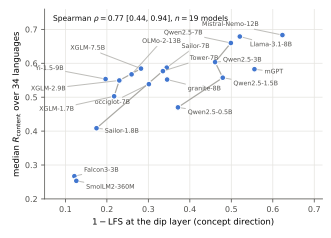
\includegraphics[width=0.62\linewidth]{figs/report/paper_fig2.png}
\caption{Paper Figure 2. The model-level content-transfer result.}\label{fig:g-p2}\end{figure}

\paragraph{Paper Figure 2.} Horizontal axis: $1 - \mathrm{LFS}$ at the dip
layer, the sentence-component share $1-$LFS-VC, so models further right are more
meaning-weighted at their dip. Vertical axis: the model's median
$R_{\mathrm{content}}$ over 34 languages, which is how much a foreign-language
context sentence helps the model predict an English continuation when the
context is the matched translation rather than a mismatched one, normalized by
the English-context benefit. One dot is one of the 19 frozen models; gray
connectors join sizes within a family. What to look for: the cloud rises to
the right, Spearman $0.77$ with model-bootstrap interval $[0.44, 0.94]$;
SmolLM2-360M and Falcon3-3B sit bottom-left, Mistral-Nemo and Llama-3.1-8B
top-right; within a family the connector also rises. Sentence to say: ``Models
whose middle layers weight meaning more make more use of foreign-language
context, and the association holds at the level of whole models, not only
pooled rows.'' Caveat: 19 dots is a small sample; the interval is wide and the
paper says so.

\subsection{The technical report, in order}

\begin{figure}[h]\centering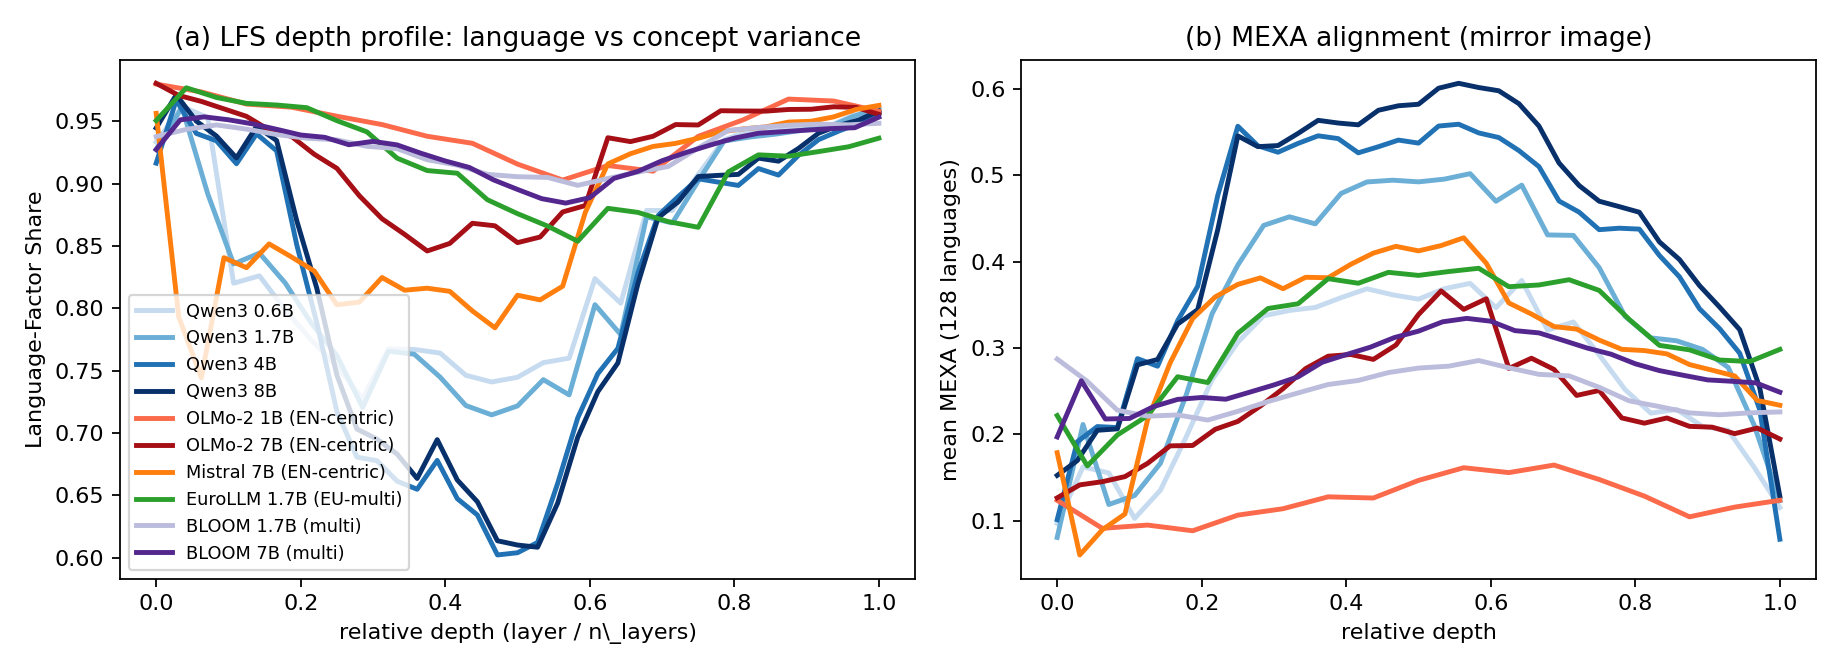
\includegraphics[width=0.95\linewidth]{figs/report/fig1_lfs_depth_profile.png}
\caption{Report Figure 1. (a) LFS by depth, development grid; (b) mean MEXA by depth.}\label{fig:g-r1}\end{figure}

\paragraph{Report Figure 1.} Same axes as paper Figure 1(a), for the ten
development models, coloured by family (Qwen3 blues, OLMo-2 reds, Mistral
orange, EuroLLM green, BLOOM purples). Panel (b) plots mean MEXA, the
published retrieval measure, on the same depth axis. What to look for: (b)
is roughly the mirror image of (a). Where the language share is lowest,
retrieval of the matched translation is easiest. Sentence: ``Two different
instruments agree on where the middle is.'' Do not read (b) as a competition;
it is shown so a reader who knows MEXA can place LFS.

\begin{figure}[h]\centering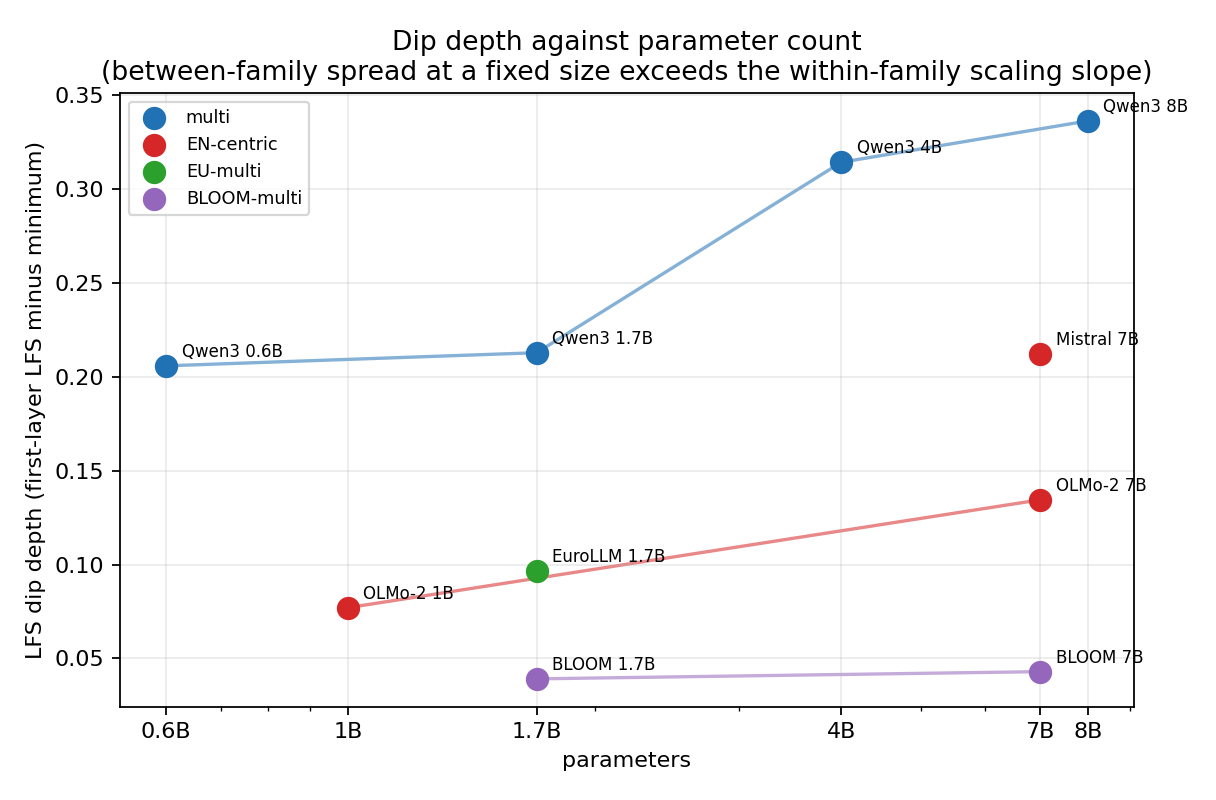
\includegraphics[width=0.66\linewidth]{figs/report/fig7_mix_vs_scale.png}
\caption{Report Figure 2. Dip depth against parameter count.}\label{fig:g-r7}\end{figure}

\paragraph{Report Figure 2 (dip depth against parameters).} Horizontal axis:
parameter count, on a compressed scale. Vertical axis: dip depth. One dot is
one model, coloured by training-mix class; lines join sizes within a family.
What to look for: within a family the line slopes up (scale deepens the dip),
but at a fixed size the vertical spread across families is far larger than
any slope. Near 7B the dots run from BLOOM at $0.04$ through OLMo-2 at $0.13$
and Mistral at $0.21$ to Qwen3-8B at $0.34$. Sentence: ``How a model was
trained moves the dip more than how big it is.'' Caveat: dots within about
$0.02$ of each other, such as Qwen3-1.7B at $0.213$ and Mistral-7B at
$0.212$, are not distinguishable once the bootstrap intervals are attached.

\begin{figure}[h]\centering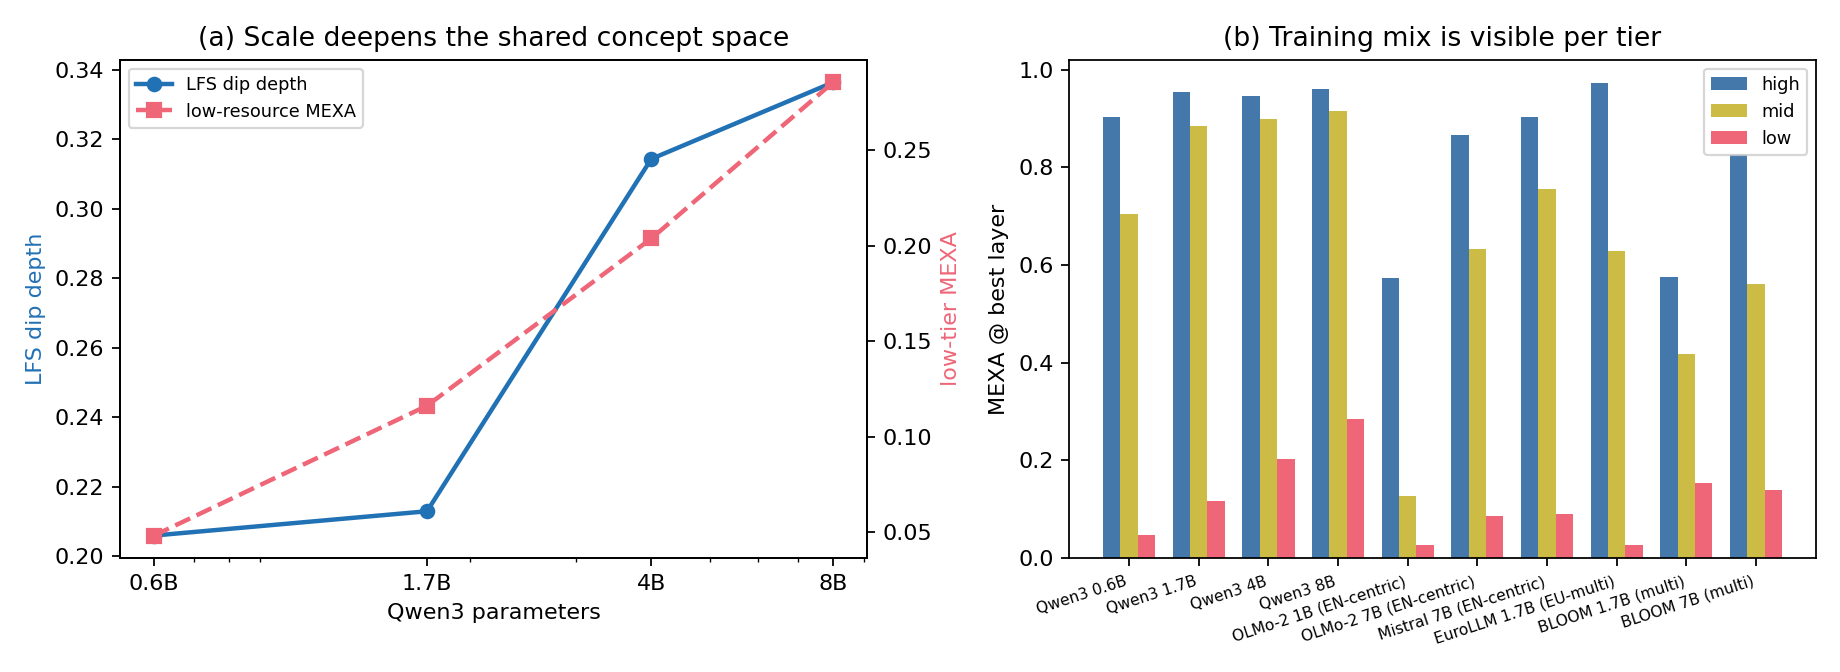
\includegraphics[width=0.95\linewidth]{figs/report/fig2_scaling_tiers.png}
\caption{Report Figure 3. (a) Qwen3 series with two vertical axes; (b) MEXA by resource tier.}\label{fig:g-r2}\end{figure}

\paragraph{Report Figure 3.} Panel (a) has two vertical axes: dip depth on
the left (blue, solid) and low-resource-tier MEXA on the right (red, dashed),
both against Qwen3 size. Read each line against its own axis only; the
crossing point means nothing, because the two scales were chosen
independently. What it shows: both rise with scale within Qwen3. Panel (b):
for each model, three bars, MEXA at the best layer averaged over high-, mid-,
and low-resource languages. What to look for: the low-resource bar is near
the floor for OLMo-2, EuroLLM, and BLOOM, and rises with scale only for
Qwen3. Sentence: ``The training mix is visible tier by tier.'' Caveat: this
is a four-point trend for one family; the paper does not generalize it.

\begin{figure}[h]\centering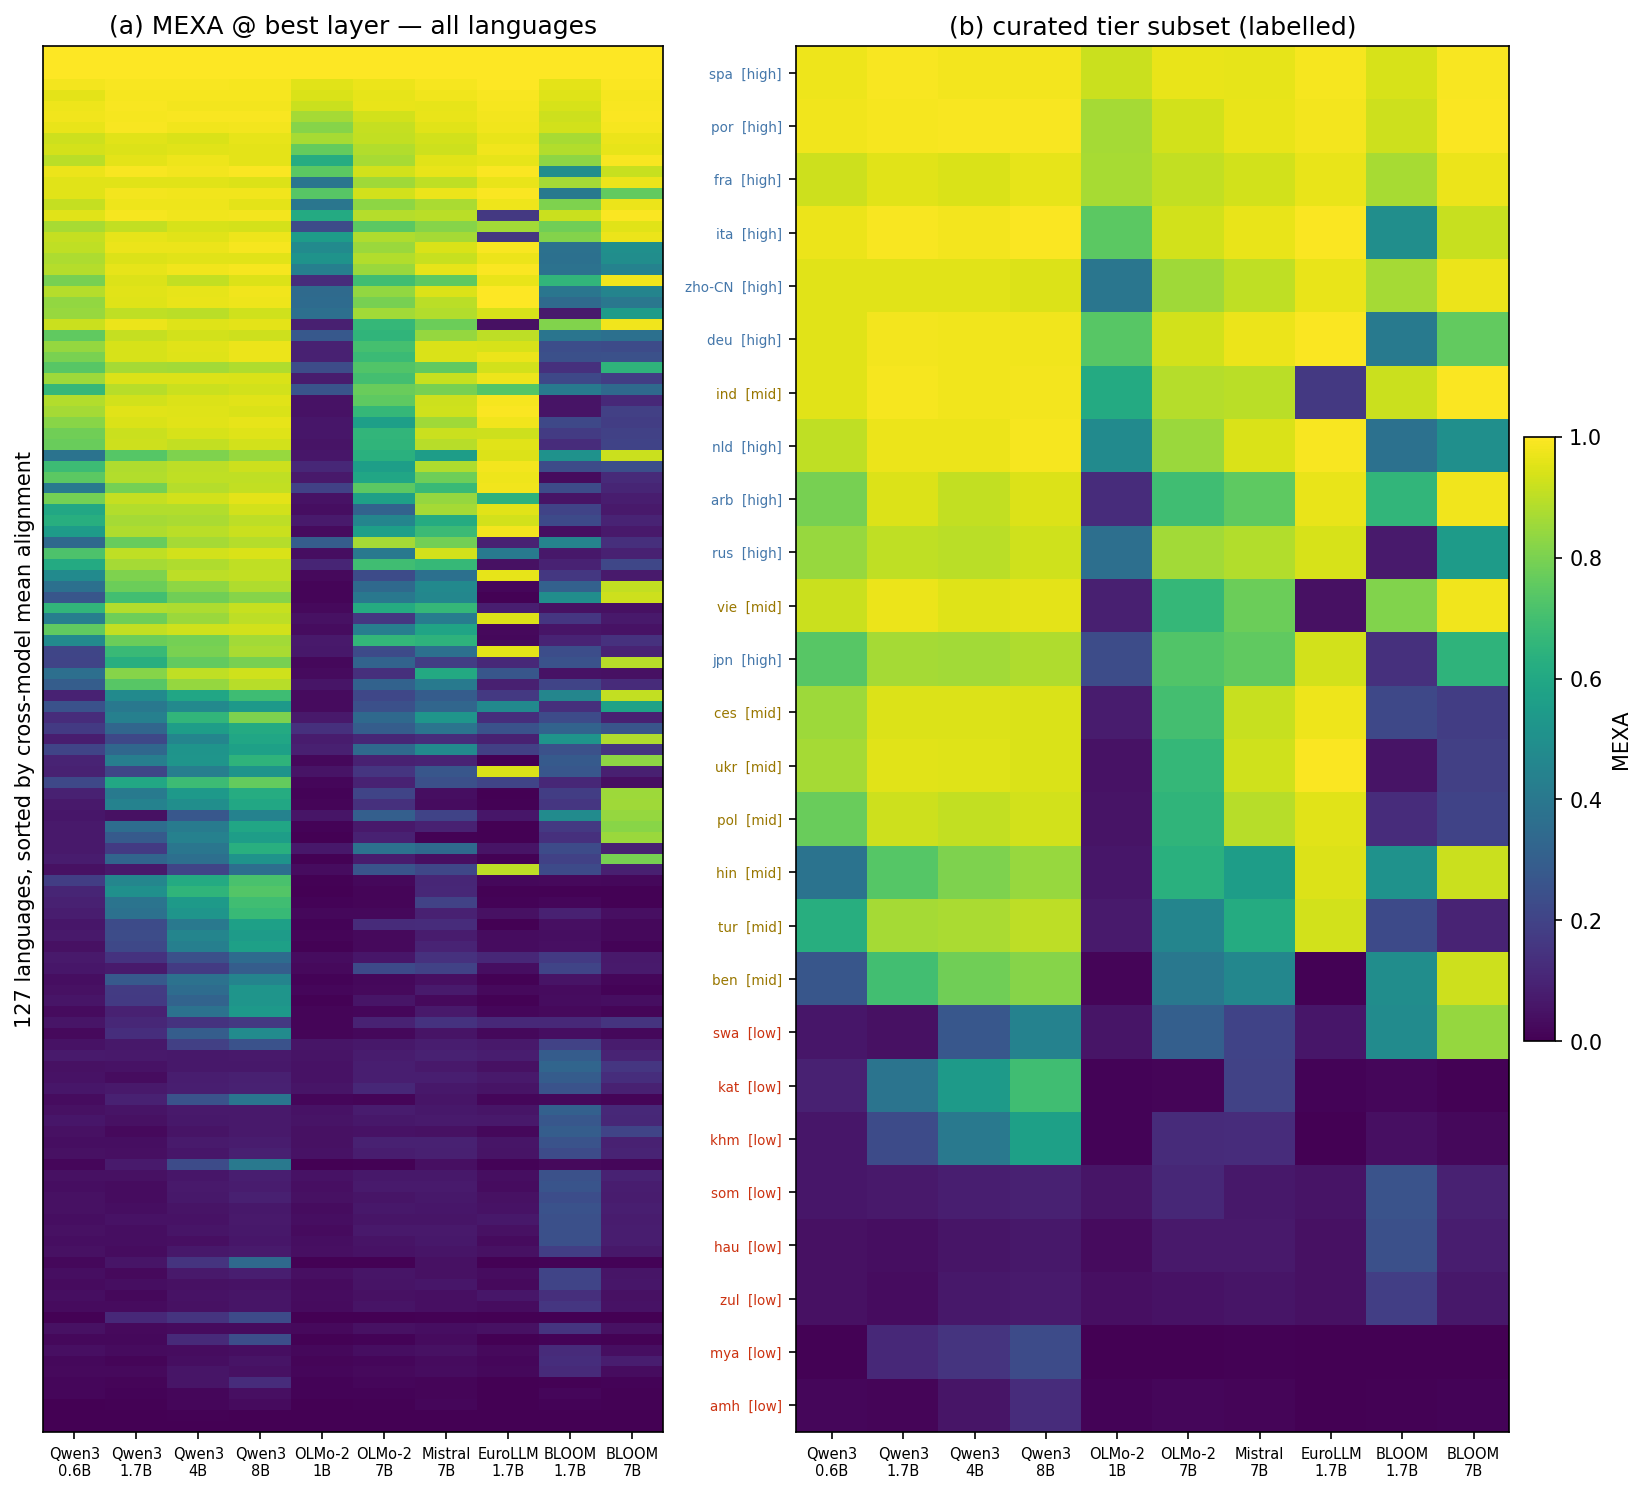
\includegraphics[width=0.95\linewidth]{figs/report/fig6_heatmap.png}
\caption{Report Figure 4. MEXA at the best layer, languages by models.}\label{fig:g-r6}\end{figure}

\paragraph{Report Figure 4 (heatmap).} Rows are 127 languages sorted by their
mean alignment across models; columns are the ten development models; colour
is MEXA at the best layer, dark for 0 and yellow for 1. Panel (b) is a 26
language subset with labels and resource tiers. How to read: run your eye down
a column to see a model's pattern (Qwen3 columns bright far down, OLMo-2
dark outside the top band, EuroLLM bright exactly on its European block);
run across a row to see how a language fares everywhere. The bottom rows are
dark for every model. Sentence: ``The lowest-resource languages are unaligned
in every model; the models differ in how far down the list alignment
reaches.'' This is a reference measure, not an LFS result.

\begin{figure}[h]\centering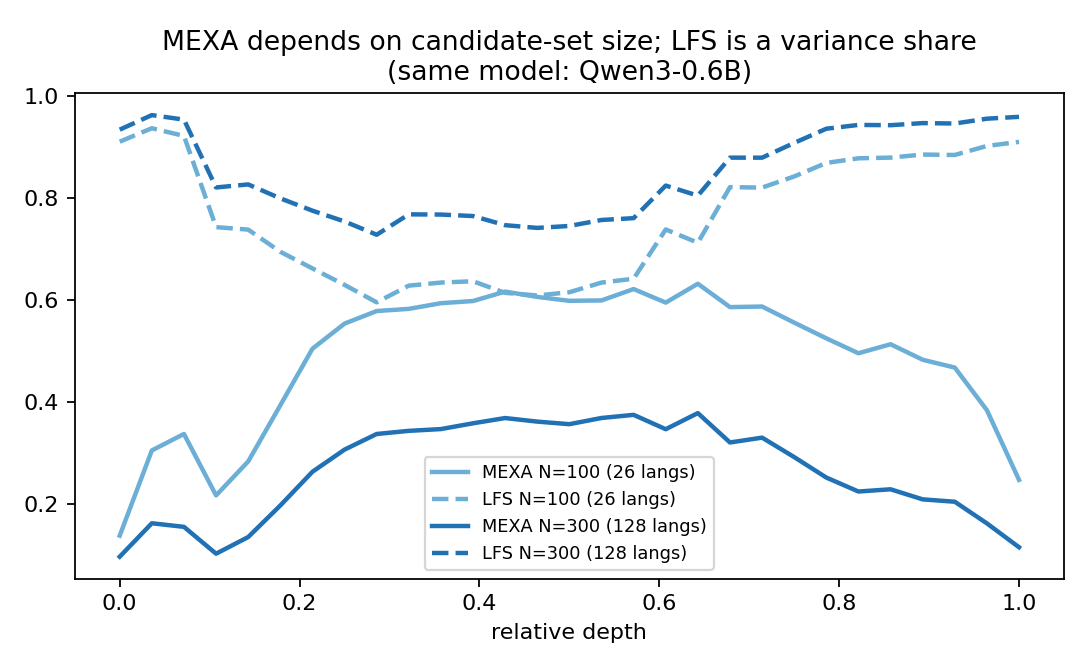
\includegraphics[width=0.7\linewidth]{figs/report/fig5_n_sensitivity.png}
\caption{Report Figure 5. Evaluation-size dependence.}\label{fig:g-r5}\end{figure}

\paragraph{Report Figure 5.} Depth on the horizontal axis; four curves for
one model, Qwen3-0.6B: MEXA (solid) and LFS (dashed) each computed with 100
sentences and 26 languages, and with 300 sentences and 128 languages. What to
look for: the two MEXA curves are far apart (the peak falls from about $0.63$
to $0.38$) because retrieval gets harder with more decoys, while the two LFS
curves nearly coincide. Sentence: ``A retrieval score depends on how many
candidates you gave it; a variance share does not.'' The report quantifies
the small residual dependence of LFS elsewhere rather than claiming exact
invariance.

\begin{figure}[h]\centering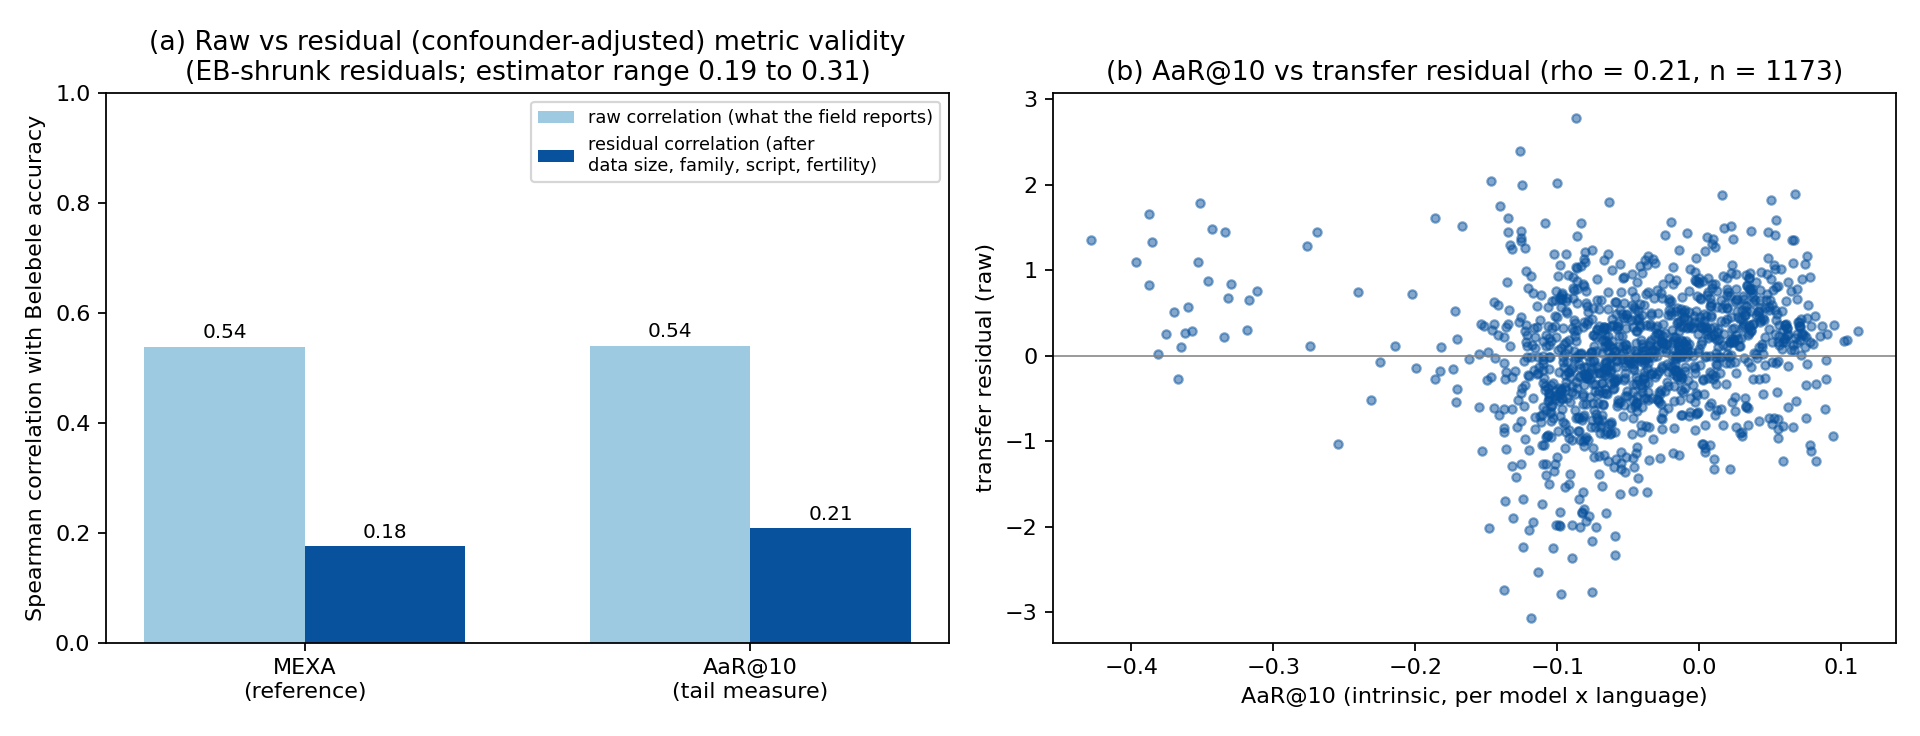
\includegraphics[width=0.95\linewidth]{figs/report/fig8_deflation.png}
\caption{Report Figure 6. Raw and confounder-adjusted validity against benchmark accuracy.}\label{fig:g-r8}\end{figure}

\paragraph{Report Figure 6 (confounder adjustment).} Panel (a): for the tail measure
AaR@10 and, for reference, MEXA, two bars each: the raw Spearman correlation
with Belebele accuracy across (model, language) rows, and the residual
correlation after regressing out training-data size, language family, script,
and tokenizer fertility from both variables. What to look for: both fall from
about $0.5$ to about $0.2$. Panel (b): the residual scatter for AaR@10, 690
rows, a weak positive cloud. Sentence: ``About half of the raw correlation is
data exposure; what survives is the metric's own information.'' The two
measures are not ranked against each other.

\begin{figure}[h]\centering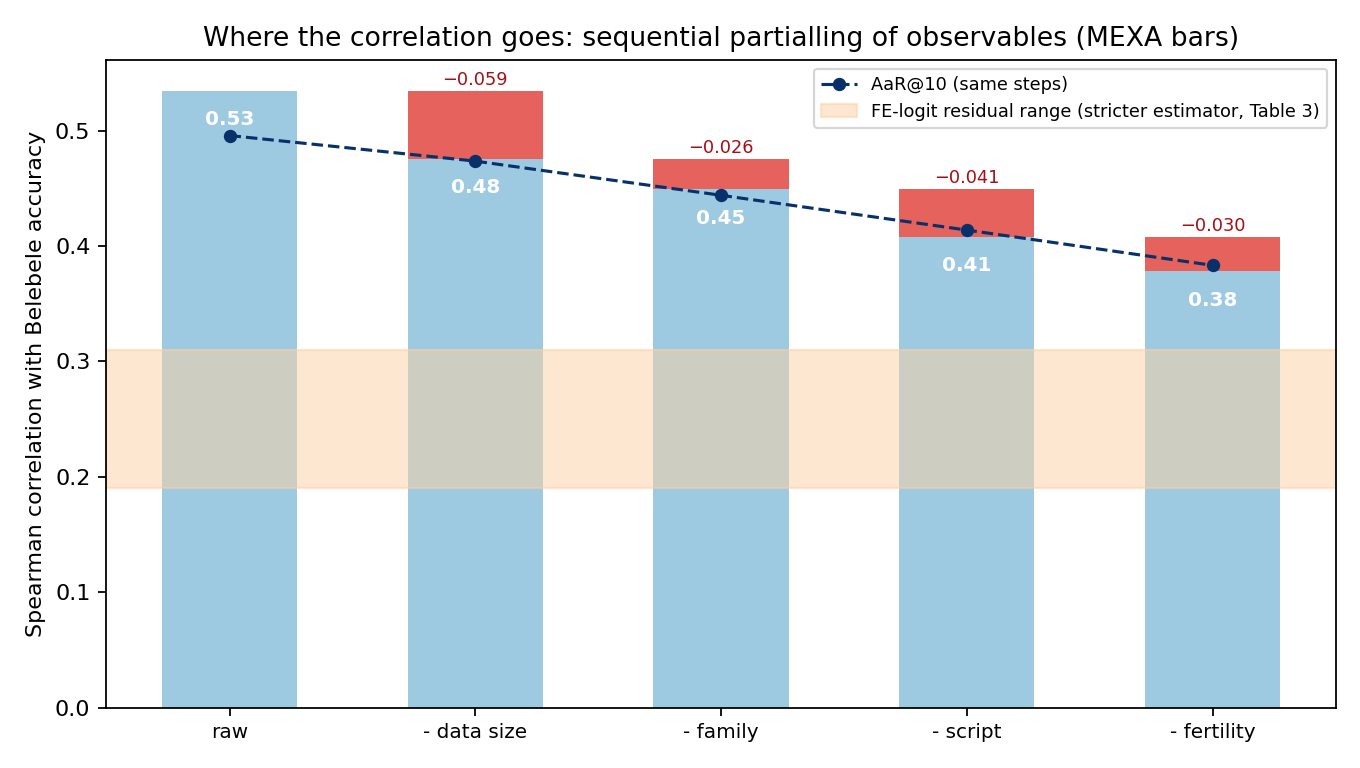
\includegraphics[width=0.78\linewidth]{figs/report/fig11_waterfall.png}
\caption{Report Figure 7. Sequential partialling of observables.}\label{fig:g-r11}\end{figure}

\paragraph{Report Figure 7 (sequential partialling).} Bars from left to right: the raw
correlation, then the correlation after removing data size, then also family,
then also script, then also fertility. The red cap on each bar is the amount
the last control removed. The dashed line repeats the steps for AaR@10. The
shaded band is the stricter fixed-effects estimate of the same quantity,
$0.19$ to $0.31$. What to look for: every control removes some, data size the
most; the sequence stops well above zero. Sentence: ``The correlation is
partly exposure, partly something the metric adds.'' Caveat stated in the
report: the order of controls affects the individual steps, not the endpoint.

\begin{figure}[h]\centering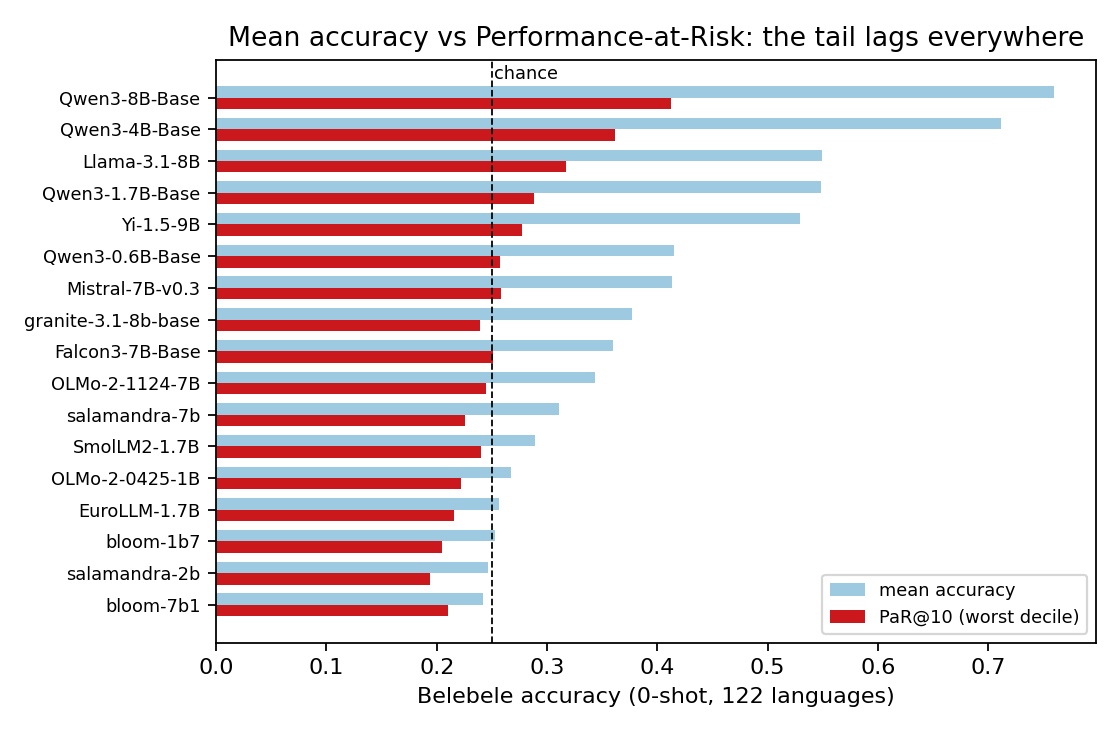
\includegraphics[width=0.7\linewidth]{figs/report/fig9_par.png}
\caption{Report Figure 8. Mean accuracy against worst-decile accuracy.}\label{fig:g-r9}\end{figure}

\paragraph{Report Figure 8 (Performance-at-Risk).} One row per model; light
bar is mean Belebele accuracy across 122 languages, red bar is PaR@10, the
mean accuracy over the worst ten percent of languages. The dashed line is
chance for a four-way benchmark, $0.25$. What to look for: the red bar lags the
light bar for every model, and for several models the red bar sits at chance
while the mean is comfortably above it. Sentence: ``The mean hides languages
on which the model is guessing.''

\begin{figure}[h]\centering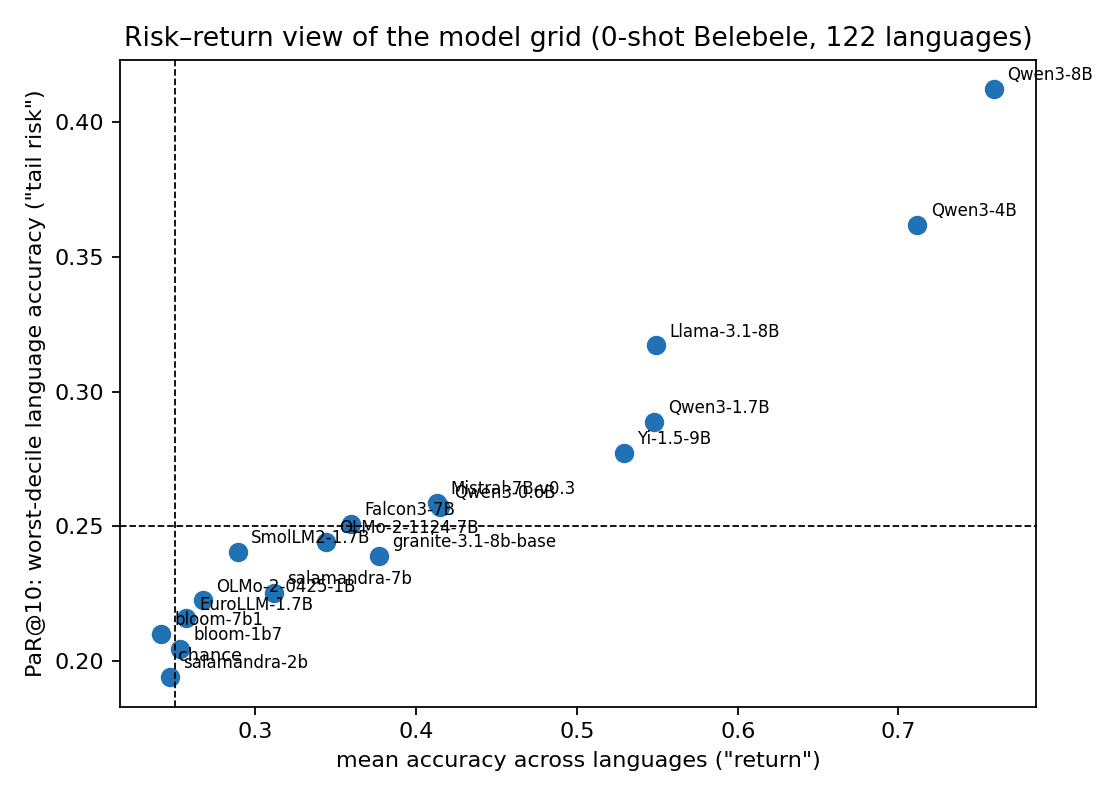
\includegraphics[width=0.66\linewidth]{figs/report/fig13_riskreturn.png}
\caption{Report Figure 9. Mean accuracy against tail accuracy, one dot per model.}\label{fig:g-r13}\end{figure}

\paragraph{Report Figure 9.} The same two numbers as Figure 8, now as a
scatter: mean accuracy horizontally, worst-decile accuracy vertically, dashed
chance lines on both. What to look for: Qwen3-8B is alone in the top right,
a cluster of models sits at the chance corner, and no model is high on one
axis and low on the other. Sentence: ``On this benchmark, serving the tail and
serving the average go together; nobody buys tail robustness by sacrificing
the mean.''

\begin{figure}[h]\centering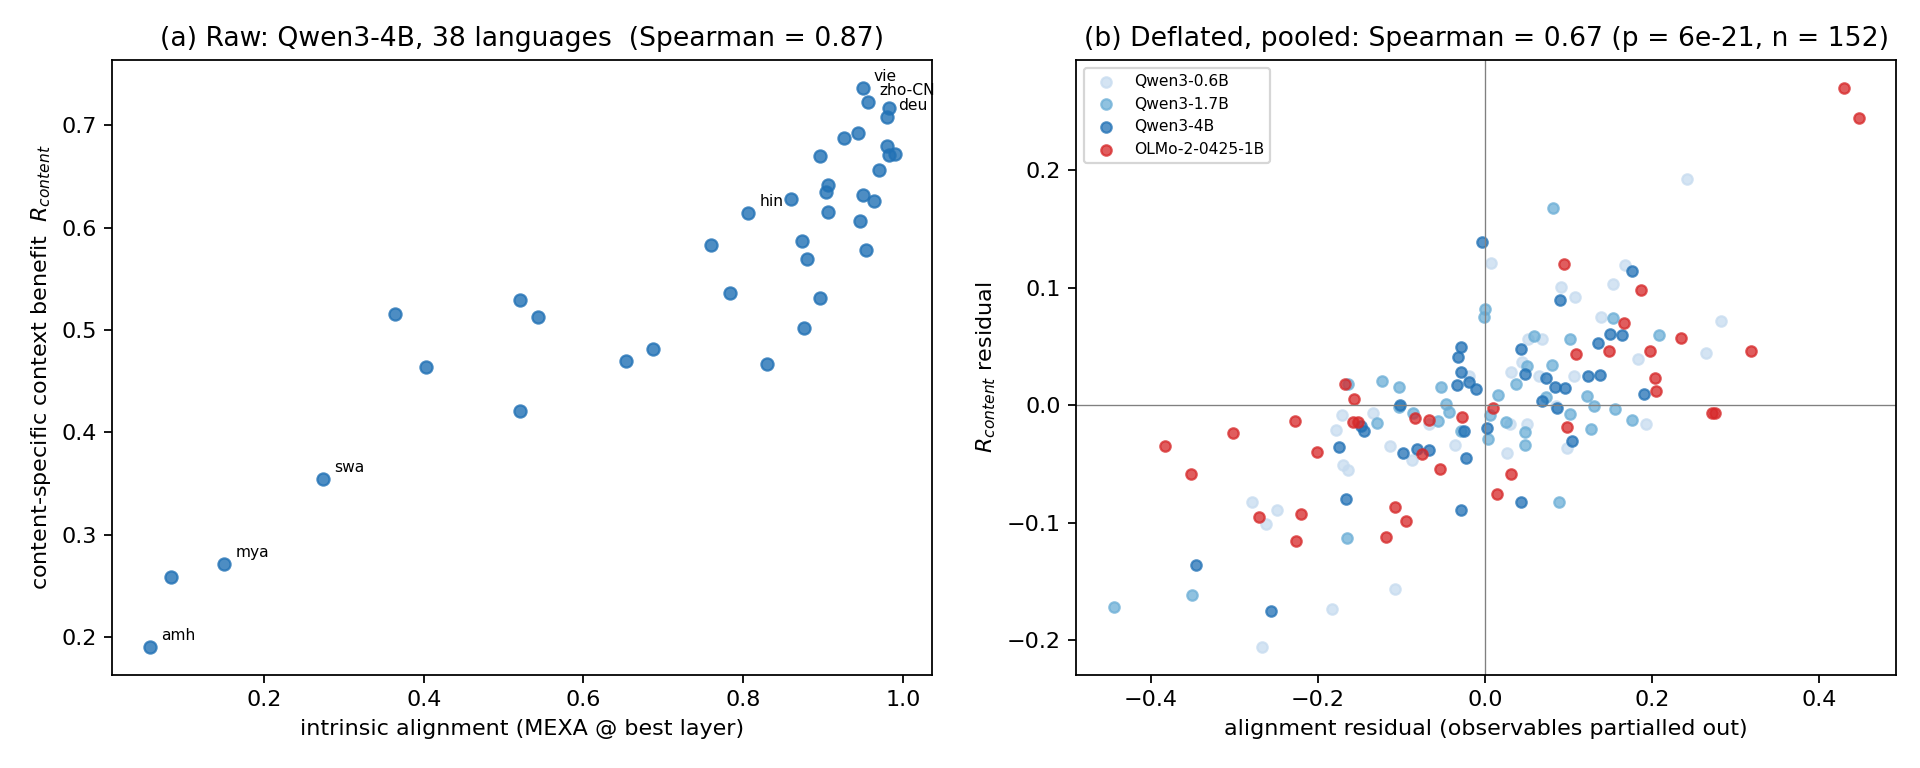
\includegraphics[width=0.95\linewidth]{figs/report/fig10_b2scatter.png}
\caption{Report Figure 10. Alignment against content-specific context benefit.}\label{fig:g-r10}\end{figure}

\paragraph{Report Figure 10.} Panel (a), one model (Qwen3-4B): each dot is a
language, horizontal is its alignment at the best layer, vertical is its
content-specific context benefit $R_{\mathrm{content}}$; Amharic, Burmese,
and Swahili sit bottom-left, German, Chinese, and Vietnamese top-right,
Spearman $0.87$. Panel (b): both axes replaced by their residuals after the
same four controls, pooled over four models and coloured by model; Spearman
$0.67$. What to look for: the cloud in (b) still rises. Sentence: ``The
relation between alignment and context use is not just resource level in
disguise.'' This is the four-model pilot; the 19-model version is paper
Figure 2.

\begin{figure}[h]\centering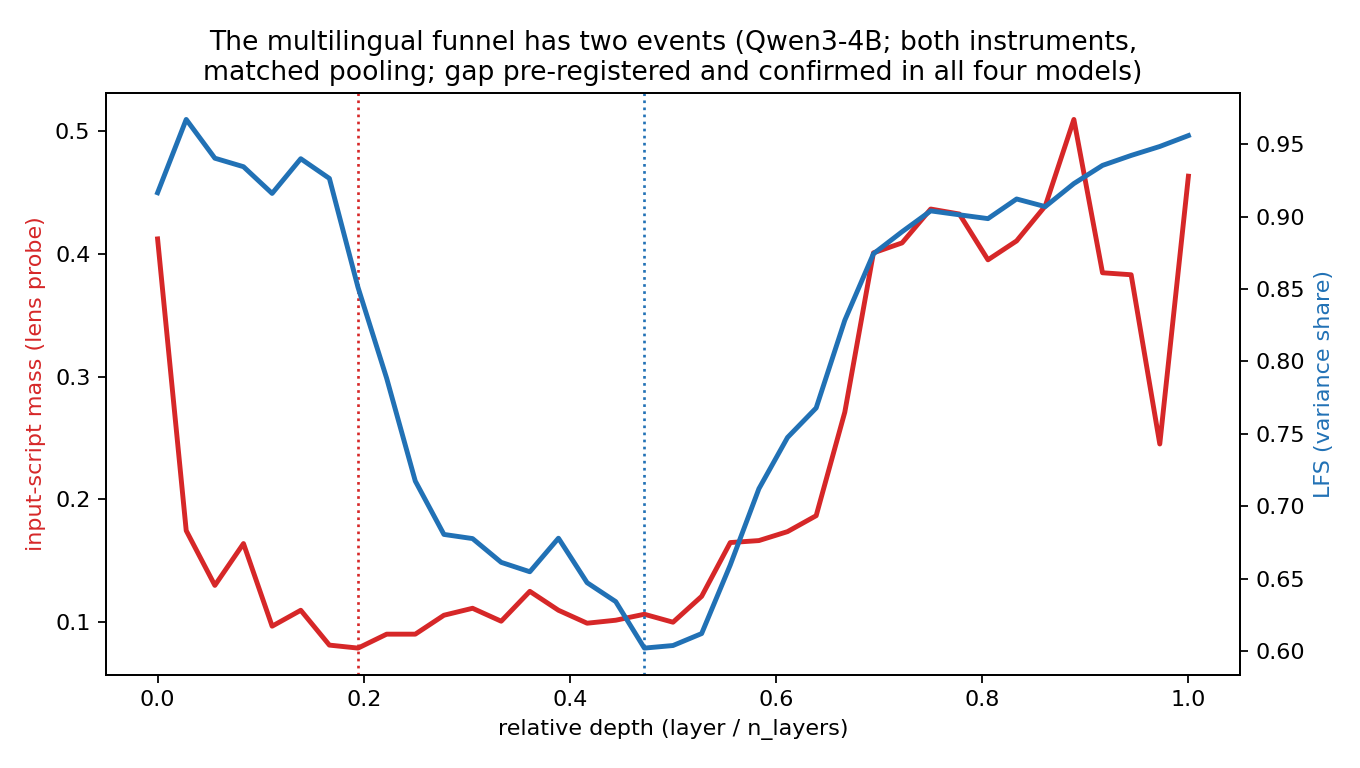
\includegraphics[width=0.78\linewidth]{figs/report/fig12_twoevents.png}
\caption{Report Figure 11. Two instruments on one depth axis.}\label{fig:g-r12}\end{figure}

\paragraph{Report Figure 11 (two events).} Two vertical axes again, so read
each curve against its own. Red, left axis: the share of probability mass the
logit lens puts on tokens in the input's script, which falls steeply by
relative depth $0.2$. Blue, right axis: LFS, which reaches its minimum near
$0.47$. Dotted verticals mark the two minima. Sentence: ``The surface script
is abandoned early; the language share of the variance converges later. They
are two events, not one.'' This is the report's evidence that a logit-lens
measure and a representation measure measure different things.

\begin{figure}[h]\centering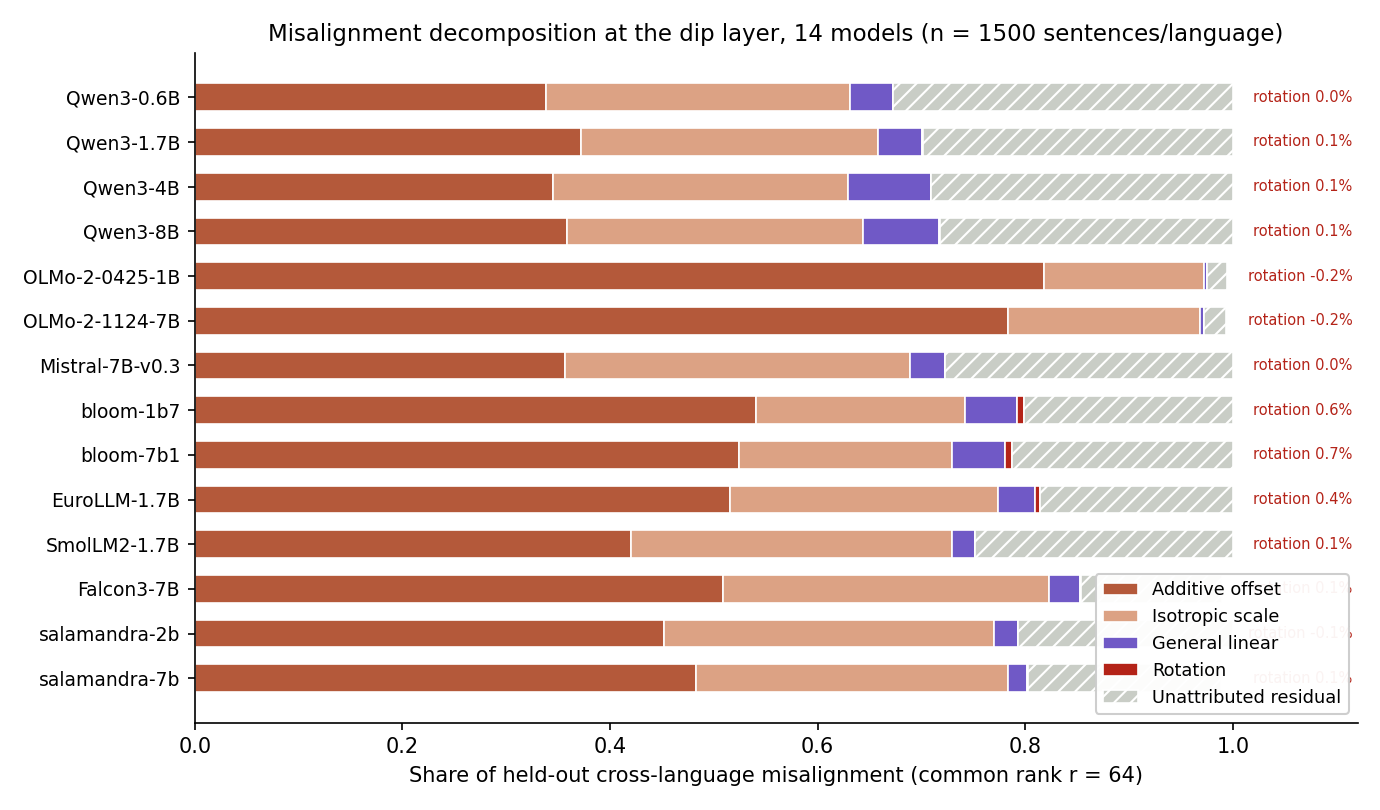
\includegraphics[width=0.95\linewidth]{figs/report/fig15_budget_composition.png}
\caption{Report Figure 12 and paper appendix figure. The misalignment decomposition.}\label{fig:g-r15}\end{figure}

\paragraph{Report Figure 12 (misalignment decomposition).} One stacked bar per
model, at the dip layer, on the 1,500-sentence 1,500-sentence data. The bar is the
held-out cross-language misalignment, split into what a nested sequence of maps
explains: an additive offset (dark), an isotropic scale (light), a general
linear map (purple), a rotation (red, barely visible), and an unattributed
remainder (hatched). Rotation shares are printed at the right. What to look
for: offset plus scale explain $0.63$ to $0.97$ of the misalignment in every
model, rotation never exceeds $0.7$ percent. Sentence: ``Languages differ
mostly by a shift and a stretch, which is exactly what an additive
decomposition can see; the construct boundary of LFS is empirically
harmless here.''

\begin{figure}[h]\centering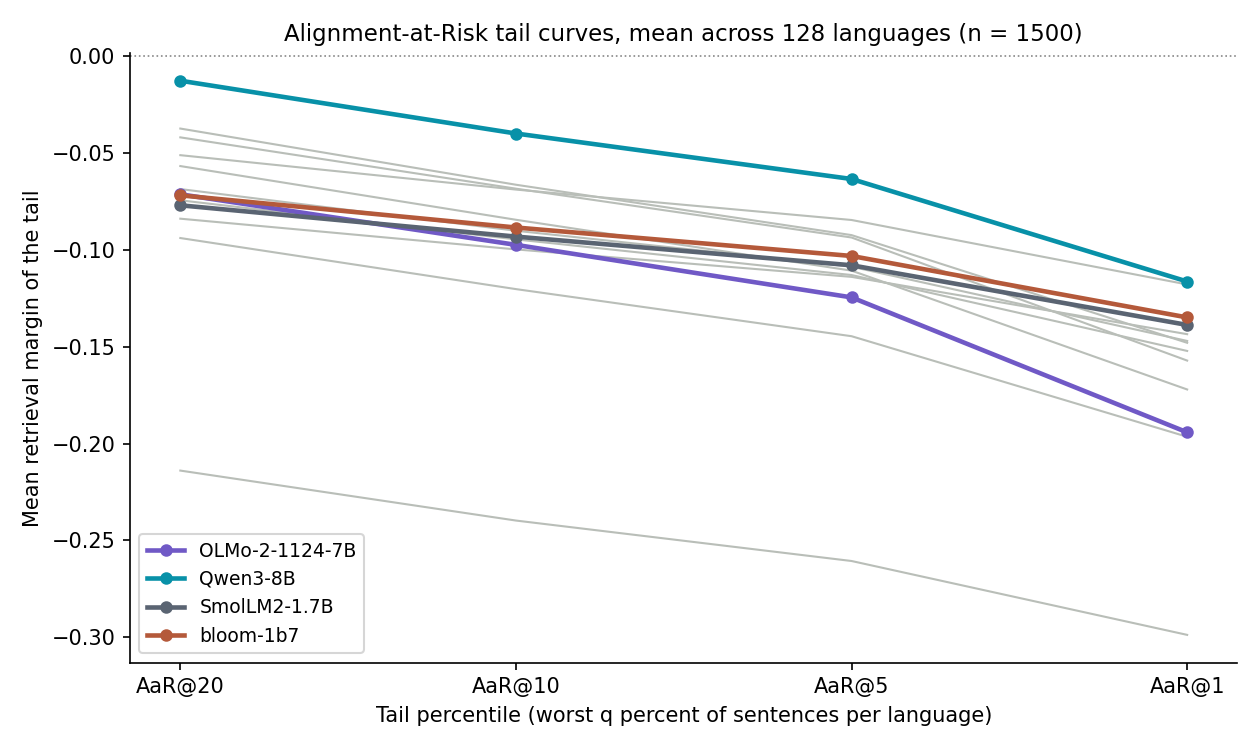
\includegraphics[width=0.78\linewidth]{figs/report/fig16_tail_curves.png}
\caption{Report Figure 13. Alignment-at-Risk tail curves.}\label{fig:g-r16}\end{figure}

\paragraph{Report Figure 13 (tail curves).} Horizontal axis: which tail,
from the worst 20 percent of sentences per language on the left to the worst
1 percent on the right. Vertical axis: the mean retrieval margin of that tail;
negative means the true translation loses to a decoy. Gray lines are 13
models, four highlighted. What to look for: every curve descends to the
right, so the worst sentences fail everywhere; the slope differs. OLMo-2-7B
drops steeply toward the worst 1 percent (rare but severe failures), Qwen3-8B
stays highest, BLOOM and SmolLM2 are flatter and uniformly weak. Sentence:
``Two models with similar means can have different tails; the tail curve
separates catastrophic from broad fragility.''

\begin{figure}[h]\centering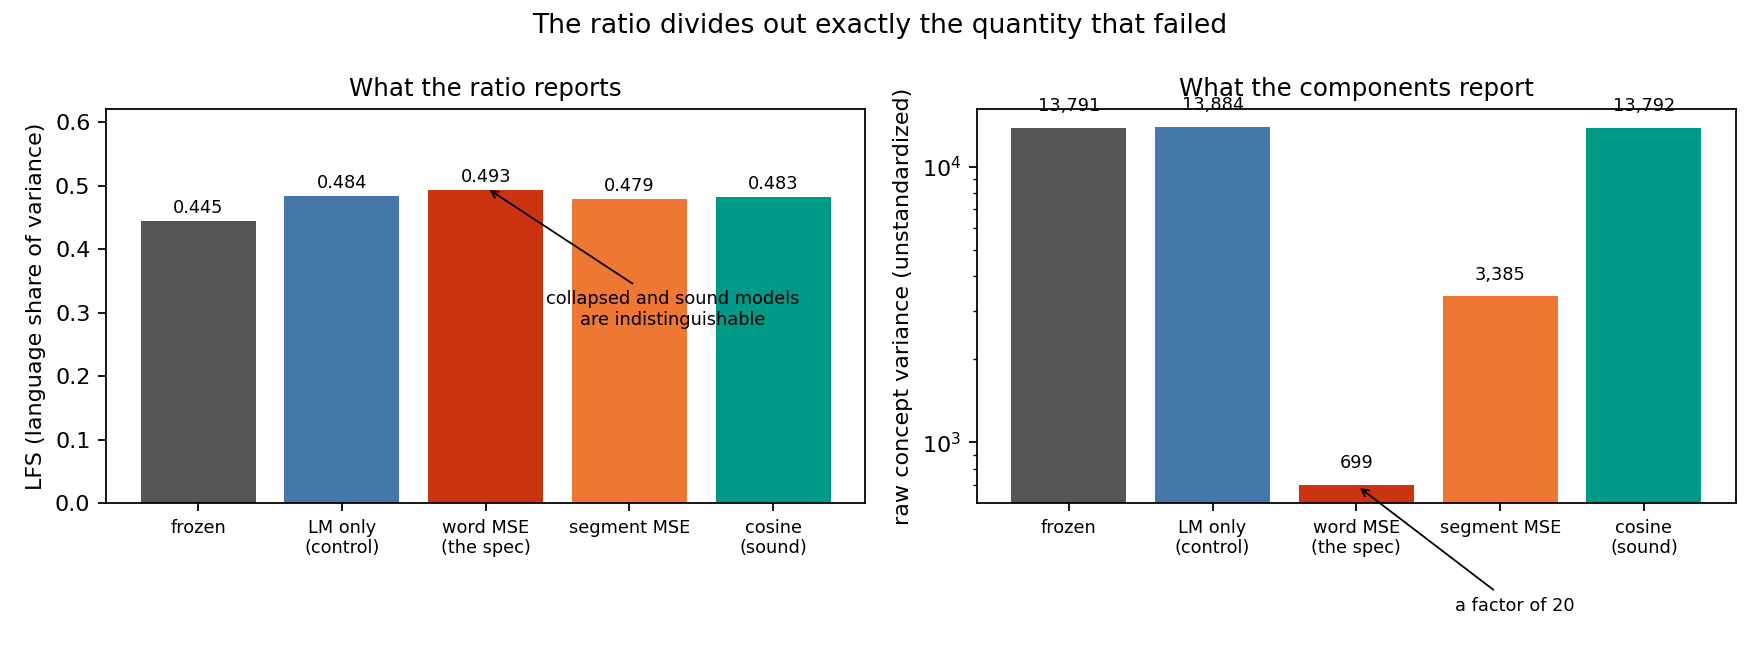
\includegraphics[width=0.95\linewidth]{figs/report/fig17_ratio_hides_scale.png}
\caption{Report Figure 14 and paper appendix figure. The collapse condition read two ways.}\label{fig:g-r17}\end{figure}

\paragraph{Report Figure 14 (ratio against components).} Five training conditions
of Qwen3-0.6B on the word-alignment objectives. Left: LFS for each condition, all
between $0.445$ and $0.493$. Right, logarithmic axis: raw concept variance at
the same layer, $13{,}791$ for the frozen model and $699$ for the word-MSE
condition. What to look for: the condition that lost 95 percent of its concept variance
is indistinguishable from the sound conditions on the left and stands out by a
factor of twenty on the right. Sentence: ``The ratio divides out the quantity
that failed; report the components.'' This is the single most important
figure for the ``why not a score'' argument.

\begin{figure}[h]\centering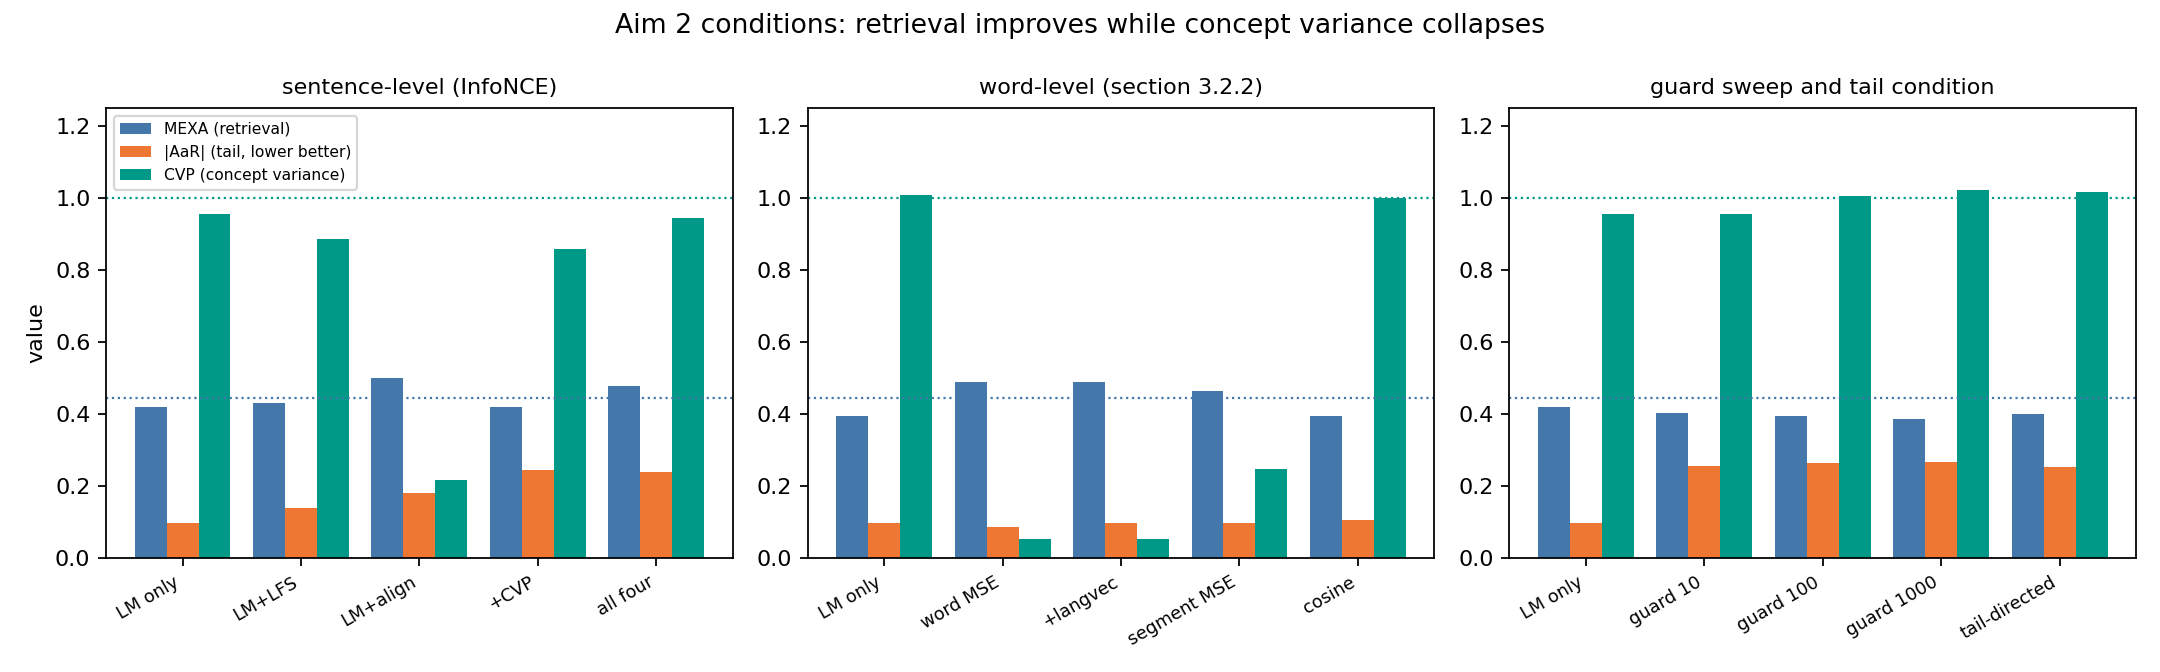
\includegraphics[width=0.95\linewidth]{figs/report/fig18_aim2_arms.png}
\caption{Report Figure 15. Every Aim 2 condition on three instruments.}\label{fig:g-r18}\end{figure}

\paragraph{Report Figure 15 (Aim 2 conditions).} Three panels for three objective
families; within each, one group of three bars per condition: MEXA (retrieval),
the magnitude of AaR (tail, lower is better), and CVP, concept-variance
preservation relative to the frozen model. Dotted lines mark the frozen
model's retrieval and CVP of 1. What to look for: in the word-level panel,
retrieval rises for the word-MSE and language-vector conditions while their CVP
falls to about $0.05$; the cosine condition keeps CVP at 1 and gains nothing.
Sentence: ``Objectives that improve alignment scores can do so by shrinking
the representation; only the preservation measure catches it.''

\begin{figure}[h]\centering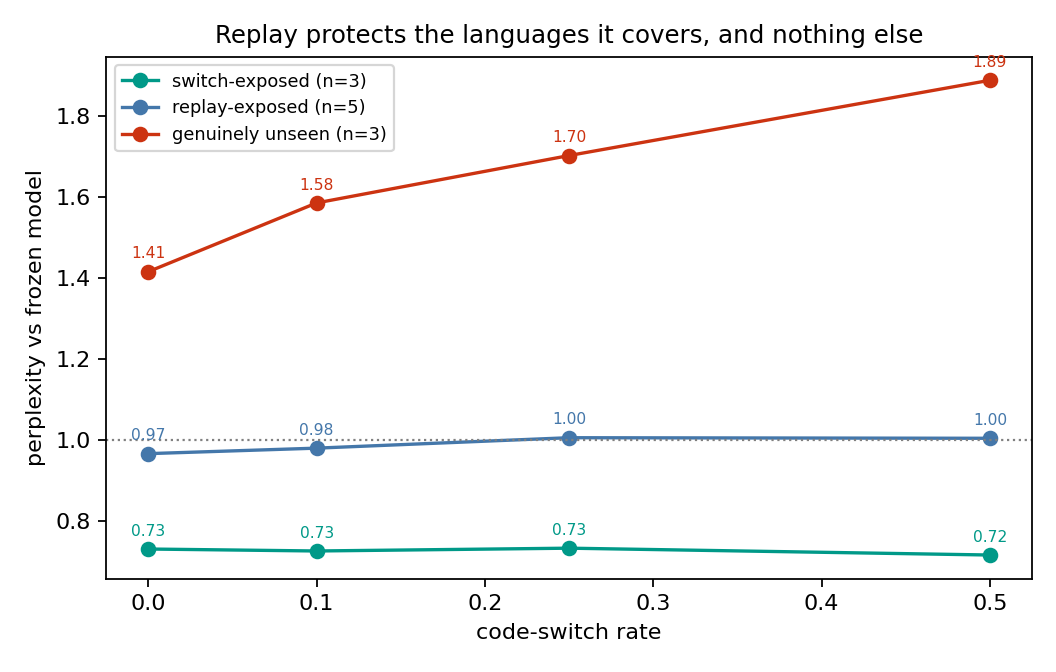
\includegraphics[width=0.66\linewidth]{figs/report/fig20_codeswitch_cost.png}
\caption{Report Figure 16. Code-switched training cost by language group.}\label{fig:g-r20}\end{figure}

\paragraph{Report Figure 16.} Horizontal axis: the code-switch rate used in
training. Vertical axis: perplexity relative to the frozen model, so 1.0 is
unchanged and higher is worse. Three groups of languages: those present in
the switched data, those protected by replay, and those genuinely unseen.
What to look for: the unseen group degrades monotonically, to $1.89$ times
worse at a 50 percent rate, while the other two groups sit at or below 1.
Sentence: ``Replay protects what it contains and nothing else.''

\begin{figure}[h]\centering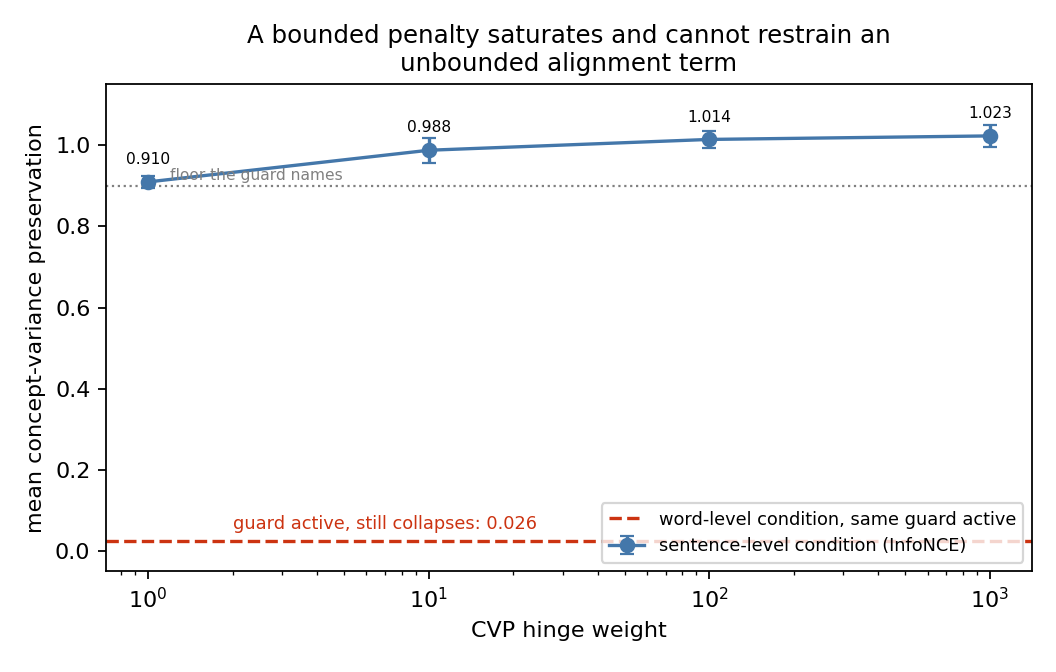
\includegraphics[width=0.66\linewidth]{figs/report/fig21_guard_sweep.png}
\caption{Report Figure 17. The concept-variance guard sweep.}\label{fig:g-r21}\end{figure}

\paragraph{Report Figure 17.} Horizontal axis, logarithmic: the weight on
the concept-variance hinge penalty, from 1 to 1000. Vertical axis: mean
concept-variance preservation. The blue curve is the sentence-level
contrastive condition, rising from $0.91$ to $1.02$ and flattening. The dashed red
line at $0.026$ is the word-level condition with the same guard active. Sentence:
``A bounded penalty saturates; it cannot restrain an unbounded alignment
term, so the guard has to be a constraint, not a weight.''

\begin{figure}[h]\centering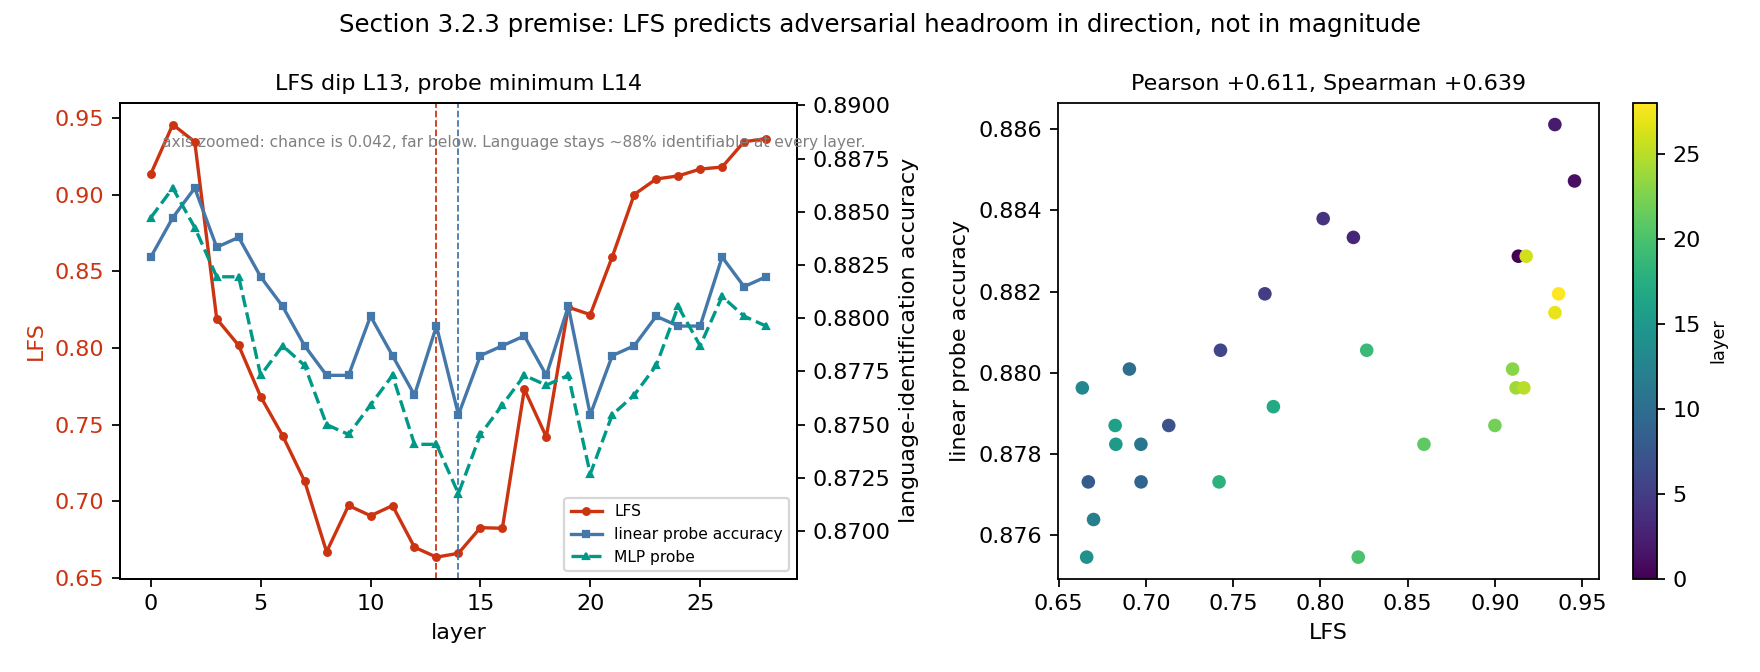
\includegraphics[width=0.95\linewidth]{figs/report/fig19_adversarial_probe.png}
\caption{Report Figure 18. LFS against language-identification probe accuracy.}\label{fig:g-r19}\end{figure}

\paragraph{Report Figure 18 (probe).} Left: layers of Qwen3-0.6B on the
horizontal axis; LFS in red on the left axis; accuracy of a classifier that
predicts the language from the hidden state in blue (linear) and green
(small network) on the right axis. Read the right axis carefully: it runs
from $0.870$ to $0.890$, a zoom; chance is $0.042$. Dashed verticals mark the
LFS minimum at layer 13 and the probe minimum at layer 14. Right: the same
29 layers as a scatter, LFS against probe accuracy, Pearson $0.61$. What to
look for: the curves move together in direction, but the probe never drops
below 87 percent. Sentence: ``Even at the dip, the language is almost
perfectly readable from the representation; the dip is about the share of
variance, not about erasing language identity.'' This is why ``lower LFS''
must never be read as ``language-agnostic''.

\subsection{Figure-measure habits worth keeping}

\begin{itemize}[leftmargin=1.2em]
\item Find the null or the chance line before judging any level. LFS has
$0.298$ on this grid; the benchmark has $0.25$.
\item A depth axis is relative unless it says ``layer''; the same relative
depth is a different layer in a 25-layer and a 49-layer model.
\item Two vertical axes (report Figures 3a and 11) invite a false measure of
the crossing point. Read each curve against its own axis.
\item A ratio next to a raw component (report Figure 14) is the habit the
paper asks the field to adopt.
\item Every number in a figure traces to an artifact in the claims ledger;
if a reviewer asks where a bar came from, the answer is a file path and a job
identifier.
\end{itemize}

\clearpage
\section{Study plan, checklist, and reading list}
\label{ch:plan}

\subsection{The four-hour version}

Three hours forty-five minutes for the day before the Koehn meeting, assuming
linear algebra from coursework and no transformers or analysis of variance.
Chapter~\ref{ch:lfs} precedes the statistics on purpose.

\begin{description}[leftmargin=3.2cm, style=nextline, itemsep=3pt]
\item[0:00 to 0:15, vectors] Chapter~\ref{ch:ml}, why a hidden state is a vector. Exercise: cosine similarity and a first look at anisotropy.
\item[0:15 to 0:50, the model] Chapter~\ref{ch:llm}: tokenization and fertility, embeddings and the residual stream, attention read once. Figure~\ref{fig:block}. Three facts: layer $0$ is the embedding output, every layer shares one $D$-dimensional space, pooling is part of the measurement.
\item[0:50 to 1:05, translation data] Chapter~\ref{ch:mt}: parallel data, translationese, the MEXA paragraph. Figure~\ref{fig:g-r6}, rows read as resource tiers.
\item[1:05 to 1:55, LFS] Chapter~\ref{ch:lfs} in full. Rederive the whiteboard table until $1.5/17.5 = 0.086$ comes unaided; type the exercise ``LFS from scratch'' and check its three printed lines. Figure~\ref{fig:grid}.
\item[1:55 to 2:30, statistics] Chapter~\ref{ch:stats}: the decomposition and bootstrap subsections. Exercise: verify the decomposition and the null by simulation. Then Figure~\ref{fig:bootstrap}: say why models, not rows, are the unit.
\item[2:30 to 3:00, results] Chapter~\ref{ch:figures}, the two paper figures. Figure~\ref{fig:g-p1}: axes, one line, the null line at $0.298$. Then Figure~\ref{fig:g-p2} and the ten numbers in \texttt{docs/KOEHN\_MEETING\_BRIEF\_2026-09-05.md}.
\item[3:00 to 3:20, limits] Chapter~\ref{ch:lfs}: the boundary subsection and what LFS relates to. Figure~\ref{fig:collapse_trained}. Then the MEXA, pooling, and ANOVA answers in Chapter~\ref{ch:defense}.
\item[3:20 to 3:30, aloud] The ten-second, thirty-second, and two-minute versions, then the whiteboard example cold, standing.
\item[3:30 to 3:45, self-test] The ten questions below, answers written first.
\end{description}

\textbf{Skipped relative to the eight-hour plan, and why that is safe.}
\begin{itemize}[itemsep=1pt]
\item Chapter~\ref{ch:ml} regression, gradient descent, softmax, XOR, PCA: LFS trains nothing; in the meeting least squares is the one phrase ``after controlling for exposure, family, script, and fertility''.
\item Chapter~\ref{ch:llm} attention exercise, MLP, normalization, training loop, logit lens: LFS reads the residual stream and never generates; Koehn's recorded questions concern pooling and the shape.
\item Chapter~\ref{ch:mt} alignment history, the ``think in English'' list, the Aim~2 options: the brief scripts the one answer that needs them.
\item Chapter~\ref{ch:stats} residualization and cluster-bootstrap exercises, REML, multiple comparisons: read the figures; the intervals are already computed.
\item The eighteen report figures and the misalignment decomposition: the meeting opens on paper Figure~1 and stays there.
\item The full question bank: the self-test replaces it; return to the bank if time remains.
\end{itemize}

\textbf{Self-test, fifteen minutes.}
\begin{enumerate}[itemsep=1pt]
\item LFS and its parts? $\SSl/(\SSl+\SSc)$: weighted spread of language means over that plus the sentence-mean spread; residual reported, not included.
\item The whiteboard value? $1.5/17.5 = 0.086$; languages differ by a constant offset, sentences by far more.
\item Why standardize jointly? Per-language standardizing subtracts the language means being measured.
\item Pure-noise value here? $(L-1)/(L+N-2) = 0.298$ at 128 by 300; compare only at a fixed grid.
\item Layer $0$, and why layers compare? Embedding output; the residual stream is a running sum, so all layers share one space.
\item Dip depth range, tracking what? $0.039$ (BLOOM-1.7B) to $0.336$ (Qwen3-8B); recipe more than size.
\item The behavioral result, with unit? Spearman $0.508$, model bootstrap $[0.19, 0.71]$, 19 models, 13 families, after controls.
\item What LFS cannot see? Uniform shrinkage: norm 451 to 42, concept variance 13{,}791 to 699, LFS $0.445$ to $0.493$; hence raw components beside the ratio.
\item MEXA in one line? Is the English translation a sentence's nearest neighbour among $N$ candidates; a published reference measure for a different question.
\item Why resample models, not rows? Rows within a model are correlated and the claim is about models.
\end{enumerate}

\subsection{Three weeks to the paper, then the long arc}

\begin{description}[leftmargin=2.9cm, style=nextline, itemsep=3pt]
\item[Days 1 to 3: own the instrument] Chapter~\ref{ch:lfs}. Rederive the worked example and the null by hand; type the \texttt{lfs} exercise; open \texttt{results/grid/Qwen3-8B-Base/metrics.json} and explain the profile layer by layer. Read \texttt{reports/lfs\_math.pdf} and the paper draft Sections 3 and 5.
\item[Days 3 to 6: the transformer] Chapter~\ref{ch:llm} and Chapter~\ref{ch:ml} Sections 1.4 to 1.7. Do the attention and XOR exercises. Read Jurafsky and Martin's transformer and LLM chapters; skim Vaswani et al.\ (2017); read the residual-stream section of Elhage et al.\ (2021); read nostalgebraist's logit-lens post and Timkey and van Schijndel (2021).
\item[Days 6 to 10: statistics] Chapter~\ref{ch:stats}. Do the decomposition, null, residualization, and cluster-bootstrap exercises. Read one ANOVA chapter (any introductory text), Efron and Tibshirani chapters 6 and 7, and Gelman and Hill on fixed effects and clustered data.
\item[Days 8 to 14: Koehn's literature] Chapter~\ref{ch:mt}. Read Koehn (2020) on the transformer, multilingual models, and evaluation; Federmann et al.\ (2022) NTREX; Conneau et al.\ (2018); Marchisio et al.\ (2020 to 2022); Kargaran et al.\ (2025) MEXA in full; Bandarkar et al.\ (2024) Belebele; Ahia et al.\ (2023); Briakou et al.\ (2023).
\item[Days 10 to 16: the debate] Wendler et al.\ (2024); Shani and Basirat (2025); Tezuka and Inoue (2025); Zhao et al.\ (2024); Bafna et al.\ (2025); Dumas et al.\ (2025); Kornblith et al.\ (2019); Chang, Tu, and Bergen (2022). For each, one sentence on its claim and one on what LFS adds or contradicts.
\item[Ongoing: foundations] Chapter~\ref{ch:ml} in full; Goodfellow, Bengio, and Courville chapters 2, 5, 6, 8, 10; Murphy's \emph{Probabilistic Machine Learning: An Introduction} on linear models and inference; a linear algebra refresher (Strang, or the \emph{Deep Learning} book chapter 2).
\end{description}

\subsection{Practice}

Say the ten-second, thirty-second, and two-minute versions aloud once a day.
Once a week, have someone read Chapter~\ref{ch:defense} questions in random
order. Before the Koehn meeting, redo the whiteboard example cold. Every
number you say should be one you can point to in the assessment document or
the claims ledger.

\subsection{The concept checklist}

Tick each when you can explain it to a first-year student in two minutes
without notes. Items marked $\star$ are the must-know set for defending
LFS; the rest are what makes you credible and lets you answer the follow-up.

\paragraph{Why learn at all.}
$\star$ rules versus examples; $\star$ parameters, loss, optimization;
$\star$ supervised, unsupervised, self-supervised, reinforcement;
$\star$ where pretraining, post-training, and measurement sit.

\paragraph{Machine learning basics.}
model, parameters, loss; $\star$ vectors, dot product, norm, cosine; matrix
as many dot products; $\star$ linear regression, least squares, residuals,
$R^2$; $\star$ ridge; gradient, gradient descent, learning rate, batches,
Adam; sigmoid, softmax, logits, cross-entropy, negative log-likelihood,
perplexity; $\star$ train/validation/test, overfitting; regularization,
early stopping, cross-validation; MLP, nonlinearity, backpropagation,
autograd; embeddings; PCA, SVD, eigenvalues, effective rank, participation
ratio; epochs, seeds, checkpoints, pretraining, fine-tuning, inference.

\paragraph{Language models.}
$\star$ next-token prediction; $\star$ tokenization, BPE, vocabulary,
fertility; embedding matrix; positional information (rotary); $\star$
residual stream; $\star$ hidden state per layer, layer 0; attention (query,
key, value, scores, causal mask, heads); MLP block; LayerNorm/RMSNorm,
pre-norm; $\star$ massive activations, anisotropy; unembedding, logits, tied
embeddings; teacher forcing; perplexity; training loop, Adam, schedules;
$\star$ base versus instruct, SFT, RLHF/DPO; greedy versus sampling,
temperature; $\star$ fp16/bf16/fp32; $\star$ mean versus last-token pooling;
$\star$ logit lens and its validity limit; linear probes; activation
patching; CKA; scaling versus recipe.

\paragraph{Machine translation and multilingual NLP.}
SMT versus NMT versus LLM; $\star$ parallel and n-way parallel corpora;
sentence alignment; $\star$ NTREX, FLORES, WMT; documents and purged splits;
$\star$ translationese and direction; BLEU, chrF, COMET; contamination;
chance floors; $\star$ resource tiers, families, scripts; curse of
multilinguality; cross-lingual transfer; incidental bilingualism; tokenizer
fairness; cross-lingual word-embedding alignment, Procrustes, MUSE, hubness,
CSLS; sentence embeddings, LASER/LaBSE; $\star$ MEXA, AaR, Information
Parity; $\star$ the ``think in English'' debate and its papers; Aim 2
methods (parallel data, code-switching, alignment losses, adversarial,
preference); Belebele, INCLUDE, Global-MMLU, MGSM.

\paragraph{Statistics of measurement.}
$\star$ variance and sums of squares; $\star$ one-way and two-way ANOVA;
$\star$ balance and orthogonality; $\star$ degrees of freedom; mean squares;
expected mean squares; variance components; REML; $\star$ standardization
and invariances; $\star$ Pearson versus Spearman; $\star$ confounding;
$\star$ residualization; $\star$ fixed effects; logit transform above a
floor; cluster-robust errors; $\star$ bootstrap; $\star$ cluster and crossed
bootstrap; $\star$ unit of generalization; effective sample size;
leave-one-out; Benjamini--Hochberg; $\star$ preregistration; minimum
detectable effect; construct and predictive validity; reliability,
ceilings, Spearman--Brown; $\star$ Goodhart's law.

\paragraph{Linear algebra and interpretability tools.}
projection; orthogonal matrices and rotations; Procrustes; PCA/SVD;
whitening; effective rank; Gini; ridge regression; linear probes; activation
patching; CKA; logit lens.

\paragraph{LFS itself.}
balanced grid; fp32 mean pooling; joint z-scoring; grand, language, sentence
means; $\SSl$, $\SSc$, $\SSr$ and the multipliers; the ratio; the residual's
role; the decomposition proof; boundedness; scale invariance; rotation
invariance; the null and its three consequences; near size-independence; dip
depth, interior minimum, endpoint recovery; values above 0.5; additive
boundary and the misalignment decomposition; variance share versus separability;
collapse blind spot and the profile fix; content transfer versus benchmarks;
observation versus intervention; the family and the no-averaging rule; MEXA
as a different question.

\subsection{Reading list with what to take from each}

\begin{description}[leftmargin=0pt, style=nextline, itemsep=2pt]
\item[Jurafsky and Martin, \emph{Speech and Language Processing}, 3rd ed.\ draft (free online)] transformers, LLMs, MT chapters: the vocabulary and the standard pictures.
\item[Koehn, \emph{Neural Machine Translation} (2020)] the transformer from an MT perspective, multilingual models, evaluation. Read for framing as much as content.
\item[Koehn, \emph{Statistical Machine Translation} (2010)] chapters on parallel data and evaluation; skim for history.
\item[Goodfellow, Bengio, Courville, \emph{Deep Learning} (free online)] ch.\ 2 linear algebra, 5 ML basics, 6 MLPs, 8 optimization, 10 sequence models.
\item[Murphy, \emph{Probabilistic Machine Learning: An Introduction} (free online)] linear models, logistic regression, inference basics.
\item[Efron and Tibshirani, \emph{An Introduction to the Bootstrap}] chapters 6 and 7; then any short note on cluster bootstrap.
\item[Gelman and Hill, \emph{Data Analysis Using Regression and Multilevel/Hierarchical Models}] fixed effects, clustered data, why the unit matters.
\item[Searle, Casella, McCulloch, \emph{Variance Components}] the balanced two-way chapter, for REML.
\item[Vaswani et al.\ 2017] attention is all you need. Read Sections 3 and 4.
\item[Elhage et al.\ 2021, \emph{A Mathematical Framework for Transformer Circuits}] the residual-stream section only.
\item[nostalgebraist 2020] the logit lens post; then Wendler et al.\ 2024.
\item[Timkey and van Schijndel 2021; Sun et al.\ 2024] rogue dimensions and massive activations.
\item[Kargaran et al.\ 2025 (MEXA)] read fully; know the exact scoring rule and the reported correlations.
\item[Conneau et al.\ 2018; Artetxe et al.\ 2018; Marchisio et al.\ 2020--2022] cross-lingual embedding alignment and Koehn's group's contributions.
\item[Shani and Basirat 2025; Tezuka and Inoue 2025; Zhao et al.\ 2024; Bafna et al.\ 2025; Dumas et al.\ 2025] the layerwise-sharing debate.
\item[Kornblith et al.\ 2019 (CKA); Chang, Tu, Bergen 2022] representational similarity and multilingual geometry.
\item[Federmann et al.\ 2022 (NTREX); Bandarkar et al.\ 2024 (Belebele); Romanou et al.\ 2025 (INCLUDE)] the datasets.
\item[Ahia et al.\ 2023; Petrov et al.\ 2023] tokenizer fertility and fairness.
\item[Briakou, Cherry, Foster 2023] incidental bilingualism drives translation ability.
\item[Nosek et al.\ 2018; Strathern 1997] preregistration; Goodhart's law.
\end{description}

\subsection{Project documents to know by location}

\begin{description}[leftmargin=0pt, style=nextline, itemsep=1pt]
\item[\texttt{docs/AIM1\_ASSESSMENT\_FOR\_ICLR\_2026-09-04.md}] sub-aim verdicts, every number with its artifact.
\item[\texttt{paper/iclr2027/main.tex}, \texttt{claims\_ledger.csv}] the paper and the map from numbers to artifacts and jobs.
\item[\texttt{docs/AIM1\_NEXT\_EXPERIMENTS\_2026-09-05.md}] the candidate experiments, costs, and frozen predictions.
\item[\texttt{code/pilot\_metrics.py}] the canonical estimator.
\item[\texttt{docs/DISCREPANCY\_LEDGER.md}] every correction, with mechanism. Reviewers reward it when you volunteer it.
\item[\texttt{proposal/NSF\_Proposal\_on\_Multilingual\_LLMs.pdf}] Section 3.1, pages 6 to 8: the questions this work answers.
\end{description}


\end{document}
